% Created 2013-09-12 Jeu 20:53
\documentclass[frenchb,a4paper,justified,notoc]{tufte-book}
\usepackage[utf8]{inputenc}
\usepackage[T1]{fontenc}
\usepackage{fixltx2e}
\usepackage{graphicx}
\usepackage{longtable}
\usepackage{float}
\usepackage{wrapfig}
\usepackage{soul}
\usepackage{textcomp}
\usepackage{marvosym}
\usepackage[integrals]{wasysym}
\usepackage{latexsym}
\usepackage{amssymb}
\usepackage{hyperref}
\tolerance=1000
\usepackage{amsmath}
\usepackage{tikz}
\def\E{\operatornamewithlimits{%
\mathchoice{\vcenter{\hbox{\huge \ensuremath{\mathbb{E}}}}}
{\vcenter{\hbox{\Large  \ensuremath{\mathbb{E}}}}}
{ \ensuremath{\mathbb{E}}}
{ \ensuremath{\mathbb{E}}}}}
\usepackage{dsfont}
\usepackage[xindy,toc,acronym,nomain,sort=def]{glossaries}
\newcommand{\dash}{\ensuremath{'}}
\newcommand{\apos}{'}
\newglossary[nlg]{notation}{not}{ntn}{Notations}

\newglossaryentry{rewardfunc}{type=notation,
name={\ensuremath{R}},
description={Fonction de récompense},
}
\newcommand{\rewardfunc}{\gls{rewardfunc}}

\newglossaryentry{paramclassif}{type=notation,
name={\ensuremath{\omega}},
description={Vecteur de paramètres pour la classification},
}
\newcommand{\paramclassif}{\gls{paramclassif}}

\newglossaryentry{Rc}{type=notation,
name={\ensuremath{R^{C}}},
description={Fonction de récompense induite par la fonction de score d{\apos}un classifieur},
}
\newcommand{\Rc}{\gls{Rc}}

\newglossaryentry{empiricalclassiferror}{type=notation,
name={\ensuremath{\epsilon_C^{emp}}},
description={Erreur empirique de classification},
}
\newcommand{\empiricalclassiferror}{\gls{empiricalclassiferror}}

\newglossaryentry{structuredcost}{type=notation,
name={\ensuremath{J}},
description={Fonction de coût de la classification structurée},
}
\newcommand{\structuredcost}{\gls{structuredcost}}

\newglossaryentry{featurestatefunc}{type=notation,
name={\ensuremath{\psi}},
description={Fonction d{\apos}attribut sur l{\apos}espace d{\apos}état},
}
\newcommand{\featurestatefunc}{\gls{featurestatefunc}}

\newglossaryentry{discount}{type=notation,
name={\ensuremath{\gamma}},
description={Facteur d{\apos}amortissement},
}
\newcommand{\discount}{\gls{discount}}

\newglossaryentry{kernel}{type=notation,
name={\ensuremath{\kappa}},
description={Noyau pour une SVM},
}
\newcommand{\kernel}{\gls{kernel}}

\newglossaryentry{paramirl}{type=notation,
name={\ensuremath{\theta}},
description={Vecteur de paramètres pour l{\apos}ARI},
}
\newcommand{\paramirl}{\gls{paramirl}}

\newglossaryentry{rctrace}{type=notation,
name={\ensuremath{D_{sar}^{q}}},
description={Base d{\apos}entraînement du régresseur dans CSI},
}
\newcommand{\rctrace}{\gls{rctrace}}

\newglossaryentry{subgrad}{type=notation,
name={\ensuremath{\nabla}},
description={Sous-gradient d{\apos}une fonction},
}
\newcommand{\subgrad}{\gls{subgrad}}

\newglossaryentry{dimpsi}{type=notation,
name={\ensuremath{d_{\psi}}},
description={Dimension de l{\apos}espace d{\apos}attributs sur l{\apos}espace d{\apos}état},
}
\newcommand{\dimpsi}{\gls{dimpsi}}

\newglossaryentry{expertmu}{type=notation,
name={\ensuremath{\mu^E}},
description={Attribut moyen de l{\apos}expert},
}
\newcommand{\expertmu}{\gls{expertmu}}

\newglossaryentry{datasetindex}{type=notation,
name={\ensuremath{i}},
description={Indice des exemples dans une base},
}
\newcommand{\datasetindex}{\gls{datasetindex}}

\newglossaryentry{apprRc}{type=notation,
name={\ensuremath{\hat{R}^{C}}},
description={Approximation de $R^C$},
}
\newcommand{\apprRc}{\gls{apprRc}}

\newglossaryentry{classifscorefunc}{type=notation,
name={\ensuremath{q}},
description={Fonction de score pour la classification},
}
\newcommand{\classifscorefunc}{\gls{classifscorefunc}}

\newglossaryentry{expertreward}{type=notation,
name={\ensuremath{R^E}},
description={Récompense optimisée par l{\apos}expert},
}
\newcommand{\expertreward}{\gls{expertreward}}

\newglossaryentry{state}{type=notation,
name={\ensuremath{s}},
description={État},
}
\newcommand{\state}{\gls{state}}

\newglossaryentry{transprobfunc}{type=notation,
name={\ensuremath{p}},
description={Probabilités de transition},
}
\newcommand{\transprobfunc}{\gls{transprobfunc}}

\newglossaryentry{action}{type=notation,
name={\ensuremath{a}},
description={Une action},
}
\newcommand{\action}{\gls{action}}

\newglossaryentry{slack}{type=notation,
name={\ensuremath{\zeta}},
description={Variable d{\apos}écart},
}
\newcommand{\slack}{\gls{slack}}

\newglossaryentry{statespace}{type=notation,
name={\ensuremath{\mathcal{S}}},
description={Espace d{\apos}état},
}
\newcommand{\statespace}{\gls{statespace}}

\newglossaryentry{nbsamples}{type=notation,
name={\ensuremath{N}},
description={Nombre d{\apos}exemples dans une base},
}
\newcommand{\nbsamples}{\gls{nbsamples}}

\newglossaryentry{reg}{type=notation,
name={\ensuremath{\lambda}},
description={Coefficient de régularisation},
}
\newcommand{\reg}{\gls{reg}}

\newglossaryentry{expertpolicy}{type=notation,
name={\ensuremath{\pi^E}},
description={Politique de l{\apos}expert},
}
\newcommand{\expertpolicy}{\gls{expertpolicy}}

\newglossaryentry{ccoeff}{type=notation,
name={\ensuremath{C_f}},
description={Coefficient de concentration dans le pire des cas},
}
\newcommand{\ccoeff}{\gls{ccoeff}}

\newglossaryentry{margin}{type=notation,
name={\ensuremath{\mathfrak{l}}},
description={Fonction de marge dans le classifieur à marge},
}
\newcommand{\margin}{\gls{margin}}

\newglossaryentry{classifpolicy}{type=notation,
name={\ensuremath{\pi^C}},
description={Politique issue d{\apos}un classifieur},
}
\newcommand{\classifpolicy}{\gls{classifpolicy}}

\newglossaryentry{timehorizon}{type=notation,
name={\ensuremath{\infty}},
description={Horizon temporel},
}
\newcommand{\timehorizon}{\gls{timehorizon}}

\newglossaryentry{dimindexbis}{type=notation,
name={\ensuremath{k}},
description={Entier indexant les dimensions d{\apos}un espace},
}
\newcommand{\dimindexbis}{\gls{dimindexbis}}

\newglossaryentry{reals}{type=notation,
name={\ensuremath{\mathbb{R}}},
description={Le corps des réels},
}
\newcommand{\reals}{\gls{reals}}

\newglossaryentry{actionspace}{type=notation,
name={\ensuremath{\mathcal{A}}},
description={Espace d{\apos}action},
}
\newcommand{\actionspace}{\gls{actionspace}}

\newglossaryentry{policy}{type=notation,
name={\ensuremath{\pi}},
description={Une politique},
}
\newcommand{\policy}{\gls{policy}}

\newglossaryentry{dimstate}{type=notation,
name={\ensuremath{d_{\mathcal{S}}}},
description={Dimension de l{\apos}espace d{\apos}état},
}
\newcommand{\dimstate}{\gls{dimstate}}

\newglossaryentry{timeindex}{type=notation,
name={\ensuremath{t}},
description={Indice temporel},
}
\newcommand{\timeindex}{\gls{timeindex}}

\newglossaryentry{mudistance}{type=notation,
name={\ensuremath{d}},
description={Distance entre deux attributs moyens},
}
\newcommand{\mudistance}{\gls{mudistance}}

\newglossaryentry{spacedistrib}{type=notation,
name={\ensuremath{\rho}},
description={Loi de probabilité ou fonction de poids},
}
\newcommand{\spacedistrib}{\gls{spacedistrib}}

\newglossaryentry{dimindex}{type=notation,
name={\ensuremath{j}},
description={Entier indexant les dimensions d{\apos}un espace},
}
\newcommand{\dimindex}{\gls{dimindex}}

\newglossaryentry{paramlstdmu}{type=notation,
name={\ensuremath{\zeta}},
description={Matrice de paramètres pour LSTD-$\mu$},
}
\newcommand{\paramlstdmu}{\gls{paramlstdmu}}

\newglossaryentry{expertdistrib}{type=notation,
name={\ensuremath{\rho_E}},
description={Distribution stationnaire de l{\apos}expert},
}
\newcommand{\expertdistrib}{\gls{expertdistrib}}

\newglossaryentry{mdpbis}{type=notation,
name={\ensuremath{\mathcal{M}}},
description={Un \glstext{mdp}},
}
\newcommand{\mdpbis}{\gls{mdpbis}}

\newglossaryentry{gaussiancenter}{type=notation,
name={\ensuremath{\mathfrak{m}}},
description={Centre d{\apos}une gaussienne},
}
\newcommand{\gaussiancenter}{\gls{gaussiancenter}}

\newglossaryentry{muupdate}{type=notation,
name={\ensuremath{u}},
description={Règle de mise à jour pour les algorithme d{\apos}ARI itératifs},
}
\newcommand{\muupdate}{\gls{muupdate}}

\newglossaryentry{munbtraj}{type=notation,
name={\ensuremath{M}},
description={Nombre de trajectoires},
}
\newcommand{\munbtraj}{\gls{munbtraj}}

\newglossaryentry{naturals}{type=notation,
name={\ensuremath{\mathbb{N}}},
description={Entiers naturels},
}
\newcommand{\naturals}{\gls{naturals}}

\newglossaryentry{dimphi}{type=notation,
name={\ensuremath{d_{\phi}}},
description={Dimension de l{\apos}espace d{\apos}attributs état-action},
}
\newcommand{\dimphi}{\gls{dimphi}}

\newglossaryentry{paramrl}{type=notation,
name={\ensuremath{\xi}},
description={Vecteur de paramètres pour l{\apos}AR},
}
\newcommand{\paramrl}{\gls{paramrl}}

\newglossaryentry{gaussianvar}{type=notation,
name={\ensuremath{\sigma}},
description={Ecart-type d{\apos}une gaussienne},
}
\newcommand{\gaussianvar}{\gls{gaussianvar}}

\newglossaryentry{muhorizon}{type=notation,
name={\ensuremath{L}},
description={Longueur d{\apos}une trajectoire},
}
\newcommand{\muhorizon}{\gls{muhorizon}}

\newglossaryentry{spaceindex}{type=notation,
name={\ensuremath{m}},
description={Entier indexant un ensemble},
}
\newcommand{\spaceindex}{\gls{spaceindex}}

\newglossaryentry{rsample}{type=notation,
name={\ensuremath{\hat{r}}},
description={Echantillon pour l{\apos}estimation de $R^C$},
}
\newcommand{\rsample}{\gls{rsample}}

\newglossaryentry{featurestateactionfunc}{type=notation,
name={\ensuremath{\phi}},
description={Fonction d{\apos}attributs état-action},
}
\newcommand{\featurestateactionfunc}{\gls{featurestateactionfunc}}

\newglossaryentry{featurestateactionspace}{type=notation,
name={\ensuremath{\Phi}},
description={Espace d{\apos}attributs état-action},
}
\newcommand{\featurestateactionspace}{\gls{featurestateactionspace}}

\newcommand{\rlvalue}[2]{\ensuremath{\glsadd{FORCDONOTUSErlvalue}V^{#1}_{#2}}}
\newglossaryentry{FORCDONOTUSErlvalue}{type=notation,
name={\ensuremath{V^{\pi}_R}},
description={Fonction de valeur pour la récompense $R$ lorsqu{\apos}on suit la politique $\pi$},
}

\newcommand{\best}[1]{\ensuremath{\glsadd{FORCDONOTUSEbest}{#1}^{*}}}
\newglossaryentry{FORCDONOTUSEbest}{type=notation,
name={\ensuremath{x^*}},
description={Element issu d{\apos}un $\arg\max_x$},
}

\newcommand{\bellmanevalopeval}[3]{\ensuremath{\glsadd{FORCDONOTUSEbellmanevalopeval}B^{#1}_{#2}{#3}}}
\newglossaryentry{FORCDONOTUSEbellmanevalopeval}{type=notation,
name={\ensuremath{B^{\pi}_{R}}},
description={Opérateur d{\apos}évaluation de Bellman},
}

\newcommand{\bellmanoptopeval}[2]{\ensuremath{\glsadd{FORCDONOTUSEbellmanoptopeval}B^{*}_{#1}{#2}}}
\newglossaryentry{FORCDONOTUSEbellmanoptopeval}{type=notation,
name={\ensuremath{B^{*}_{R}}},
description={Opérateur d{\apos}optimalité de Bellman},
}

\newcommand{\quality}[2]{\ensuremath{\glsadd{FORCDONOTUSEquality}Q^{#1}_{#2}}}
\newglossaryentry{FORCDONOTUSEquality}{type=notation,
name={\ensuremath{Q^{\pi}_{R}}},
description={Fonction de qualité de la politique $\pi$ pour la récompense $R$},
}

\newcommand{\appr}[1]{\ensuremath{\glsadd{FORCDONOTUSEappr}\widehat{#1}}}
\newglossaryentry{FORCDONOTUSEappr}{type=notation,
name={\ensuremath{\hat X}},
description={Approximation de $X$ à partir de données},
}

\newcommand{\stationarydistrib}[1]{\ensuremath{\glsadd{FORCDONOTUSEstationarydistrib}\rho_{#1}}}
\newglossaryentry{FORCDONOTUSEstationarydistrib}{type=notation,
name={\ensuremath{\rho_\pi}},
description={Distribution stationnaire induite par la politique $\pi$},
}

\newcommand{\expectationknowing}[2]{\ensuremath{\glsadd{FORCDONOTUSEexpectationknowing}\mathbb{E} \left[\left. #1\right|#2\right]}}
\newglossaryentry{FORCDONOTUSEexpectationknowing}{type=notation,
name={\ensuremath{\E \left[\left. f(x)\right| x \sim \rho \right]}},
description={Espérance de $f(x)$ pour $x$ tiré selon $\rho$},
}

\newcommand{\dimx}[1]{\ensuremath{\glsadd{FORCDONOTUSEdimx}d_{#1}}}
\newglossaryentry{FORCDONOTUSEdimx}{type=notation,
name={\ensuremath{d_{f}}},
description={Dimension de l{\apos}espace engendré par $f$},
}

\newcommand{\classiferror}[1]{\ensuremath{\glsadd{FORCDONOTUSEclassiferror}\epsilon_C^{#1}}}
\newglossaryentry{FORCDONOTUSEclassiferror}{type=notation,
name={\ensuremath{\epsilon_C^{\spacedistrib}}},
description={Risque de classification sur la distribution $\spacedistrib$},
}

\newcommand{\transprobfunceval}[3]{\ensuremath{\glsadd{FORCDONOTUSEtransprobfunceval}p\left(#3|#1,#2\right)}}
\newglossaryentry{FORCDONOTUSEtransprobfunceval}{type=notation,
name={\ensuremath{p(s\apos|s,a)}},
description={Probabilité qu{\apos}un agent transite en $s\apos$ après avoir choisi l{\apos}action $a$ dans l{\apos}état $s$},
}

\newcommand{\transpose}[1]{\ensuremath{\glsadd{FORCDONOTUSEtranspose}{#1}^{T}}}
\newglossaryentry{FORCDONOTUSEtranspose}{type=notation,
name={\ensuremath{X^T}},
description={Transposée de la matrice $X$},
}

\newcommand{\transprobmat}[1]{\ensuremath{\glsadd{FORCDONOTUSEtransprobmat}P^{#1}}}
\newglossaryentry{FORCDONOTUSEtransprobmat}{type=notation,
name={\ensuremath{P^{\pi}}},
description={Matrice des probabilités de transition induites par la politique $\policy$},
}

\newcommand{\gaussian}[3]{\ensuremath{\glsadd{FORCDONOTUSEgaussian}\mathfrak{G}^{#1}_{#2}(#3)}}
\newglossaryentry{FORCDONOTUSEgaussian}{type=notation,
name={\ensuremath{\mathfrak{G}^{m}_{\sigma}}},
description={Fonction gaussienne de centre $m$ et d{\apos}écart-type $\sigma$},
}

\newcommand{\optimalpolicy}[1]{\ensuremath{\glsadd{FORCDONOTUSEoptimalpolicy}\pi^*_{#1}}}
\newglossaryentry{FORCDONOTUSEoptimalpolicy}{type=notation,
name={\ensuremath{\pi^*_R}},
description={Une politique optimale pour la fonction de récompense $R$},
}

\newcommand{\sasrtrace}[1]{\ensuremath{\glsadd{FORCDONOTUSEsasrtrace}D_{sasr}^{#1}}}
\newglossaryentry{FORCDONOTUSEsasrtrace}{type=notation,
name={\ensuremath{D_{sasr}^{\rewardfunc}}},
description={Base de type $s,a,s\prime,r$},
}

\newcommand{\satrace}[1]{\ensuremath{\glsadd{FORCDONOTUSEsatrace}D_{sa}^{#1}}}
\newglossaryentry{FORCDONOTUSEsatrace}{type=notation,
name={\ensuremath{D_{sa}^{\policy}}},
description={Base de type $s,a$ obtenue en suivant la politique $\policy$},
}

\newcommand{\twosetsfunctions}[2]{\ensuremath{\glsadd{FORCDONOTUSEtwosetsfunctions}{#2}^{#1}}}
\newglossaryentry{FORCDONOTUSEtwosetsfunctions}{type=notation,
name={\ensuremath{B^A}},
description={Ensemble des applications de $A$ dans $B$},
}

\newcommand{\greedy}[1]{\ensuremath{\glsadd{FORCDONOTUSEgreedy}g\left(#1\right)}}
\newglossaryentry{FORCDONOTUSEgreedy}{type=notation,
name={\ensuremath{g(\policy)}},
description={Politique gloutonne vis-à-vis de la fonction de qualité de $\pi$},
}

\newcommand{\sastrace}[1]{\ensuremath{\glsadd{FORCDONOTUSEsastrace}D_{sas}^{#1}}}
\newglossaryentry{FORCDONOTUSEsastrace}{type=notation,
name={\ensuremath{D_{sas}^{\policy}}},
description={Base de type $s,a,s\dash$ obtenue en suivant la politique $\pi$},
}

\newcommand{\component}[2]{\ensuremath{\glsadd{FORCDONOTUSEcomponent}{#1}_{#2}}}
\newglossaryentry{FORCDONOTUSEcomponent}{type=notation,
name={\ensuremath{X_j}},
description={Composante $j$ du vecteur $X$},
}

\newcommand{\indicatorfunc}[1]{\ensuremath{\glsadd{FORCDONOTUSEindicatorfunc}\mathds{1}(#1)}}
\newglossaryentry{FORCDONOTUSEindicatorfunc}{type=notation,
name={\ensuremath{\mathds{1}}},
description={Fonction indicatrice},
}

\newcommand{\scalarprod}[2]{\ensuremath{\glsadd{FORCDONOTUSEscalarprod}\left\langle{#1} , {#2}\right\rangle}}
\newglossaryentry{FORCDONOTUSEscalarprod}{type=notation,
name={\ensuremath{\langle x,y\rangle}},
description={Produit scalaire de $x$ et $y$},
}

\newcommand{\norm}[2]{\ensuremath{\glsadd{FORCDONOTUSEnorm}\left|\left|{#2}\right|\right|_{#1}}}
\newglossaryentry{FORCDONOTUSEnorm}{type=notation,
name={\ensuremath{||\cdot||_x}},
description={Norme $x$},
}

\newcommand{\rlmu}[1]{\ensuremath{\glsadd{FORCDONOTUSErlmu}\mu^{#1}}}
\newglossaryentry{FORCDONOTUSErlmu}{type=notation,
name={\ensuremath{\mu^{\pi}}},
description={Attribut moyen de la politique $\pi$},
}

\newcommand{\gaussperdim}[1]{\ensuremath{\glsadd{FORCDONOTUSEgaussperdim}g_{#1}}}
\newglossaryentry{FORCDONOTUSEgaussperdim}{type=notation,
name={\ensuremath{g_i}},
description={Nombre de gaussiennes pour la dimension $i$ dans un vecteur d{\apos}attributs basé sur un réseau de gaussiennes},
}

\newcommand{\matrixbyterm}[3]{\ensuremath{\glsadd{FORCDONOTUSEmatrixbyterm}\left({#1}\right)_{{#2},{#3}}}}
\newglossaryentry{FORCDONOTUSEmatrixbyterm}{type=notation,
name={\ensuremath{\left(f(i,j)\right)_{i,j}}},
description={Matrice dont l{\apos}élément de ligne $i$ et de colonne $j$ est $f(i,j)$},
}

\newcommand{\card}[1]{\ensuremath{\glsadd{FORCDONOTUSEcard}\left|#1\right|}}
\newglossaryentry{FORCDONOTUSEcard}{type=notation,
name={\ensuremath{|A|}},
description={Cardinal de l{\apos}ensemble A},
}

\newcommand{\ccoeffpi}[1]{\ensuremath{\glsadd{FORCDONOTUSEccoeffpi}C_{#1}}}
\newglossaryentry{FORCDONOTUSEccoeffpi}{type=notation,
name={\ensuremath{C_{\pi}}},
description={Coefficient de concentration entre une politique et la politique experte},
}

\usepackage{tikz} 
\usetikzlibrary{shapes.arrows}
\usetikzlibrary{calc}
\usetikzlibrary{decorations.pathreplacing}
\tikzset{for this and nested ones/.style={#1,every picture/.style={#1}}}
\renewcommand\maketitle{
\thispagestyle{empty} \noindent
\newgeometry{left=1cm}
\vspace*{-2cm}

\begin{tabular}{l r}
\begin{minipage}{0.60\linewidth}
  
\includegraphics[scale=.35]{figures/universite.png}
\end{minipage} &
\begin{minipage}{0.40\linewidth}
   \begin{flushright}
     \normalsize{Ecole Doctorale IAEM}\\
     \normalsize{Département Informatique}
\end{flushright}
\end{minipage}
\end{tabular}

\vspace{2.5cm}

\begin{center}
  \Large{Thèse de Doctorat}\\
  \large{\textbf{Edouard Klein}}\\
  \vspace{3cm}
  \LARGE{\textbf{Contributions à l'apprentissage par renforcement inverse}} \\
  \vspace{4cm}
\end{center}

%\vspace{0.5cm}


\noindent \textbf{Membres du jury}\noindent\\ \noindent
\begin{tabularx}{18cm}{p{3.5cm}p{4cm}p{10.5cm}}
Directeur de thèse & Dr. Yann Guermeur &\small{Directeur de recherche, Equipe ABC, Loria-CNRS -- Nancy}\\
Co-directeur de thèse &Dr. Matthieu Geist &\small{Directeur de recherche, Equipe IMS-MaLIS, Supélec -- Metz}\\
 Rapporteurs&Dr. Rachid Alami &\small{Directeur de recherche, LAAS /  CNRS -- Toulouse}\\
 &Prof. Brahim  Chaib-draa&\small{Professeur, DAMAS, Université Laval -- Québec}\\ 
Examinateurs &Prof. Sylvain Contassot-Vivier&\small{Professeur, Loria-Université de Lorraine -- Nancy}\\
&Dr. Guillaume Laurent&\small{Maître de conférences, Institut FEMTO-ST / ENSMM -- Besançon}\\
 &Dr. Manuel Lopes&\small{Chargé de recherche, Equipe Flowers, INRIA -- Bordeaux}\\
&Dr. Olivier Pietquin &\small{Directeur de recherche, Equipe IMS-MaLIS / UMI 2958, Supélec -- Metz}
\end{tabularx}

\vspace{4em}

\begin{center}
\begin{tabular}{c c}
\begin{minipage}{0.50\linewidth}
  \begin{center}
    
\includegraphics[scale=.25]{figures/supelec.png}\\
    \textbf{Equipe IMS-MaLIS}\\
    \textbf{Supélec -- Metz}\\
  \end{center}
\end{minipage} &

\begin{minipage}{0.50\linewidth}
  \begin{center}
   
\includegraphics[scale=.25]{figures/loria.png}\\
   \textbf{Equipe ABC} \\
   \textbf{Loria-CNRS -- Nancy}\\
  \end{center}
\end{minipage}
\end{tabular}
\end{center}
\vspace{-2cm}
\restoregeometry
% \begin{center}
% \normalsize{Metz, septembre 2013}\\
% \end{center}

%é
}
   
\usepackage{csquotes}
\bibliography{Biblio,BiblioKlein}
\renewcommand{\theoremautorefname}{théorème}
\renewcommand{\appendixautorefname}{annexe}
\hypersetup{ % config hyperref pour virer les box/color affreux...
colorlinks,%
citecolor=black,%
filecolor=black,%
linkcolor=black,%
urlcolor=black
} 
\usepackage{subfigure}
\usepackage{booktabs}
\usepackage{stmaryrd}
\usepackage[utf8]{inputenc}
\usepackage[T1]{fontenc}
\usepackage[frenchb]{babel}
\usepackage{tabularx}
\usepackage{amsthm}
\usepackage{thmtools}
\renewcommand{\listtheoremname}{Liste des théorèmes et propositions} 
\newtheorem{proposition}{Proposition}
\newtheorem{theorem}{Théorème}
\newtheorem{corollary}{Corollaire}
\newtheorem{lemma}{Lemme}
\newglossary[angl]{anglicisme}{aot}{atn}{Anglicismes}
\newcommand{\newangl}[3]{\newglossaryentry{#1}{type=anglicisme,name={\emph{#2}},description={#3}}}
\renewcommand{\acronymname}{Acronymes}
\makeglossaries
\usepackage{tocbibind}
\usepackage[french,ruled,vlined,noend,linesnumbered]{algorithm2e}
\newcommand{\listofalgorithmes}{\tocfile{Liste des algorithmes}{loa}}
\DeclareMathOperator{\diag}{diag}
\DeclareMathOperator{\sgn}{sign}
% scientific notation, 1\e{9} will print as 1x10^9
\providecommand{\e}[1]{\ensuremath{\times 10^{#1}}}
\newacronym{mdp}{PDM}{Processus D{é}cisionnel de Markov}
\newacronym{irl}{ARI}{Apprentissage par Renforcement Inverse}
\newacronym{dp}{PD}{Programmation Dynamique}
\newacronym{rl}{AR}{Apprentissage par Renforcement}
\newacronym{lspi}{LSPI}{\emph{Least Squares Policy Iteration}}
\newacronym{pirl}{PIRL}{\emph{Projection Inverse Reinforcement Learning}}
\newacronym{mmp}{MMP}{\emph{Maximum Margin Planning}}
\newacronym{pm}{PM}{\emph{Policy Matching}}
\newacronym{mwal}{MWAL}{\emph{Multiplicative Weights for Apprenticeship Learning}}
\newacronym{maxent}{MaxEnt}{\emph{Maximum Entropy}}
\newacronym{relent}{Rel\-Ent}{\emph{Relative Entropy}}
\newacronym{lpal}{LPAL}{\emph{Linear Programming for Apprenticeship Learning}}
\newacronym{birl}{BIRL}{\emph{Bayesian Inverse Reinforcement Learning}}
\newacronym{gpirl}{GPIRL}{\emph{Gaussian Processes Inverse Reinforcement Learning}}
\newacronym{firl}{FIRL}{\emph{Feature Inverse Reinforcement Learning}}
\newacronym{irlgp}{FIRL}{\emph{Inverse Reinforcement Learning with Gaussian Processes}}
\newacronym{lstdmu}{LSTD-$\mu$}{\emph{Least Squares Temporal Differences feature expectations}}
\newacronym{lstd}{LSTD}{\emph{Least Squares Temporal Differences}}
\newacronym{scirl}{SCIRL}{\emph{Structured Classification for Inverse Reinforcement Learning}}
\newacronym{cascading}{CSI}{\emph{Cascaded Supervised learning for Inverse reinforcement learning}}
\newacronym{cnn}{CNN}{\emph{Convolutional Neural Network}}
\newacronym{svm}{SVM}{\emph{Support Vector Machine} (Machine à Vecteurs Support)}
\newacronym{gmm}{GMM}{\emph{Gaussian Mixture Model} (Modèle à base de Mélange de Gaussiennes)}
\newacronym{alvinn}{ALVINN}{\emph{Autonomous Land Vehicle In a Neural Network}}
\newacronym{churps}{CHURPs}{\emph{Compressed Heuristic Universal Reaction Planners}}
\newacronym{knn}{$k$-NN}{$k$-\emph{plus proches voisins} (en anglais \emph{k-Nearest Neighboors})}
\newacronym{gp}{PG}{Processus Gaussiens}
\newacronym{smile}{SMILe}{Stochastic Mixing Iterative Learning}
\newacronym{dagger}{DAGGER}{Dataset Aggregation}
\newangl{batch}{batch}{Par paquet}
\newangl{offpolicy}{off-policy}{Signifie que la politique qui contrôle le système n'est pas celle qui est évaluée}
\newangl{onpolicy}{on-policy}{\`A la différence du {\it off-policy}, la politique évaluée est celle qui contrôle le système}
\newangl{gridworld}{gridworld}{Echiquier, damier}
\newangl{rewardshaping}{reward shaping}{Transformation de la récompense ne changeant pas les politiques optimales}
\newangl{boosting}{boosting}{Augmentation du pouvoir descriptif de la représentation}
\newangl{mountaincar}{mountain-car}{Problème jouet où une voiture doit sortir d'une vallée}
\newangl{highway}{highway}{Problème jouet où une voiture doit doubler d'autres voitures sur une autoroute}
\providecommand{\alert}[1]{\textbf{#1}}

\title{Contributions à l'apprentissage par renforcement inverse}
\author{Edouard KLEIN}
\date{\today}
\hypersetup{
  pdfkeywords={},
  pdfsubject={},
  pdfcreator={Emacs Org-mode version 7.9.3f}}

\begin{document}

\maketitle

\setcounter{tocdepth}{3}
\tableofcontents
\vspace*{1cm}


\listoffigures
\listoftables
\listofalgorithmes
\listoftheorems
\printglossaries
\newsavebox\tuture
\begin{lrbox}{\tuture}
   \begin{tikzpicture}
    \fill[yellow] (0,0) -- (1.2,0) -- (1.2,.5) -- (0,.5) --cycle;
    \draw[black] (0,0) -- (1.2,0) -- (1.2,.5) -- (0,.5) --cycle;
    \node[shape=circle,draw=black,fill=green,scale=1] at (0.3,0) {};
    \node[shape=circle,draw=black,fill=green,scale=1] at (.9,0) {};
    \node[red] (carMark) at (.6,.2) {\bf x};
  \end{tikzpicture}
\end{lrbox}
\newcommand{\speedarrow}[1]{
  \begin{tikzpicture}
    \node [single arrow,fill=blue!50,minimum height=#1,single arrow head indent=3] at(0,0) {};
  \end{tikzpicture}
}
\chapter{Introduction}
\label{sec-1}

Ce chapitre expose les motivations de nos travaux et situe nos contributions. Nous regroupons la liste de ces contributions ainsi que des publications auxquelles elles ont donné lieu en annexe. Nous terminons ce chapitre par une vue d'ensemble du manuscrit.
\section{Motivations}
\label{sec-1-1}

Dans les pays développés, peu de travaux confiés à des humains peuvent aujourd'hui être confiés à des machines\footnote{Dans les pays en développement ou non développés, il est plus rentable de payer un travailleur non qualifié que d'utiliser un robot ou un ordinateur.
 }. Les limitations des systèmes automatiques ne sont pas mécaniques, les machines aujourd'hui peuvent être plus puissantes et robustes que n'importe quel animal et plus précises et plus fiables qu'un bon artisan. La généralisation de l'automatisation est freinée par l'impossibilité pour une machine d'assumer la charge cognitive liée à la gestion des environnements dynamiques et incertains dans lesquels les humains parviennent à évoluer.

Le problème du \emph{contrôle optimal} consiste à influencer le comportement d'un système dynamique pour qu'il remplisse une tâche. Le concepteur d'un système informatique résolvant le problème du contrôle optimal doit faire preuve d'une double expertise :
\begin{itemize}
\item il doit comprendre comment réaliser la tâche, c'est-à-dire prendre en compte les critères de réussite et d'échec, les risques associés à un échec catastrophique, les compromis entre les différents coûts (en temps, en énergie, en matières premières etc.) ;
\item il doit également savoir exprimer ces contraintes dans le cadre d'une méthode de recherche du contrôle optimal.
\end{itemize}


Pour des tâches complexes il est coûteux de réunir ces deux types d'expertise dans une même équipe de développement. Pour réduire l'expertise nécessaire dans le domaine du contrôle optimal, nous allons, à partir d'une \emph{démonstration} du contrôle, extraire automatiquement une \emph{description des contraintes de la tâche} exploitable par des méthodes de recherche du contrôle optimal. Ce paradigme, l'\emph{apprentissage par imitation}, vise à permettre à un utilisateur non qualifié dans le domaine informatique, mais performant en ce qui concerne la tâche à effectuer, d'enseigner de nouveaux comportements à une machine simplement en en faisant l'exemple.

L'application de ce paradigme à des domaines dynamiques dont le modèle est inconnu et possiblement non linéaire nous pousse à choisir l'\gls{rl} comme méthode de recherche du contrôle optimal. L'apprentissage par renforcement permet de manière générique\footnote{C'est-à-dire qu'un même algorithme peut être utilisé pour apprendre à gérer deux domaines complètement différents.
 } d'apprendre le contrôle optimal à partir d'un signal de récompense, information locale sur la qualité du contrôle, en exploitant l'information issue d'interactions avec le système. Nos contributions se situent donc dans le domaine de l'\gls{irl}, qui cherche à obtenir un signal de récompense cohérent avec une démonstration de la tâche que fournit un expert.
\section{Vue d'ensemble du manuscrit}
\label{sec-1-2}

 Le \textbf{\autoref{hier-formalisme}} explore la problématique de l'apprentissage par imitation. Nous commençons par formaliser la notion de politique déterministe markovienne : à un état contenant toutes les données nécessaires à la prise d'une décision, l'agent associe de manière déterministe une action. Nous remarquons alors que le problème d'apprentissage supervisé d'une politique se réduit au problème bien connu de la classification multi-classe, les états étant les entrées à classifier et les actions étant les catégories à associer aux entrées. Nous définissons le risque empirique et le risque réel, qui mesurent l'erreur de classification respectivement sur les données dont nous disposons et sur la distribution sur laquelle il nous importe d'apprendre la politique experte. Nous nous attardons ensuite sur les modèles linéaires, de grande importance pour nous car nous les utiliserons tout au long du manuscrit comme modèle d'approximation des fonctions de valeur, de score, de récompense et d'attribut moyen de l'expert. Nous proposons deux choix de fonction d'attributs génériques, que nous utiliserons dans nos expériences. Ces prolégomènes nous amènent à étudier plus particulièrement deux méthodes de classification, une méthode à marge structurée que nous retrouverons au \autoref{hier-scirl} lors de l'exposé de l'algorithme \gls{scirl} et les \gls{svm}, qui nous serons utiles au \autoref{hier-cascading} comme routine de l'algorithme \gls{cascading}.

Après un état de l'art des méthodes d'imitation supervisée, nous définirons le cadre des \gls{mdp} dans lequel se situera le reste du manuscrit. La notion de dynamique temporelle, formalisée comme les probabilités de transition vers un état d'arrivée d'un agent choisissant une certaine action dans un état de départ, y est fondamentale. Elle permet de dépasser le cadre de la politique comme simple association état-action que manipulent les méthodes supervisées en introduisant des critères long terme sur la qualité d'une politique. La fonction de valeur, espérance de la somme pondérée d'une fonction de récompense (signal localisé sur la qualité du contrôle) permet d'ordonner les politiques. La \gls{dp} est utilisée pour rechercher une politique optimale via la résolution des équations de Bellman. Nous nous intéresserons plutôt à l'\gls{rl}, qui résout le même problème sans connaître explicitement les probabilités de transition, mais en interagissant avec le système à contrôler. D'un intérêt particulier pour nous sont les algorithmes pouvant fonctionner à partir d'une base de données recueillies une fois pour toutes, nous donnons l'exemple de \emph{Fitted-Q} (\autoref{alg:fittedq}) et \gls{lspi} (\autoref{alg:lspi}), plus efficaces en échantillons que les algorithmes en ligne.

L'\gls{rl} permet de trouver une politique optimale à partir d'information localisée sur la qualité du contrôle présentée sous la forme d'une fonction de récompense. Le problème inverse, l'\gls{irl}, consiste à trouver une fonction de récompense pour laquelle un comportement dont nous observons l'exemple est optimal. L'optimisation de cette fonction par un algorithme d'\gls{rl} fournira une politique résolvant le problème de l'apprentissage par imitation. Nous fournissons deux critères de résolution du problème de l'\gls{irl} (formules \ref{eq:aricriterebis} et \ref{eq:aricritere}). L'un mesure l'optimalité de la politique d'imitation pour la récompense (normalement inconnue) optimisée par l'expert, l'autre mesure l'optimalité de l'expert pour la récompense trouvée par l'algorithme d'\gls{irl}. Enfin, nous terminerons le chapitre par la définition de l'attribut moyen. L'existence de cette grandeur découle du choix d'une modélisation linéaire de la fonction de récompense. Elle joue un rôle capital dans la plupart des approches de l'état de l'art, car deux politiques d'attributs moyens proches auront (pour toute récompense) des valeurs proches (\autoref{thm:closemuclosev}). 

Le \textbf{\autoref{hier-etatdelart}} propose un état de l'art de l'\gls{irl}. Nous justifions tout d'abord notre choix de considérer la fonction de récompense comme une fonction de l'espace joint état-action dans $\reals$, puis étudions les transformations qu'il est possible d'appliquer à une fonction de récompense sans modifier les politiques optimales associées (\gls{rewardshaping}). Nous faisons ensuite l'état de l'art de l'\gls{irl} proprement dit. La grande majorité des approches obéit à une structure commune que nous exposons \autoref{alg:repetee}. Dans cette approche itérative, la fonction de récompense est approximée par un modèle linéaire. L'attribut moyen de la politique optimale pour la récompense courante est comparé à l'attribut moyen de l'expert. Le vecteur de paramètres de la fonction de récompense est ensuite mis à jour afin de faire diminuer une certaine distance entre ces deux attributs moyens. Les algorithmes suivant ce schéma diffèrent par la définition de la distance entre deux attributs moyens et par la règle de mise à jour. Toutes ces approchent souffrent des problèmes intrinsèquement liés à leur structure itérative. Il faut de manière répétée résoudre un \gls{mdp}, c'est-à-dire trouver la politique optimale pour une récompense arbitraire. Il faut ensuite estimer l'attribut moyen de cette politique optimale. Ces deux étapes sont gourmandes en données et en temps de calcul. Plus récemment, de nouvelles approches ce sont détachées de cette structure itérative. Certaines abandonnent également l'approximation linéaire de la fonction de récompense, la remplaçant par exemple par des \gls{gp}. La plupart de ces nouvelles approches nécessitent cependant pour fonctionner au moins autant d'information que les approches itératives précédentes. L'une d'entre elle cependant, \gls{relent} (\autoref{alg:relent}) est particulièrement peu gourmande en données. Elle ne réclame dans sa version échantillonnée qu'une base d'exemples de l'expert et des échantillons tirés en application d'une politique aléatoire, couvrant tout l'espace d'état. De ce fait, elle nous servira de point de comparaison aux chapitres \ref{hier-scirl} et \ref{hier-cascading} lorsque nous testerons nos nouveaux algorithmes d'\gls{irl} sur des problèmes jouet.

Le \textbf{\autoref{hier-lstdmu}} décrit notre première contribution, l'algorithme \gls{lstdmu}. Nous commençons par rappeler la définition de l'attribut moyen et constatons que, composante par composante, l'attribut moyen est une fonction de valeur (avec pour récompense la composante correspondante du vecteur d'attribut). Pour remplacer la méthode usuelle de calcul de l'attribut moyen (une estimation de Monte-Carlo, \autoref{alg:mcmu}) nous nous proposons d'exploiter le constat que nous venons de faire, non pas en utilisant les outils de la \gls{dp} (\autoref{alg:dpmu}), qui nécessitent de connaître les probabilités de transition, mais en adaptant un algorithme d'estimation de la fonction de valeur bien connu en \gls{rl}, \gls{lstd}. L'algorithme obtenu, \gls{lstdmu}, est une généralisation vectorielle de \gls{lstd}-$Q$. La complexité algorithmique asymptotique des deux algorithmes est la même car l'opération coûteuse, une inversion de matrice, n'a besoin d'être effectuée qu'une seule fois pour toutes les composantes de l'attribut moyen. Nous montrons comment les résultats théoriques disponibles sur \gls{lstd} peuvent être adaptés à \gls{lstdmu}. Nous plaçons ensuite cette contribution dans le cadre des approches d'\gls{irl} itératives dont la structure a été isolée au chapitre précédent. Les algorithmes d'\gls{rl} tels \gls{lspi} permettant de résoudre un \gls{mdp} grâce à une base de données recueillie à l'avance, nous pouvons maintenant grâce à \gls{lstdmu}, qui peut estimer l'attribut moyen d'une politique arbitraire grâce à cette même base de données, faire fonctionner ce type d'algorithmes d'\gls{irl} de manière \gls{batch} et \gls{offpolicy}. Ce mode de fonctionnement nous permet d'espérer les appliquer à des problèmes où le modèle dynamique du système n'est pas disponible. Nous validons empiriquement notre démarche sur le problème jouet du pendule inversé, et constatons que l'estimation fournie par \gls{lstdmu} permet à un algorithme d'\gls{irl} itératif d'atteindre les mêmes performances que lorsqu'il utilise l'estimation de l'attribut moyen fournie par un oracle ayant accès à un simulateur du système. La source d'erreurs semble donc se situer au niveau de la résolution du \gls{mdp} à chaque itération. Il apparaît important de définir des algorithmes d'\gls{irl} ne nécessitant pas une telle résolution répétée.

Nous proposons un tel algorithme au \textbf{\autoref{hier-scirl}}. Rappelant les notions vues aux chapitres \ref{hier-formalisme} et \ref{hier-etatdelart}, nous établissons un parallèle entre la fonction de score d'un classifieur et la fonction de qualité de l'expert. Pour trouver l'action (l'étiquette) à associer à un état (une entrée), les classifieurs à fonction de score choisissent l'action qui associée à l'état obtient le score le plus haut. L'expert mettant en œuvre un politique optimale, il va utiliser le même mécanisme glouton de sélection d'action, non pas sur une fonction de score mais sur la fonction de qualité de sa politique. Grâce à la modélisation linéaire de la fonction de récompense (objet de la recherche menée par les algorithmes d'\gls{irl}), cette fonction de qualité peut s'exprimer comme le produit scalaire du vecteur de paramètres de la récompense et de l'attribut moyen de l'expert. Il est dont naturel d'utiliser également pour la fonction de score du classifieur une paramétrisation linéaire mettant en jeu l'attribut moyen de l'expert. Le principe de \gls{scirl}, le nouvel algorithme d'\gls{irl} que nous proposons, est simplement d'apprendre directement la fonction de récompense grâce à un classifieur à fonction de score linéaire. Il suffit d'utiliser l'attribut moyen de l'expert dans la paramétrisation linéaire. L'algorithme de classification structurée étudié au début du manuscrit se prête bien à cette tâche. Nous proposons de plus une heuristique qui, en conjonction avec une méthode \gls{onpolicy} d'estimation de l'attribut moyen de l'expert (comme par exemple l'algorithme \gls{lstdmu} du chapitre précédent\footnote{\gls{lstdmu} peut en effet fonctionner, comme \gls{lstd}, au choix en mode \gls{onpolicy} ou \gls{offpolicy}.
 }), permet d'utiliser \gls{scirl} uniquement à partir de données échantillonnées par l'expert, ce qu'à notre connaissance aucun autre algorithme d'\gls{irl} ne peut faire sur un problème non trivial.

Nous fournissons \autoref{thm:scirl} une borne théorique sur les performances de \gls{scirl}. Cette borne garantit que lorsque l'erreur d'estimation de l'attribut moyen de l'expert et l'erreur de classification sont faibles, alors la politique de l'expert est quasi-optimale pour la récompense trouvée par \gls{scirl}, ce qui est un des critères de réussite exprimés au \autoref{hier-formalisme}. Le \autoref{thm:coroscirl} laisse espérer que \gls{scirl} évite les solutions dégénérées au problème de l'\gls{irl}. Les performances de \gls{scirl} vis-à-vis du second critère de réussite du \autoref{hier-formalisme} font l'objet d'une étude empirique. Notre instanciation de \gls{scirl}, avec l'algorithme de classification structurée discuté plus tôt en conjonction avec l'heuristique permettant le fonctionnement à partir de données expertes seules, est testée sur les problèmes jouet du \gls{mountaincar} et du \gls{highway}. Sur le premier, \gls{scirl} obtient des résultats significativement meilleurs que ceux de \gls{relent} et ceux d'un algorithme d'imitation supervisée. Sur le second, les deux approches d'\gls{irl} montrent de meilleures performances que la classification, et \gls{scirl} reste légèrement meilleur que \gls{relent}.

Basé sur le même constat de proximité entre fonction de score d'un classifieur et la fonction de qualité de l'expert, l'algorithme \gls{cascading} fait l'objet du \textbf{\autoref{hier-cascading}}. Plutôt que d'introduire la structure temporelle du \gls{mdp} par le biais de l'attribut moyen de l'expert, nous utilisons une version échantillonnée de l'équation de Bellman, où la fonction de qualité de l'expert est remplacée par la fonction de score d'un classifieur entraîné sur les données expertes. La classification intervient ici comme sous-routine. Elle est la première étape d'une cascade. La seconde est une étape de régression où l'équation de Bellman inversée permet d'obtenir des données grâce auxquelles un régresseur apprend la fonction de récompense. Une nouvelle heuristique est proposée. En utilisant cette heuristique il est possible de définir les données fournies à l'étape de régression uniquement à partir de données expertes. Nous reproduisons \autoref{thm:csi} les résultats théoriques obtenus par un autre doctorant de l'équipe MaLIS. Si l'erreur de classification et l'erreur de régression sont faibles, alors la politique de l'expert est quasi-optimale pour la récompense trouvée par \gls{cascading}. L'autre critère, à savoir l'optimalité vis-à-vis de la récompense de l'expert\footnote{Normalement inconnue, mais nous travaillons sur des problèmes jouet.
 } de l'agent entraîné sur la récompense trouvée par \gls{cascading} est là aussi l'objet d'une étude expérimentale sur les mêmes problèmes jouet que pour \gls{scirl}. La classification s'avérant être moins performante que les méthodes d'\gls{irl}, nous ne gardons dans cette étude que \gls{relent} comme point de comparaison. Les performances de \gls{cascading} sont sensiblement équivalentes à celles de \gls{scirl}, un test d'égalité des moyennes montre qu'elles sont par endroit légèrement supérieures.


Le \textbf{\autoref{hier-conclusion}} résume les contributions apportées et propose des perspectives de recherche, l'étude de certaines ayant été entamée sans avoir pu être menée à terme dans le cadre de cette thèse. Il serait notamment utile de renforcer l'étude empirique de nos deux nouveaux algorithmes d'\gls{irl} en les appliquant à des problèmes réels. Les difficultés rencontrées lors des travaux préliminaires en ce sens (voir la \autoref{hier-autrestravaux}) sont liées à l'optimisation de la récompense trouvée par les algorithmes d'\gls{irl} et non à la recherche de la récompense elle-même. Une solution à ce problème serait le développement d'algorithmes d'\gls{irl} fournissant une politique de contrôle et non simplement une récompense.
 
Les trois annexes regroupent pour l'\textbf{\autoref{hier-demo}} la preuve des principaux résultats théoriques, pour l'\textbf{\autoref{hier-jouets}} une description des problèmes jouet sur lesquels nous évaluons empiriquement les nouvelles méthodes que nous proposons et pour l'\textbf{\autoref{hier-contributions}} une liste des publications et communications auxquelles cette thèse a donné lieu.
\chapter{Apprentissage par imitation}
\label{sec-2}
\label{hier-formalisme}

  L'\gls{irl} permet de transformer l'apprentissage de tâches complexes à partir d'un signal de récompense en apprentissage par imitation, en déduisant de démonstrations d'un expert un signal de récompense cohérent avec ces démonstrations. Ce chapitre formalise les notions qui nous seront utiles tout au long du manuscrit. Nous abordons l'apprentissage par imitation par le biais de l'apprentissage supervisé (discrimination). Ces méthodes ne passent pas par une fonction de récompense, mais apprennent directement l'association que fait l'expert entre entrées sensorielles et actions sur l'environnement. Nous en présentons un état de l'art. Nous précisons ensuite le cadre de l'\gls{rl}, puis de l'\gls{irl}, dont nous ferons l'état de l'art au \autoref{hier-etatdelart}.
\section{Imitation supervisée}
\label{sec-2-1}
\label{hier-nonari}

Nous réduisons dans cette section le problème de l'imitation supervisée à celui de la classification. Après une étude rapide des notions centrales d'attribut et de généralisation, nous étudions deux cadres de classification que nous retrouverons aux chapitres \ref{hier-scirl} et \ref{hier-cascading} lorsque nous présenterons nos deux nouveaux algorithmes d'\gls{irl}. Nous terminons par un état de l'art de l'imitation supervisée.
\subsection{Formalisme}
\label{sec-2-1-1}

   Un agent, qu'il soit artificiel ou humain, qu'il s'agisse de l'expert, qu'il soit en cours d'apprentissage ou même qu'il agisse de manière aléatoire (utile pour l'exploration), met en œuvre une politique. D'un point de vue mathématique, une politique $\policy$ est formellement définie comme une application d'un espace d'état vers un espace d'action\footnote{Une autre manière de formaliser les choses repose sur les politiques stochastiques définies dans $\twosetsfunctions{\statespace\times\actionspace}{[0,1]}$ (ignorons le formalisme des espaces probabilisés pour cette discussion). Cela complexifie un peu l'analyse, et la perte de généralité lorsque l'on se cantonne aux politiques déterministes est minimale (dans un cadre markovien).
 } :
\begin{equation}
\policy \in \twosetsfunctions{\statespace}{\actionspace}.
\end{equation}
  
   Cette politique encode le comportement de l'agent : dans un état $\state \in \statespace$, l'agent choisira l'action $\policy(\state) \in \actionspace$. On constate que ce formalisme implique que pour choisir son action, l'agent n'utilise que les informations contenues dans l'état. Il faudra donc en pratique veiller à ce que celui-ci contienne toutes les informations utiles à la prise de décision, c'est-à-dire par exemple pour un système physique, non seulement les valeurs courantes des capteurs, mais aussi peut-être certaines valeurs passées afin de pouvoir calculer des taux de variation. 
   
   Les espaces d'état et d'action ne sont généralement pas des espaces vectoriels : la plage de valeurs que peut prendre une composante est rarement illimitée. Il s'agit même parfois d'ensembles finis. Dans ce cas, on s'autorisera à manipuler les états comme les $|\statespace|$ premiers entiers, puisqu'il existe un isomorphisme entre $\statespace$ et $\llbracket 1;|\statespace|\rrbracket$. C'est dans les problèmes qui nous intéressent quasiment toujours le cas pour l'espace d'action. Nous considérons par défaut qu'il s'agit d'un ensemble fini de petit cardinal. La plupart des notations que nous utiliserons supposent un espace d'état également fini, mais l'usage d'attributs judicieusement choisis (\autoref{hier-attributs}) permet dans la plupart des cas l'extension pratique au cas continu.
\subsection{Classification}
\label{sec-2-1-2}
\label{hier-classification}


   Il est possible de voir le problème de l'imitation comme celui de la recherche d'une politique correspondant à celle de l'expert, si possible pour chaque état ou au mieux en fonction des contraintes en mémoire et en temps de l'agent. Il est en effet évident que si les politiques des deux agents sont identiques alors ces deux agents accomplissent la même tâche avec le même degré d'efficacité. Même lorsque la politique de l'expert (notée $\expertpolicy$) est intégralement connue, cette formulation n'est pas forcément dénuée d'intérêt, il peut en effet être souhaitable de remplacer l'expert par un agent moins coûteux mais probablement plus limité. Apprendre parfaitement (ou apprendre au mieux avec quelques erreurs) la politique de l'expert est alors sensé.

   Bien souvent, cependant, il est impossible de connaître intégralement la politique de l'expert, ne fut-ce que parce que l'espace d'état est trop grand. Il faut alors se contenter d'exemples sur un certain nombre $\nbsamples$ d'états \footnote{L'indice $sa$ de $\satrace{\expertpolicy}$ indique quels éléments (ici des couples $(\state_{\datasetindex},\action_{\datasetindex})$) composent la base. A l'\autoref{eq:sastracedef}, par exemple, ce sont des quadruplets $(\state_i,a_i,s'_i,r_i)$ qui sont utilisés.
 }:
\begin{equation}
\satrace{\expertpolicy} = \{(\state_{\datasetindex},\action_{\datasetindex}=\expertpolicy(\state_{\datasetindex})) | \datasetindex \in \llbracket 1;\nbsamples\rrbracket\}.
\end{equation}

   Le problème de l'imitation se trouve ainsi réduit à celui de la classification. Étant donné que l'espace d'action est fini et de petit cardinal, chaque action est vue comme une étiquette à appliquer à un état. La démonstration de l'expert fournit la base d'entraînement.

La classification est un problème plus subtil que celui de naïvement apprendre par cœur la base d'entraînement. Ce que nous cherchons à optimiser n'est pas la performance sur la base d'entraînement fournie, mais la performance sur l'espace d'état en général. Plus précisément, certains états nous intéressent plus que d'autres. Pour une justification intuitive, il suffit de penser aux jeux de plateau, où bien agir dans les quelques états qui apparaissent souvent en début de partie est beaucoup plus intéressant que bien agir dans un état improbable que l'on ne rencontrera peut-être jamais (d'où par exemple le travail sur les ouvertures aux échecs). Pour mesurer l'importance accordée à un état, on définit une fonction de poids homogène à une densité de probabilité\footnote{Par abus de notation, nous allons identifier loi de probabilité et densité de probabilité, ce qui nous amènera à écrire des choses comme $s\sim\rho$, même si $\rho$ est défini comme une densité et non comme une loi.
 } et qui donc somme à un : $\spacedistrib \in \twosetsfunctions{\statespace}{[0,1]}$ telle que $\sum\limits_{\state \in \statespace} \spacedistrib(\state) = 1$. La mesure de l'erreur d'une politique de classification $\classifpolicy$ se basant uniquement sur la base d'entraînement (avec $\indicatorfunc$ la fonction indicatrice) :
\begin{equation}
\empiricalclassiferror = {1\over \nbsamples}\sum_{(\state_{\datasetindex},\action_{\datasetindex}) \in \satrace{\expertpolicy}} \indicatorfunc{\classifpolicy(\state_{\datasetindex}) \neq \action_{\datasetindex}}
\end{equation}
est différente de celle que l'on cherche réellement à optimiser :
\begin{align}
\classiferror{\spacedistrib} &= \sum_{\state \in \statespace} \spacedistrib(\state)\indicatorfunc{\classifpolicy(\state) \neq \expertpolicy(\state)}\\
&= \expectationknowing{ \indicatorfunc{\classifpolicy(\state) \neq \expertpolicy(\state)}}{\state\sim\spacedistrib}.
\label{eq:classiferror}
\end{align}
Il existe des conditions de consistance du principe de minimisation empirique du risque. Cependant lorsque la taille de la base d'apprentissage et la complexité du modèle ne sont pas compatibles, les problèmes de sur-apprentissage peuvent apparaître.

L'hypothèse de base en discrimination est que la distribution $\spacedistrib$ pour laquelle on cherche à minimiser l'erreur de classification est la même que celle selon laquelle on échantillonne les données. Il est alors possible de se baser sur le risque empirique pour résoudre le problème de la classification.

Il peut être nécessaire de choisir une autre distribution $\spacedistrib$ sur laquelle optimiser la classification. On peut, comme on l'a vu intuitivement, favoriser les états de départ. Il est possible de tenter d'estimer à partir d'une base d'exemples la vraie distribution des états qui seront soumis au contrôle de l'agent (qui peut être différente de la distribution à laquelle l'expert est confronté). On peut également, pour certains environnements, accorder plus d'importance à certains états critiques où une erreur aurait des conséquences fâcheuses (si l'on dispose de cette connaissance \emph{a priori}).
\subsection{Attributs}
\label{sec-2-1-3}
\label{hier-attributs}


La capacité d'une méthode d'imitation à extrapoler un contrôle satisfaisant à partir de données dont la distribution n'est pas forcément celle sur laquelle il nous importe que l'agent soit performant s'appelle la capacité de généralisation. La capacité de généralisation d'un modèle est affectée par la manière dont l'espace d'état lui apparaît. Les descripteurs des données sont souvent choisis de manière à permettre une modélisation linéaire\footnote{Comme nous le verrons tout au long du manuscrit, la méthode d'approximation que nous nous préparons à expliquer peut être utilisée pour la fonction de score d'un classifieur, la fonction de valeur ou de qualité en \gls{rl} et pour la fonction de récompense et l'attribut moyen en \gls{irl}.
 }  , ceci afin de faciliter leur exploitation. Rien ne garantit qu'une fonction linéaire dans l'espace d'état-action $\statespace\times\actionspace$ dispose d'un pouvoir de représentation en adéquation avec la complexité des objets à approximer. Pour élargir l'espace d'hypothèses, on va choisir de travailler avec des fonctions linéaires dans un espace d'attributs $\featurestateactionspace$ de dimension $\dimphi$ qui est l'image de l'espace d'état-action $\statespace\times\actionspace$ par une fonction vectorielle d'attribut $\featurestateactionfunc \in \twosetsfunctions{\statespace \times \actionspace}{(\reals^{\dimphi})}$. Par exemple, le classifieur que nous étudierons \autoref{hier-taskar} recherche une fonction de score telle que :
\begin{equation}
q_{\paramclassif} = \transpose{\paramclassif}\featurestateactionfunc_{\classifscorefunc}.
\end{equation}
Les approximations linéaires comme celle-ci ont plusieurs propriétés qui les rendent populaires :
\begin{itemize}
\item elles permettent de remplacer la recherche dans un espace fonctionnel par une recherche dans l'espace des paramètres $\reals^{\dimphi}$ (elles ne sont bien sûr pas seules à permettre cela) ;
\item deux vecteurs de paramètres $\paramclassif$ et $\paramclassif'$ proches dans cet espace (tels que $||\paramclassif - \paramclassif'||_2$ soit petit) correspondent à deux fonctions $q_{\paramclassif}$ et $q_{\paramclassif'}$ également proches. Par contraste, dans les réseaux de neurones par exemple, la non linéarité des fonctions d'activation peut faire que deux jeux de paramètres semblables correspondent à deux fonctions radicalement différentes ;
\item les fonctions linéaires sont aisément dérivables en fonction du vecteur de paramètre. Le gradient est le vecteur d'attribut :
\end{itemize}
\begin{equation}
\subgrad_{\paramclassif} q_{\paramclassif} = \subgrad_{\paramclassif} (\transpose{\paramclassif}\featurestateactionfunc_{\classifscorefunc}) = \featurestateactionfunc_{\classifscorefunc};
\end{equation}
\begin{itemize}
\item la mise en œuvre informatique est triviale, il s'agit du produit scalaire du vecteur de paramètres et du vecteur d'attributs.
\end{itemize}
Si l'on dispose d'une fonction d'attribut $\featurestatefunc \in \twosetsfunctions{\statespace}{(\reals^{\dimpsi})}$ sur l'espace d'état, une technique classique pour obtenir une fonction d'attribut sur l'espace d'état-action consiste à distribuer la représentation sur les différentes actions. D'un vecteur de dimension $\dimpsi$, on passe à un vecteur de dimension $\dimphi = \card{A}\dimpsi$ (où $\card{\cdot}$ dénote le cardinal d'un ensemble) en définissant :
\begin{equation}
\featurestateactionfunc(\state,\action) = \begin{pmatrix}
\indicatorfunc{\action=\action_1}\featurestatefunc(\state)\\
\vdots\\
\indicatorfunc{\action=\action_{\card{\actionspace}}}\featurestatefunc(\state)\\
\end{pmatrix}.
\end{equation}

Le choix d'une bonne fonction d'attribut sur l'espace d'état est extrêmement dépendant du problème, néanmoins dans de nombreux cas deux techniques simples donnent de bons résultats. Dans le cas d'un espace d'état fini de taille raisonnable, il est possible de définir une fonction d'attribut binaire en associant un unique indice à chaque état. Le vecteur d'attribut d'un état est nul partout sauf en l'indice associé à l'état :
\begin{equation}
\featurestatefunc(\state) = \begin{pmatrix}
\indicatorfunc{\state=\state_1}\\
\vdots\\
\indicatorfunc{\state=\state_{\card{\statespace}}}\\
\end{pmatrix}.
\label{eq:attributsdiscrets}
\end{equation}
Un avantage de ce schéma est qu'il permet une représentation exacte de la fonction de score. En effet le produit $q_{\paramclassif}(\state,\action) = \transpose{\paramclassif}\featurestateactionfunc_{\classifscorefunc}(\state,\action)$ revient à isoler la composante de $\paramclassif$ correspondant à l'unique indice associé au couple $(\state, \action)$. Les deux gros désavantages sont l'incapacité de ce schéma à passer à l'échelle et l'absence totale de structure : on aura beau disposer d'énormément d'information sur les ``voisins'' d'un élément de l'espace, tant que l'on aura pas vu précisément cet élément dans la base d'exemple, c'est la valeur d'initialisation de la coordonnée correspondante dans $\paramclassif$ qui sera utilisée.

Pour les espaces continus, une paramétrisation usuelle consiste à paver l'espace de fonctions à base radiale, telles les gaussiennes. On assigne un nombre $\gaussperdim{\dimindex}$ à chacune des dimensions $0 < \dimindex \leq \dimstate$ de l'espace d'état et l'on construit un maillage de $\dimpsi = \prod_{\dimindex=1}^{\dimstate}\gaussperdim{\dimindex}$ points $\gaussiancenter_{\dimindexbis}$, $0<\dimindexbis\leq\dimpsi$ équirépartis dans l'espace qui seront les centres des $\dimpsi$ composantes gaussiennes de la fonction d'attribut. L'écart-type pour une dimension $\dimindex$ peut être choisi par exemple comme :
\begin{equation}
\gaussianvar^{\dimindex} = { \max(\component{\state}{\dimindex})-\min(\component{\state}{\dimindex})\over 2 \gaussperdim{\dimindex}},\textrm{ avec $\component{\state}{\dimindex}$ la $\dimindex^\textrm{ième}$ composante de $\state$.}
\end{equation}
En notant :
\begin{equation}
\gaussian{\gaussiancenter}{\gaussianvar}{s} = \exp\left(-\sum_{\dimindex=1}^{\dimstate}{(\component{s}{\dimindex}-\component{\gaussiancenter}{\dimindex})^2\over
2(\component{\gaussianvar}{\dimindex})^2}\right),
\end{equation}
on obtient finalement la fonction d'attribut suivante après l'ajout d'une composante constante\footnote{Formellement, on utilise du fait de l'ajout de ce terme constant une modélisation affine plutôt que linéaire.
 } :
\begin{equation}
\featurestatefunc(s) = \begin{pmatrix}
\gaussian{\gaussiancenter_{1}}{\sigma}{s}\\
\vdots\\
\gaussian{\gaussiancenter_{\dimpsi}}{\sigma}{s}\\
1
\end{pmatrix}.
\label{eq:gaussianrbf}
\end{equation}
Contrairement à la fonction d'attribut binaire précédente, celle-ci possède une structure spatiale. Les scores de deux états topologiquement proches subiront l'influence de la même composante du vecteur de paramètres. Le nombre de gaussiennes du réseau croît de manière exponentielle avec le nombre de dimensions. Une illustration de ce type de vecteur d'attributs sur l'espace d'état bidimensionnel du \gls{mountaincar} \footnote{Il s'agit d'un problème jouet où une voiture doit sortir d'une vallée, mais n'est pas assez puissante pour gravir la côte du premier coup. Ce problème est décrit en \autoref{hier-mountaincar}.
 } est présentée Figure 2.1.

Lorsque cela s'avère nécessaire, l'opérateur peut effectuer un travail d'ingénierie en construisant un vecteur d'attribut spécifique au problème courant, qui tient compte des informations \emph{a priori} disponibles sur celui-ci. Par exemple pour la fonction de valeur d'un agent sur le problème du \gls{mountaincar}, on pourrait envisager de calculer l'énergie cinétique et l'énergie potentielle. Ce n'est cependant pas la route que nous allons suivre. Notre but étant d'établir des modèles génériques, nous utiliserons dans nos expériences les attributs gaussiens et binaires que nous venons de décrire. 
\begin{figure*}
\begin{tikzpicture}[scale=2.3]
%\draw [help lines] (0,0) grid (6,-6);
\node at (0,-0) {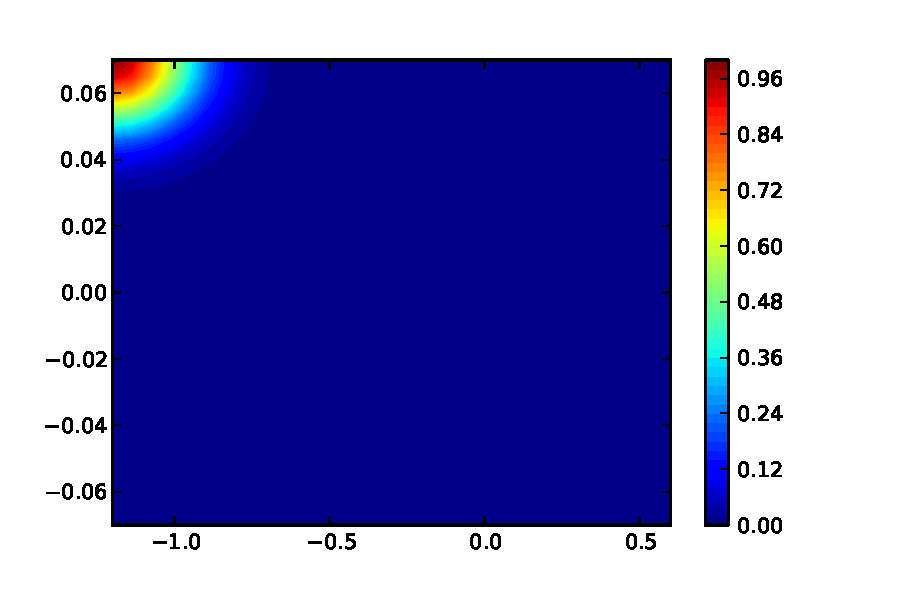
\includegraphics[width=.13\textwidth]{Figures/Mountain_car_psi_6x0}};
\node at (0,-1) {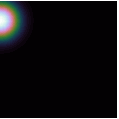
\includegraphics[width=.13\textwidth]{Figures/Mountain_car_psi_5x0}};
\node at (0,-2) {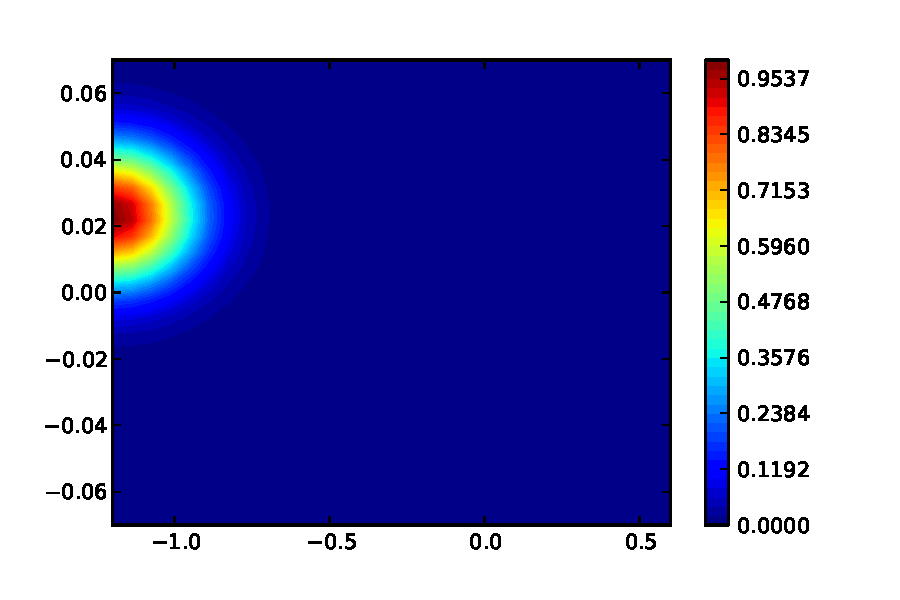
\includegraphics[width=.13\textwidth]{Figures/Mountain_car_psi_4x0}};
\node at (0,-3) {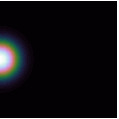
\includegraphics[width=.13\textwidth]{Figures/Mountain_car_psi_3x0}};
\node at (0,-4) {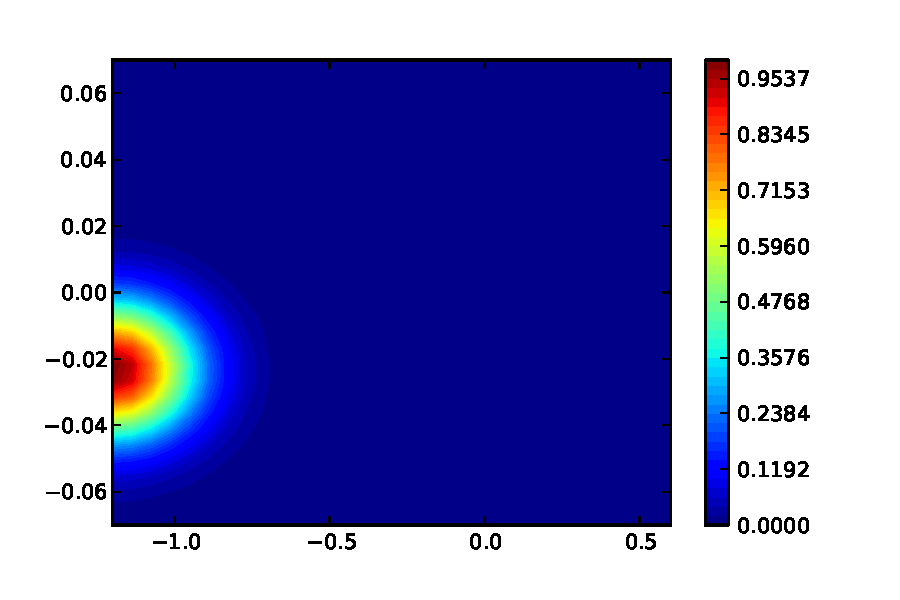
\includegraphics[width=.13\textwidth]{Figures/Mountain_car_psi_2x0}};
\node at (0,-5) {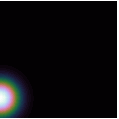
\includegraphics[width=.13\textwidth]{Figures/Mountain_car_psi_1x0}};
\node at (0,-6) {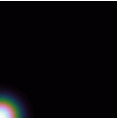
\includegraphics[width=.13\textwidth]{Figures/Mountain_car_psi_0x0}};
                                          
\node at (1,-0) {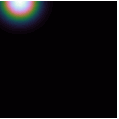
\includegraphics[width=.13\textwidth]{Figures/Mountain_car_psi_6x1}};
\node at (1,-1) {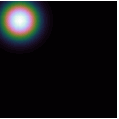
\includegraphics[width=.13\textwidth]{Figures/Mountain_car_psi_5x1}};
\node at (1,-2) {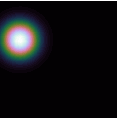
\includegraphics[width=.13\textwidth]{Figures/Mountain_car_psi_4x1}};
\node at (1,-3) {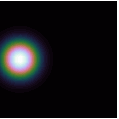
\includegraphics[width=.13\textwidth]{Figures/Mountain_car_psi_3x1}};
\node at (1,-4) {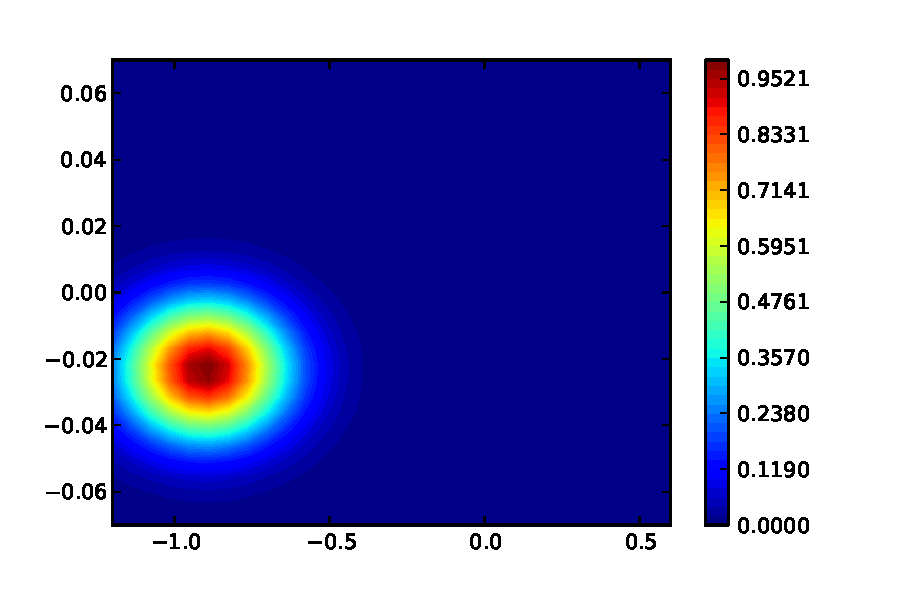
\includegraphics[width=.13\textwidth]{Figures/Mountain_car_psi_2x1}};
\node at (1,-5) {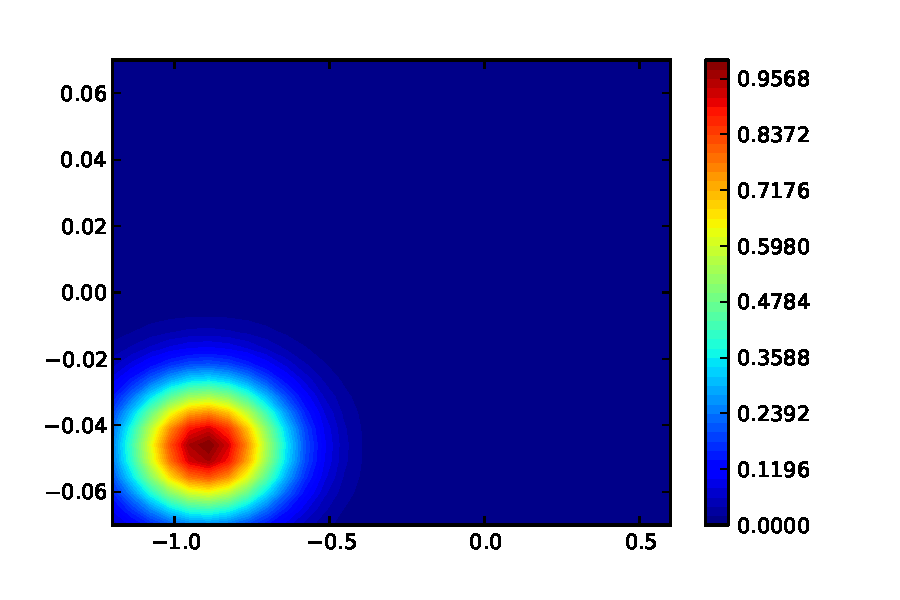
\includegraphics[width=.13\textwidth]{Figures/Mountain_car_psi_1x1}};
\node at (1,-6) {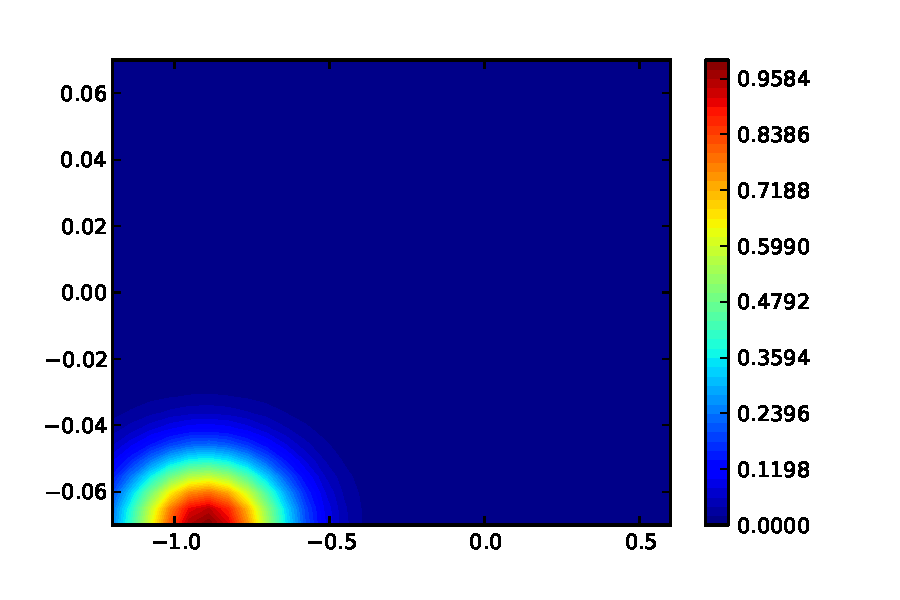
\includegraphics[width=.13\textwidth]{Figures/Mountain_car_psi_0x1}};
                                          
\node at (2,-0) {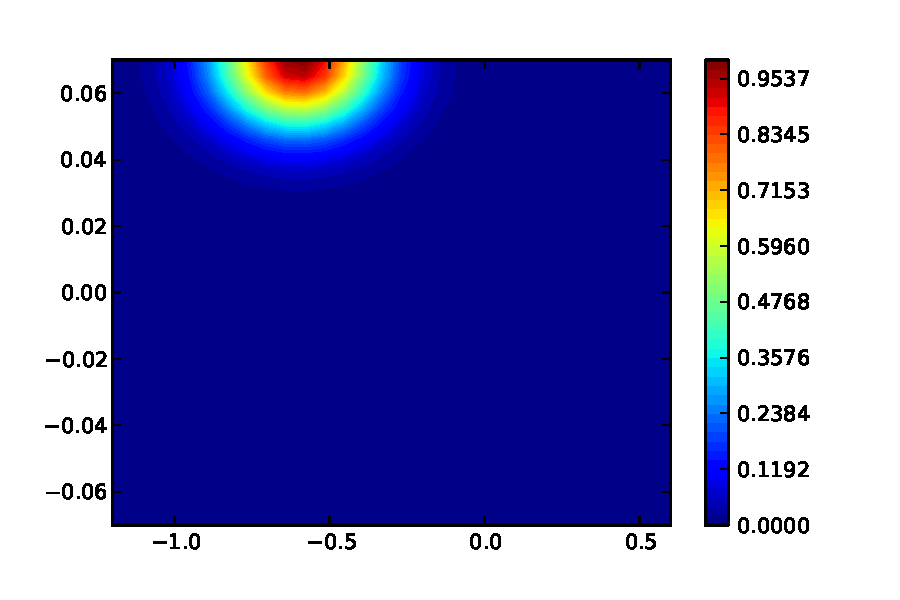
\includegraphics[width=.13\textwidth]{Figures/Mountain_car_psi_6x2}};
\node at (2,-1) {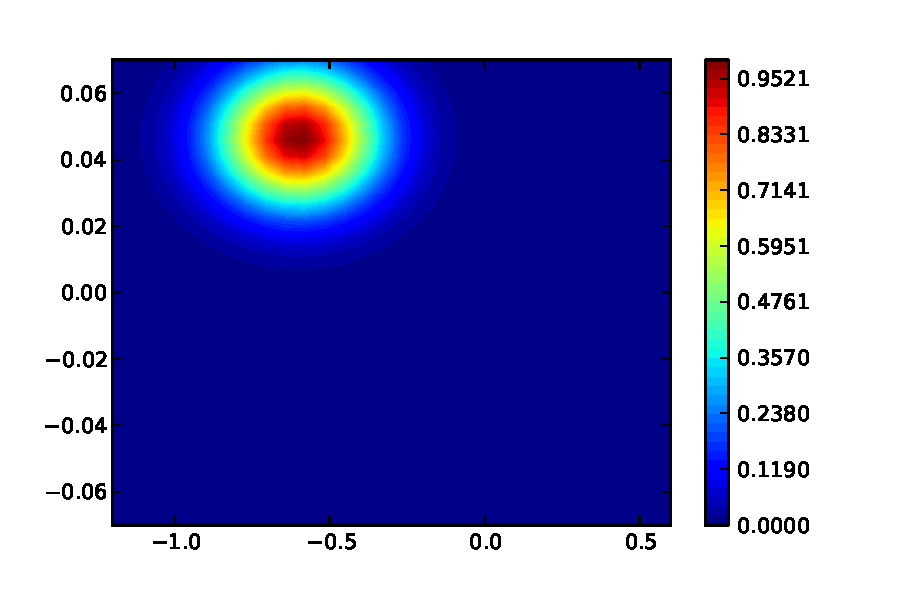
\includegraphics[width=.13\textwidth]{Figures/Mountain_car_psi_5x2}};
\node at (2,-2) {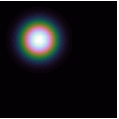
\includegraphics[width=.13\textwidth]{Figures/Mountain_car_psi_4x2}};
\node at (2,-3) {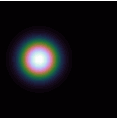
\includegraphics[width=.13\textwidth]{Figures/Mountain_car_psi_3x2}};
\node at (2,-4) {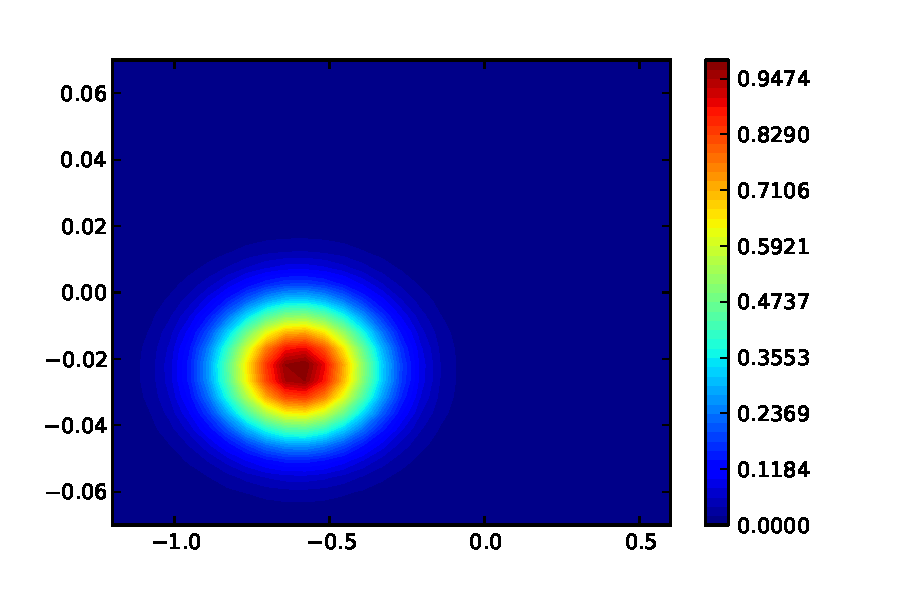
\includegraphics[width=.13\textwidth]{Figures/Mountain_car_psi_2x2}};
\node at (2,-5) {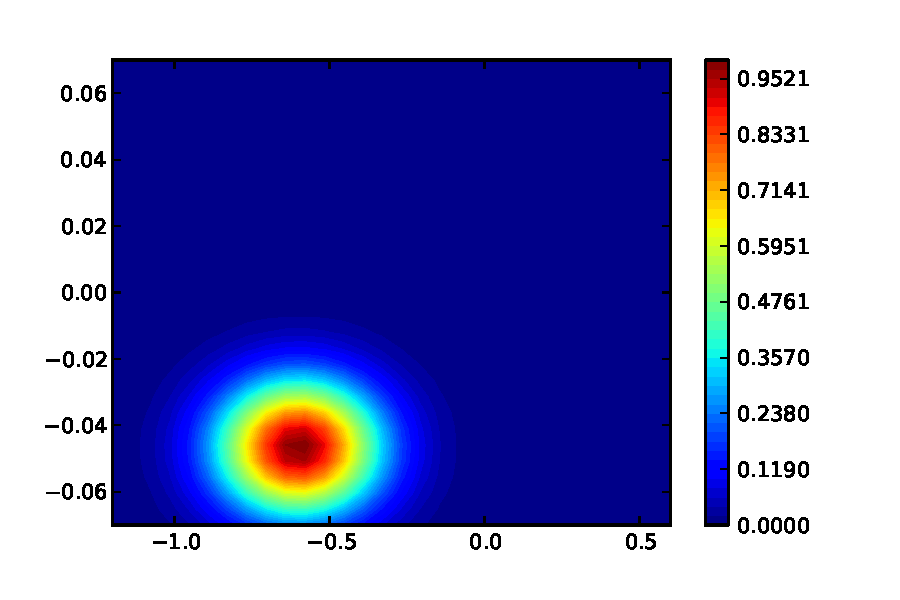
\includegraphics[width=.13\textwidth]{Figures/Mountain_car_psi_1x2}};
\node at (2,-6) {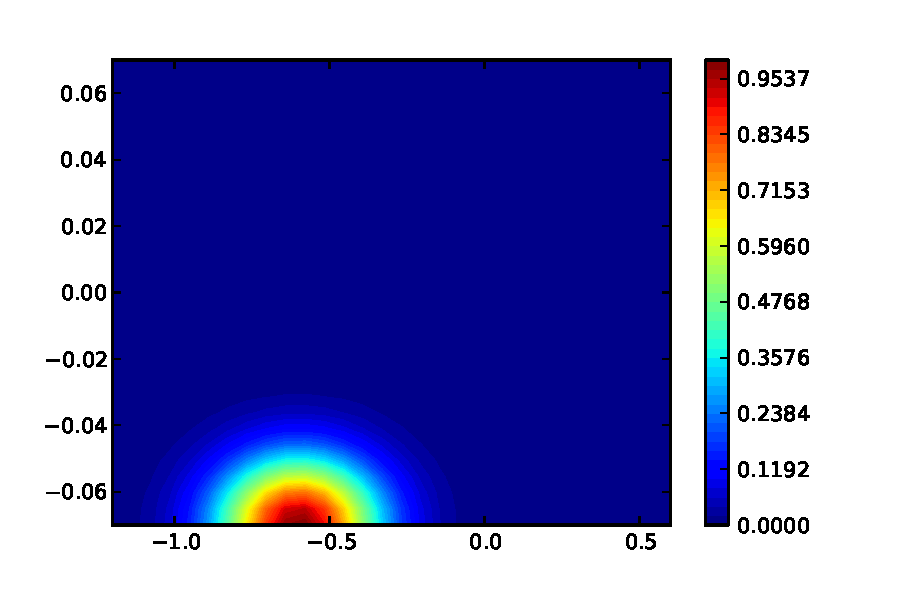
\includegraphics[width=.13\textwidth]{Figures/Mountain_car_psi_0x2}};
                                          
\node at (3,-0) {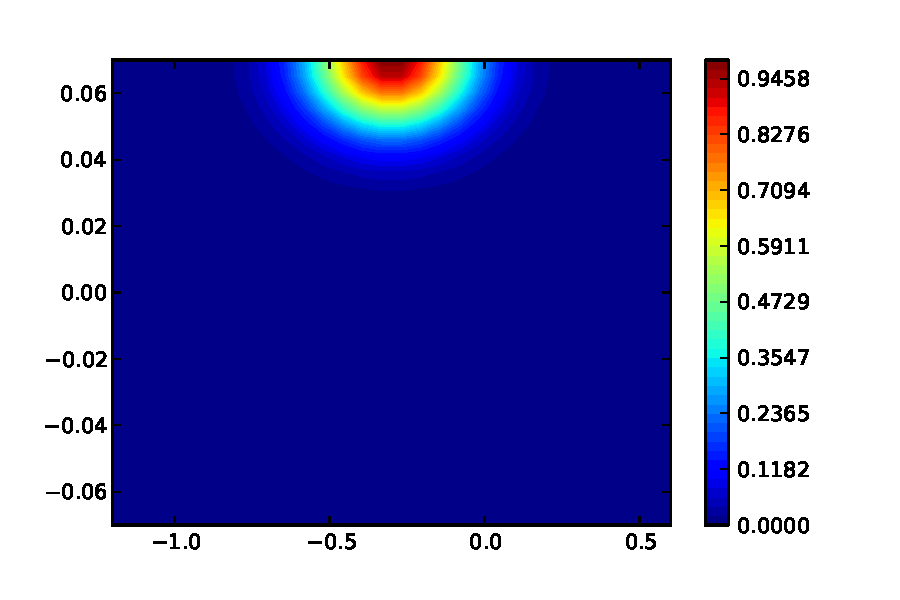
\includegraphics[width=.13\textwidth]{Figures/Mountain_car_psi_6x3}};
\node at (3,-1) {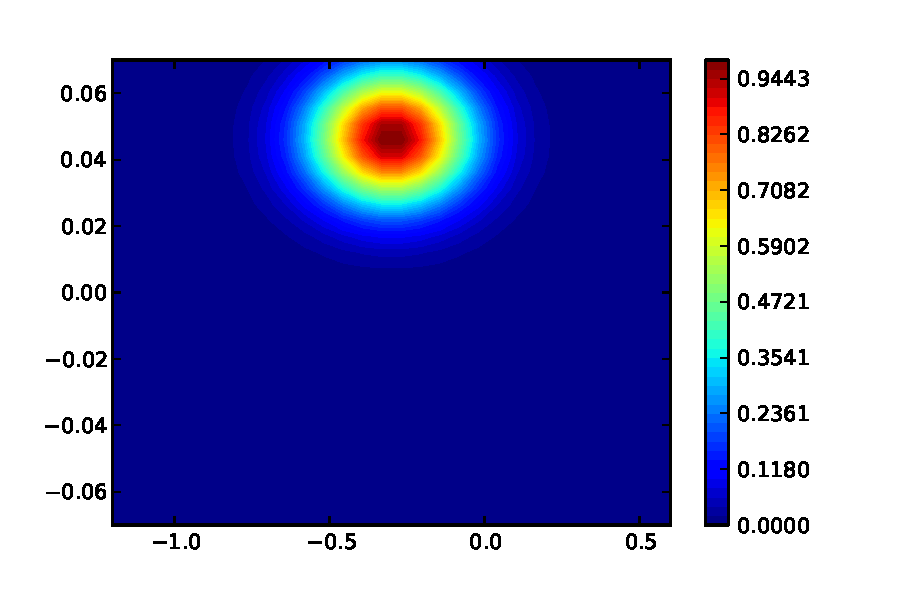
\includegraphics[width=.13\textwidth]{Figures/Mountain_car_psi_5x3}};
\node at (3,-2) {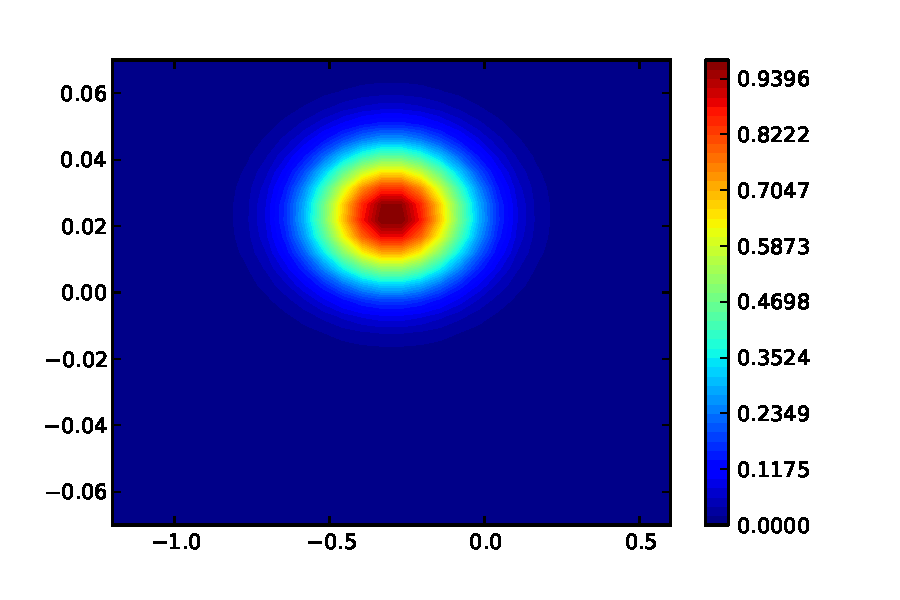
\includegraphics[width=.13\textwidth]{Figures/Mountain_car_psi_4x3}};
\node at (3,-3) {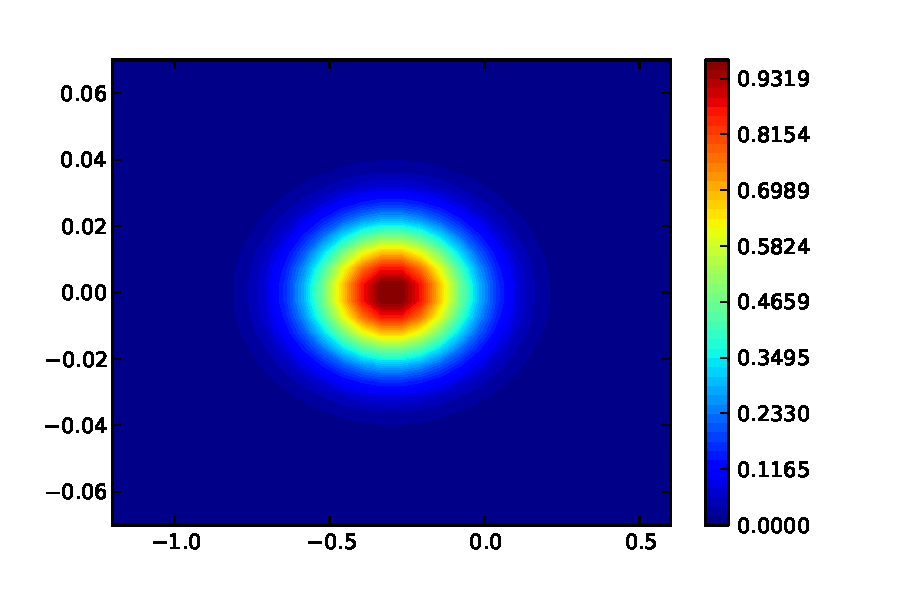
\includegraphics[width=.13\textwidth]{Figures/Mountain_car_psi_3x3}};
\node at (3,-4) {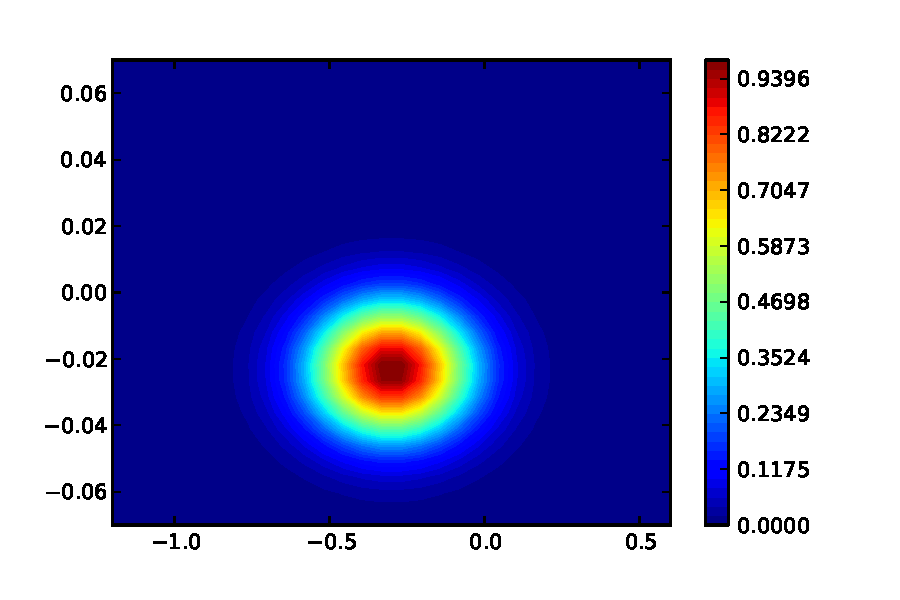
\includegraphics[width=.13\textwidth]{Figures/Mountain_car_psi_2x3}};
\node at (3,-5) {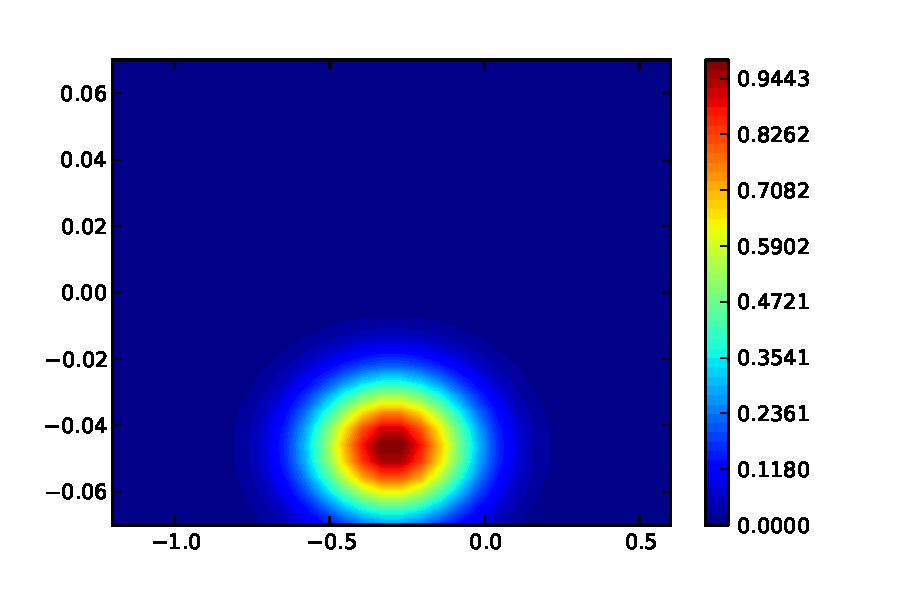
\includegraphics[width=.13\textwidth]{Figures/Mountain_car_psi_1x3}};
\node at (3,-6) {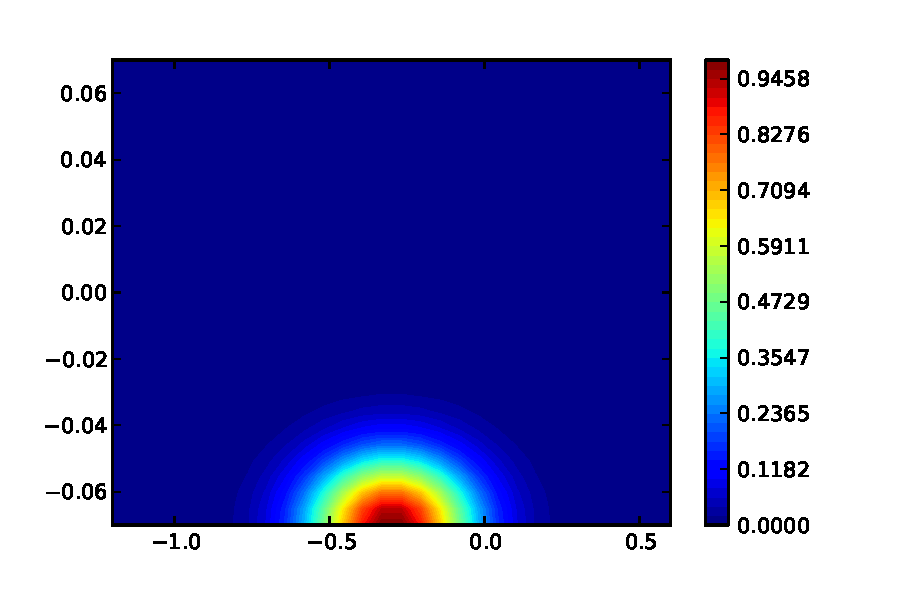
\includegraphics[width=.13\textwidth]{Figures/Mountain_car_psi_0x3}};
                                          
\node at (4,-0) {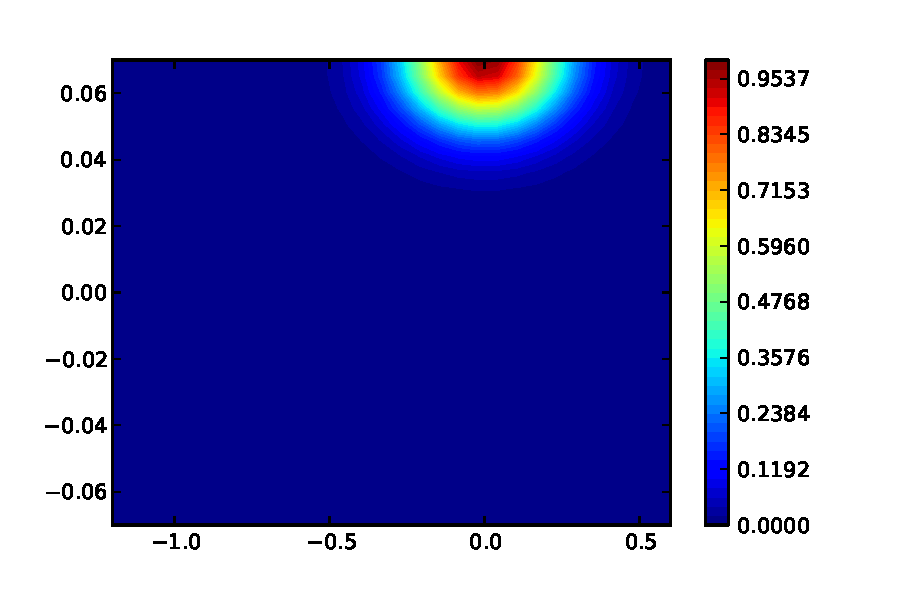
\includegraphics[width=.13\textwidth]{Figures/Mountain_car_psi_6x4}};
\node at (4,-1) {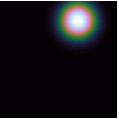
\includegraphics[width=.13\textwidth]{Figures/Mountain_car_psi_5x4}};
\node at (4,-2) {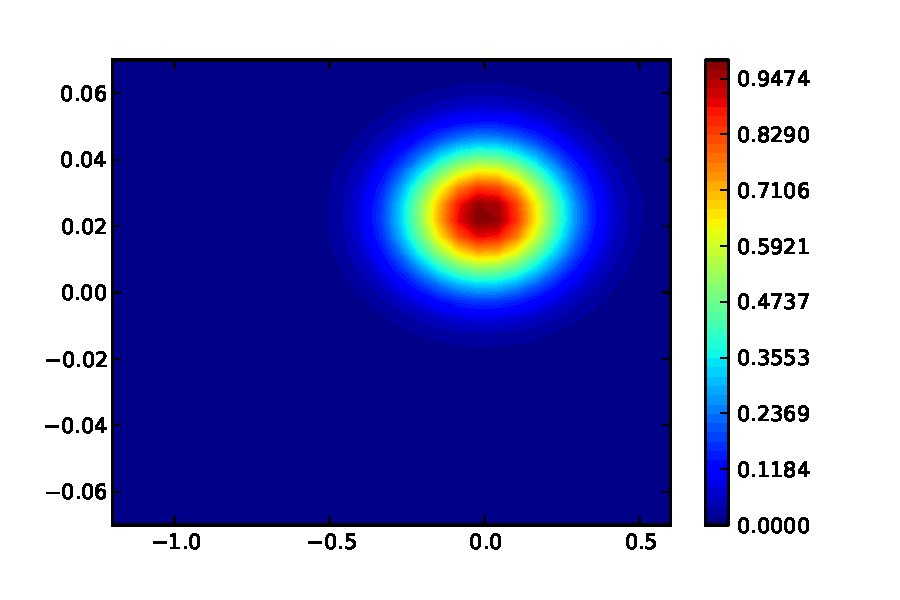
\includegraphics[width=.13\textwidth]{Figures/Mountain_car_psi_4x4}};
\node at (4,-3) {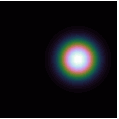
\includegraphics[width=.13\textwidth]{Figures/Mountain_car_psi_3x4}};
\node at (4,-4) {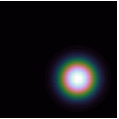
\includegraphics[width=.13\textwidth]{Figures/Mountain_car_psi_2x4}};
\node at (4,-5) {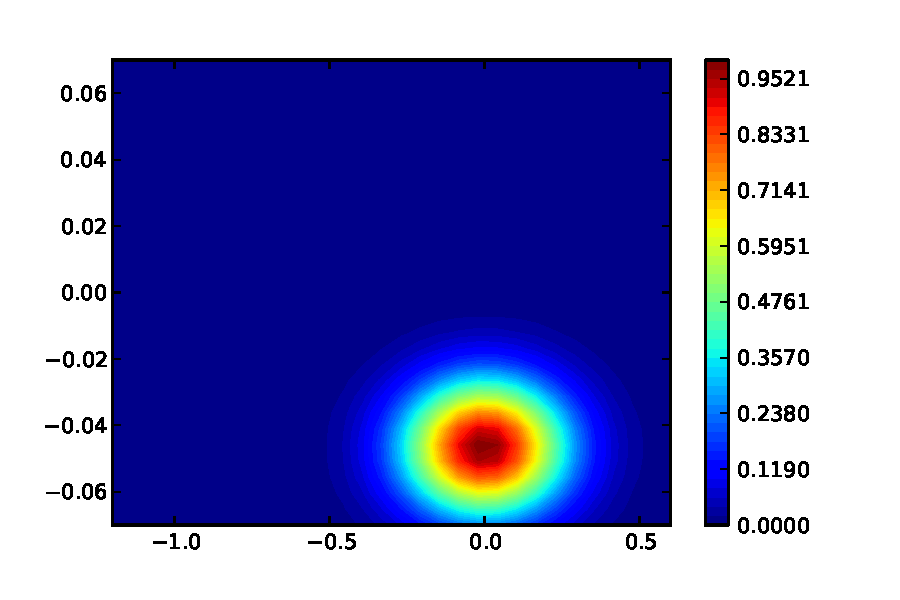
\includegraphics[width=.13\textwidth]{Figures/Mountain_car_psi_1x4}};
\node at (4,-6) {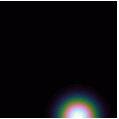
\includegraphics[width=.13\textwidth]{Figures/Mountain_car_psi_0x4}};
                                          
\node at (5,-0) {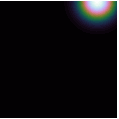
\includegraphics[width=.13\textwidth]{Figures/Mountain_car_psi_6x5}};
\node at (5,-1) {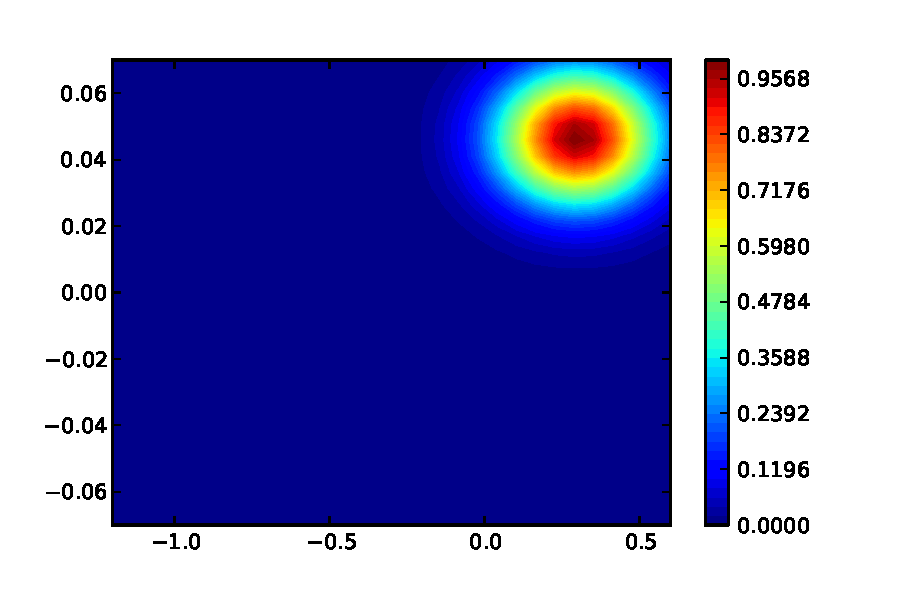
\includegraphics[width=.13\textwidth]{Figures/Mountain_car_psi_5x5}};
\node at (5,-2) {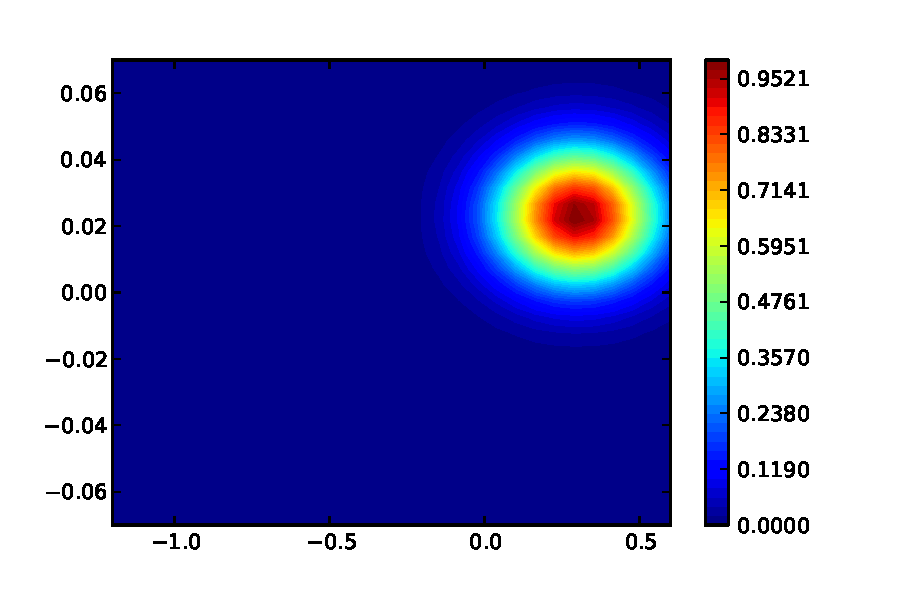
\includegraphics[width=.13\textwidth]{Figures/Mountain_car_psi_4x5}};
\node at (5,-3) {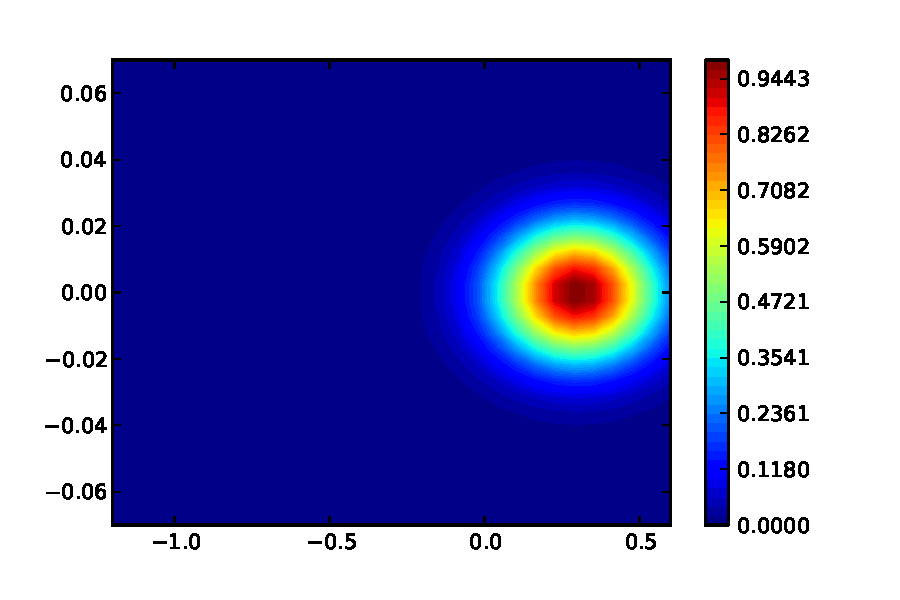
\includegraphics[width=.13\textwidth]{Figures/Mountain_car_psi_3x5}};
\node at (5,-4) {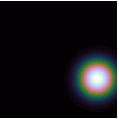
\includegraphics[width=.13\textwidth]{Figures/Mountain_car_psi_2x5}};
\node at (5,-5) {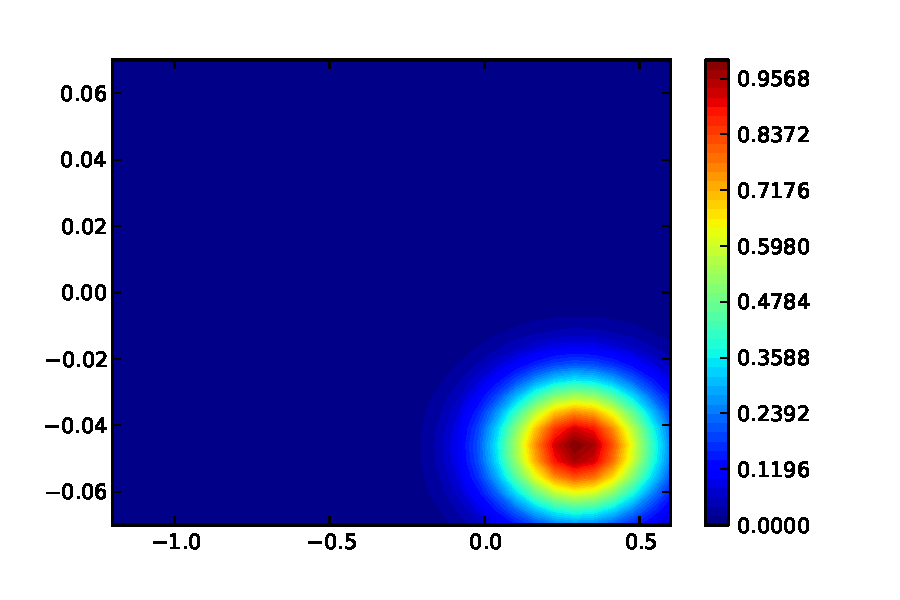
\includegraphics[width=.13\textwidth]{Figures/Mountain_car_psi_1x5}};
\node at (5,-6) {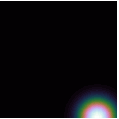
\includegraphics[width=.13\textwidth]{Figures/Mountain_car_psi_0x5}};
                                          
\node at (6,-0) {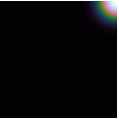
\includegraphics[width=.13\textwidth]{Figures/Mountain_car_psi_6x6}};
\node at (6,-1) {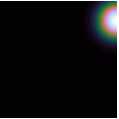
\includegraphics[width=.13\textwidth]{Figures/Mountain_car_psi_5x6}};
\node at (6,-2) {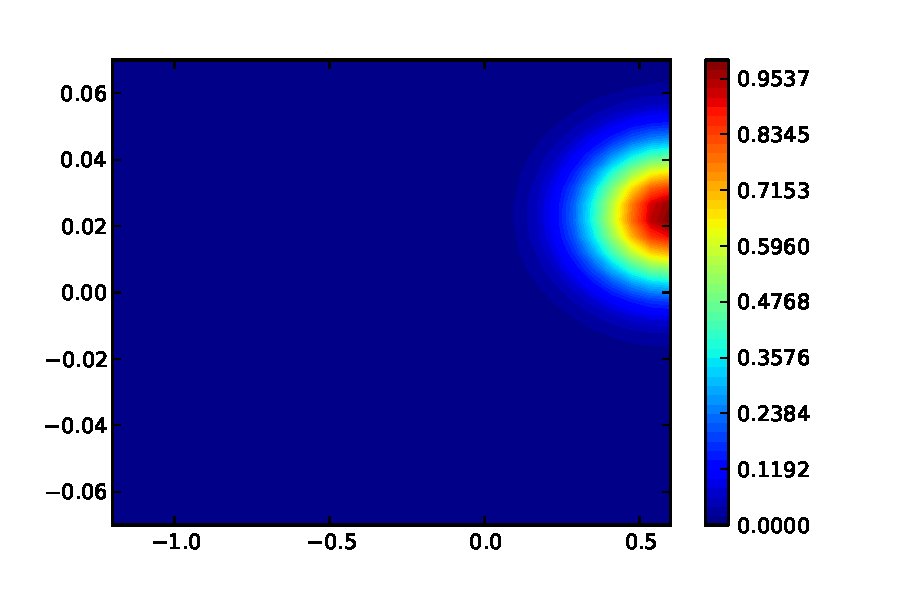
\includegraphics[width=.13\textwidth]{Figures/Mountain_car_psi_4x6}};
\node at (6,-3) {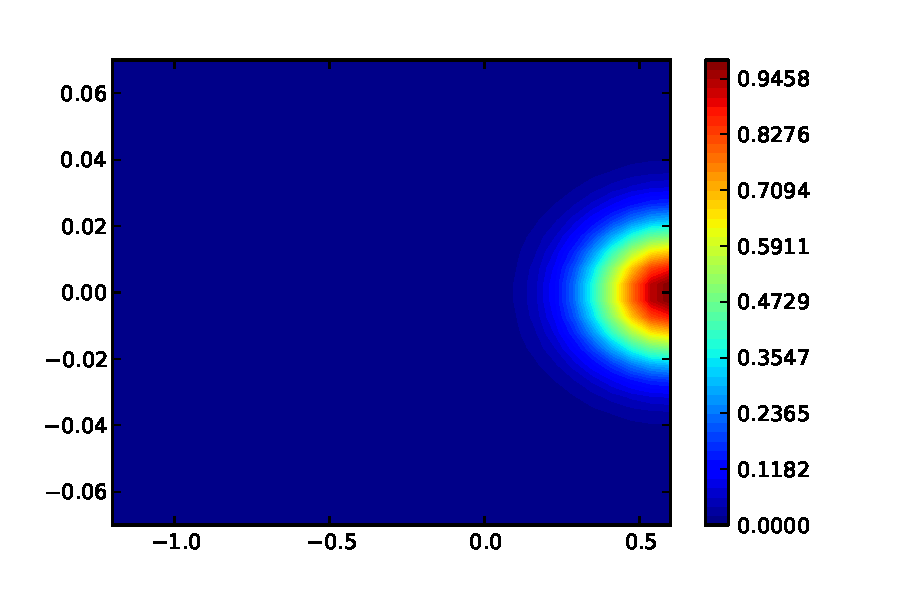
\includegraphics[width=.13\textwidth]{Figures/Mountain_car_psi_3x6}};
\node at (6,-4) {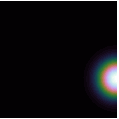
\includegraphics[width=.13\textwidth]{Figures/Mountain_car_psi_2x6}};
\node at (6,-5) {\includegraphics[width=.13\textwidth]{Figures/Mountain_car_psi_1x6}};
\node at (6,-6) {\includegraphics[width=.13\textwidth]{Figures/Mountain_car_psi_0x6}};
\end{tikzpicture}
\caption[Attributs gaussiens sur le problème du \glstext{mountaincar}]{Attributs gaussiens sur le problème du \gls{mountaincar}. L'espace d'état est pavé de $7\times 7 = 49$ gaussiennes elliptiques dont les centres sont répartis à équidistance. Les variances sont les mêmes pour toutes les gaussiennes et dépendent de la plage de valeurs sur une dimension. Toute fonction aux variations raisonnables peut être approximée de manière correcte par une somme pondérée de ces gaussiennes. Cette représentation est à comparer à la Figure 2.2 
% \autoref{fig:mountain_car_mu}
où est présenté l'attribut moyen qui, lui, prend en compte la dynamique temporelle du problème.}
\label{fig:mountain_car_psi}
\end{figure*}
\clearpage
\subsection{Classification à marge structurée}
\label{sec-2-1-4}
\label{hier-taskar}

Illustrons ce propos par l'étude d'une approche de classification qui utilise une fonction de score linéairement paramétrée sur l'espace d'attribut état-action $\featurestateactionspace$ \citep{taskar2005learning}.

Le principe quasi-ubiquitaire en classification\footnote{Les arbres de décision formant un contre-exemple notable \citep{safavian1991survey}.
 } de la fonction de score est le suivant : à chaque couple état-action une fonction $\classifscorefunc$ associe un score. Pour associer une action à un état, le classifieur passe simplement en revue toutes les actions (on voit donc l'intérêt d'un petit espace d'action) et choisit celle qui associée à cet état obtient le score le plus haut :
\begin{align}
\classifscorefunc &\in \twosetsfunctions{\statespace \times \actionspace}{\reals},\\
\forall \state, \classifpolicy(\state) &\in \arg\max_{\action \in \actionspace} \classifscorefunc(\state,\action).
\label{eq:classifscore}
\end{align}
Apprendre une bonne fonction de score permet donc de résoudre le problème de classification. L'approche proposée dans \citep{taskar2005learning} prend le parti d'une fonction de score linéaire :
\begin{equation}
q_{\paramclassif}(\state,\action) = \transpose{\paramclassif}\featurestateactionfunc_{\classifscorefunc}(\state,\action).
\end{equation}
Ce que nous cherchons maintenant est donc un bon vecteur de paramètres $\paramclassif$.


Considérant que nous disposons d'un vecteur d'attributs permettant de continuer, examinons à des fins d'illustration le problème que \citet{taskar2005learning} se proposent de résoudre, problème que nous retrouverons \autoref{hier-scirl}. Il s'agit d'un problème d'optimisation convexe sous contraintes\footnote{Pour voir que les variables $\slack_{\datasetindex}$ sont positives, on peut poser $a=a_i$ (et considérer que $\margin(s_i,a_i)=0$).
 } :
\begin{align}
&\min\limits_{\slack \in \reals_{+}} \frac{\lambda}{2}\|\omega\|^2+{1\over \nbsamples}\sum\limits_{\datasetindex=1}^{\nbsamples}\slack_{\datasetindex}\\
\textrm{sous les contraintes }\forall \datasetindex, \classifscorefunc_{\paramclassif}(\state_{\datasetindex},\action_{\datasetindex}) \geq &\max\limits_{\action \in \actionspace}(\classifscorefunc_{\paramclassif}(\state_{\datasetindex},\action) + \margin(\state_{\datasetindex},\action)) - \slack_{\datasetindex}.
\end{align}
La fonction objectif cherche naturellement à réduire les variables d'écart $\slack_{\datasetindex}$ tandis que les contraintes sont telles que la valeur prise par la fonction de score $\classifscorefunc_{\paramclassif}$ en un couple $(\state_{\datasetindex}, \action_{\datasetindex})$ correspondant à une décision experte est supérieure ou égale au meilleur score. Elle doit être non seulement supérieure au score seul, mais supérieure d'une certaine marge $\margin(\state_{\datasetindex},\action)$ qui contribue à donner à ce classifieur sa capacité de généralisation. En effet, on constate que si $\margin$ est uniformément nulle, alors parvenir à minimiser parfaitement la fonction de coût se réduit à apprendre par cœur la base d'exemples, c'est-à-dire à probablement subir les effets du sur-apprentissage. Fixer 
\begin{equation}
\margin(\state_{\datasetindex},\action) = \begin{cases}
0 &\textrm{si }\action = \action_{\datasetindex}\\
1 &\textrm{si }\action \neq \action_{\datasetindex}
\end{cases}
\label{eq:margin}
\end{equation}
permet de donner aux choix de l'expert un score strictement supérieur aux scores des autres choix. \citet{taskar2005learning} précisent qu'il est possible d'adapter la marge $\margin$ en fonction de la qualité des choix alternatifs, un bon choix correspondant à une petite marge. Nous verrons qu'en pratique la marge binaire que nous venons de suggérer fonctionne assez bien pour les problèmes qui nous intéressent.

La résolution informatique d'un problème d'optimisation convexe sous contraintes pouvant être malaisée, nous en cherchons une formulation plus simple (qui revient à celle employée dans \citep{ratliff2007imitation}) en constatant que si une contrainte de bon classement est violée, alors compte-tenu de la nature de la contribution empirique à la fonction objectif, la valeur de la variable d'écart correspondante est obtenue en traitant ladite contrainte comme une contrainte-égalité :
\begin{equation}
\slack_{\datasetindex} =  \max\limits_{\action \in \actionspace}(\classifscorefunc_{\paramclassif}(\state_{\datasetindex},\action) + \margin(\state_{\datasetindex},\action)) - \classifscorefunc_{\paramclassif}(\state_{\datasetindex},\action_{\datasetindex}).
\end{equation}
En posant :
\begin{align}
\best{\action}_{\datasetindex} &= \arg\max_{\action \in \actionspace}(\classifscorefunc_{\paramclassif}(\state_{\datasetindex},\action) + \margin(\state_{\datasetindex},\action))\\
 &= \arg\max_{\action \in \actionspace} (\transpose{\paramclassif}\featurestateactionfunc_{\classifscorefunc}(\state_{\datasetindex},\action) + \margin(\state_{\datasetindex},\action)),
 \end{align}
et en faisant monter les contraintes dans la fonction objectif, on obtient alors une simple fonction de coût à minimiser :
\begin{align}
\structuredcost(\paramclassif) &= {1\over \nbsamples} \sum_{\datasetindex=1}^{\nbsamples} (\classifscorefunc_{\paramclassif}(\state_{\datasetindex},\best{\action}_{\datasetindex}) + \margin(\state_{\datasetindex},\best{\action}_{\datasetindex}) - \classifscorefunc_{\paramclassif}(\state_{\datasetindex},\action_{\datasetindex})) +\frac{\lambda}{2}\|\omega\|^2\\  &= {1\over \nbsamples} \sum_{\datasetindex=1}^{\nbsamples} (\transpose{\paramclassif}\featurestateactionfunc_{\classifscorefunc}(\state_{\datasetindex},\best{\action}_{\datasetindex}) + \margin(\state_{\datasetindex},\best{\action}_{\datasetindex}) - \transpose{\paramclassif}\featurestateactionfunc_{\classifscorefunc}(\state_{\datasetindex},\action_{\datasetindex}))+\frac{\lambda}{2}\|\omega\|^2.
\end{align}
Cette fonction n'est pas différentiable à cause de l'opérateur non-linéaire $\max$ caché dans le terme $\best{\action}_{\datasetindex}$, mais la généralisation du gradient qu'est le sous-gradient permet de contourner cette difficulté.
Le sous-gradient de la fonction de coût est :
\begin{equation}
\subgrad\structuredcost(\paramclassif) = \sum_{\datasetindex=1}^{N}(\featurestateactionfunc_{\classifscorefunc}(\state_{\datasetindex},\best{\action}_{\datasetindex}) - \featurestateactionfunc_{\classifscorefunc}(\state_{\datasetindex},\action_{\datasetindex}))+\lambda \omega,
\end{equation}
il est donc possible de résoudre le problème d'optimisation original en effectuant une simple descente de sous-gradient pour minimiser la fonction de coût $J(\paramclassif)$, comme cela est décrit dans l'\autoref{alg:taskar}.
\begin{algorithm}
\Entree{
Une base d'entraînement établie par l'expert $\satrace{\expertpolicy}$\;}
\Donnees{
Une fonction d'attribut $\featurestateactionfunc_{\classifscorefunc}$\;
}
\Sortie{Une règle de décision $\classifpolicy$}
Initialiser $\paramclassif$ arbitrairement\;
Procéder à la descente de sous-gradient dont le sous-gradient est :
\begin{equation*}
\subgrad\structuredcost(\paramclassif) = \sum_{\datasetindex=1}^{N}\left[\featurestateactionfunc_{\classifscorefunc}\left(\state_{\datasetindex},\max_{\action\in\actionspace}\transpose{\paramclassif}\featurestateactionfunc(\state_{\datasetindex},\action) + \margin(\state_{\datasetindex},\action)\right) - \featurestateactionfunc_{\classifscorefunc}(\state_{\datasetindex},\action_{\datasetindex})\right] + \lambda \omega\;
\end{equation*}
\Retour{\begin{equation*}
\classifpolicy : \state \rightarrow \classifpolicy(\state) \in \arg\max_{\action\in\actionspace} \transpose{\paramclassif}\featurestateactionfunc_{\classifscorefunc}(\state,\action)
\end{equation*}}
\caption{Algorithme de classification structurée}
\label{alg:taskar}
\end{algorithm}


Nous avons présenté cette technique de classification plus en détail à des fins d'illustration de l'importance du choix des attributs, et également car nous la retrouverons \autoref{hier-scirlinstan} lorsque nous nous intéresserons à une nouvelle technique d'\gls{irl}.

Il existe bien d'autres moyens de faire de la classification, comme par exemple les \gls{svm}.
\subsection{\glsentrytext{svm}}
\label{sec-2-1-5}
\label{hier-svm}


    Une \gls{svm} est un séparateur linéaire. Plus précisément, une \gls{svm} va chercher, dans un espace de représentation des entrées, l'hyperplan de marge maximale séparant les données : d'un côté de l'hyperplan se trouvent toutes les entrées associées à une certaine étiquette, et de l'autre côté se trouvent les entrées associées à l'autre étiquette. Il faut positionner l'hyperplan dans l'espace de représentation de manière à maximiser la distance entre celui-ci et les données.

    Il est illusoire de croire que l'espace de description est construit d'une manière qui permette à un hyperplan de séparer les exemples sans erreur. Le classifieur à fonction de score paramétrée linéairement que nous avons décrit précédemment compense cela par une projection dans un espace d'attributs (ou espace de représentation) $\featurestateactionspace$. Les \gls{svm} utilisent une technique similaire, l'idée est de remplacer les produits scalaires $\scalarprod{\state}{\state'}_{\statespace}$ qui apparaitraient dans l'algorithme par un produit scalaire $\scalarprod{\featurestatefunc(\state)}{\featurestatefunc(\state')}_{\Psi}$ dans l'espace d'attributs $\Psi$, dans l'espoir que les données soient linéairement séparables dans cet espace. L'astuce, dite astuce du noyau \citep{aizerman1964theoretical,boser1992training} est d'observer que les données n'apparaissent dans l'algorithme que par le biais de leur produit scalaire ; plutôt que de définir explicitement cet attribut $\featurestatefunc$ et de calculer le produit scalaire associé, un noyau $\kernel$ est défini. Pour peu que $\kernel$ satisfasse certaines conditions\footnote{\`A savoir être continu, symétrique et semi-défini positif.
 }, alors il existe \citep{mercer1909functions,berlinet2004reproducing} une fonction $\featurestatefunc$ telle que \footnote{Le noyau $\kappa$ engendre un \emph{Reproducing Kernel Hilbert Space} (RKHS) \citep{berlinet2004reproducing}.
 }:
\begin{equation}
\kernel(\state,\state') = \scalarprod{\featurestatefunc(\state)}{\featurestatefunc(\state')}_{\Psi}.
\end{equation} 

Un noyau populaire, le noyau gaussien :
\begin{equation}
\kernel(\state,\state')=\exp\left(- \frac{\|\state - \state'\|^2}{2 \sigma^2}\right),
\end{equation}
permet de manipuler le produit scalaire $\scalarprod{\featurestatefunc(\state)}{\featurestatefunc(\state')}_\Psi$ où  l'espace d'attributs $\Psi$ engendré par $\featurestatefunc$ est de dimension infinie.

Le modèle que nous venons de décrire est celui de la \gls{svm} à marge dure \citep{boser1992training}. Comme dans le cas du classifieur à marge de la \autoref{hier-taskar}, il est possible d'introduire des variables d'écart. On passe alors au modèle de la \gls{svm} à marge douce \citep{cortes1995support}.

Pour l'imitation, la multiplicité des actions possibles appelle l'utilisation d'une \gls{svm} multi-classe (M-SVM). Un modèle unifiant les machines de ce type est proposé dans \citep{guermeur2012generic}. Pour simplifier l'exposé nous nous sommes cantonné au cas bi-classe. Le classifieur à marge de la sous-section précédente peut être instancié (si l'on choisit convenablement les valeurs des hyper-paramètres) comme un cas particulier d'une \gls{svm}, mais les deux modèles ne sont pas équivalents dans leur forme générique.


Les \gls{svm} sont très populaires et de nombreux logiciels les mettent en œuvre. Il est donc facile de les mettre en œuvre sur les problèmes jouet que nous allons traiter ; Ce sont des classifieurs pour lesquels la sélection de modèle est assez bien maîtrisée (\citet{bonidal2013analyse} a récemment présenté une thèse abordant ce sujet).
\subsection{Imitation par apprentissage supervisé de la politique}
\label{sec-2-1-6}
\label{hier-myopie}

Apprendre la politique de l'expert de manière supervisée à l'aide d'une base d'exemples peut s'avérer efficace, comme le démontrent plusieurs approches. Dans \citep{ratliff2007imitation}, les auteurs utilisent le classifieur à marge décrit plus haut
pour apprendre une politique experte pour un problème de locomotion quadrupède et sur un problème de manipulation d'objets. Le choix des attributs est automatisé grâce à une technique de \gls{boosting} similaire à \citep{friedman2001greedy,mason1999functional}.

Le boosting permet de déplacer de manière intelligente le problème du choix des attributs, sans le régler totalement. Il reste en effet à construire l'espace où choisir les nouveaux attributs. Un espace trop simple ne permettrait pas de minimiser efficacement la fonction de coût, tandis qu'un espace trop riche permettrait de l'annuler, mais sans doute au prix d'un sur-apprentissage aux conséquences fâcheuses. C'est donc cet espace qui doit être construit afin de donner au classifieur ses capacités de généralisation. \citet{ratliff2007imitation} proposent d'utiliser un réseau de neurones.

Plus brutale\footnote{Puisqu'elle repose sur l'utilisation d'une base d'exemple exhaustive.
 }, l'approche de \citet{lecun2006off} utilise un \gls{cnn} (réseau de convolution) à 6 couches pour apprendre une association directe entre une image (stéréo) et un angle de braquage (la tâche à apprendre est la conduite d'un véhicule en terrain libre). Le problème de la généralisation est résolu en exigeant une base d'entraînement couvrant au maximum l'espace d'état. Les auteurs ne cachent pas la difficulté de constituer une telle base qui doit réunir des conditions de terrain et d'illumination variées tout en exigeant un comportement extrêmement cohérent et prédictible de la part de l'opérateur humain et ce sur un grand nombre de trajectoires (il faut réunir près d'une centaine de milliers d'échantillons). En contrepartie de ces efforts, la technique proposée est robuste et ne nécessite aucun travail d'ingénierie au niveau des attributs, puisque la politique apprise associe directement la sortie du capteur à la consigne de l'actuateur du robot. Bien que cela soit moins problématique aujourd'hui avec l'augmentation de puissance des équipements embarqués, elle semble également plus rapide (dans l'exploitation, non dans l'apprentissage) que l'état de l'art de l'époque. Elle améliore les résultats notamment par rapport à \gls{alvinn} \citep{pomerleau1993knowledge} en ceci que la résolution des caméras peut être augmentée sans une trop grande explosion du nombre de connexions du réseau grâce à l'usage de la convolution et non d'un réseau complètement connecté, et que la tâche apprise est plus difficile, il s'agit de conduire en terrain libre et non de suivre une route.

Nous venons de voir deux outils différents (\gls{boosting} et réseau de convolution) permettant d'apprendre une politique sans contrôler le système, de manière supervisée, avec une intervention humaine minimale : soit l'on dispose de suffisamment de données pour que le risque empirique soit proche du risque réel, soit l'on construit des attributs tels que l'apprentissage au mieux (en minimisant une fonction de coût exprimée sur les données) ne soit pas un apprentissage par cœur, mais un apprentissage généralisant sur tout l'espace d'état. Apprendre une politique de manière locale, c'est-à-dire en se concentrant trop sur une base de données ne couvrant pas tout l'espace d'état, n'est pas satisfaisant. Cela donne un résultat fragile, l'agent sera en effet pris au dépourvu s'il a à contrôler le système dans une configuration différente de celles sur lesquelles il a été entraîné : il ne dispose ni d'information relative au comportement de l'expert dans une telle situation, ni d'information sur la tâche à accomplir qui lui permettraient de déduire ce que pourrait être ce comportement.

L'idée de demander ces échantillons de manière interactive a été proposée afin de minimiser la quantité de données nécessaire à l'apprentissage de la politique experte. Un exemple d'une telle approche est décrit par \citet{chernova2007confidence}. Des \gls{gmm} sont appris à partir d'une base de données experte de départ, puis l'agent applique la politique apprise tout en demandant à l'expert, lorsque l'incertitude est trop grande, de lui fournir un échantillon supplémentaire. Cette approche permet de limiter la redondance de la base d'entraînement et de guider l'échantillonnage vers les zones intéressantes de l'espace d'état, ce qui est également une solution au problème de la généralisation : quand l'agent ne sait pas généraliser, il demande à l'expert. Cela est connu sous le nom d'apprentissage actif \citep{cohn1996active}.

Une autre approche d'apprentissage actif est l'algorithme \gls{smile} proposé par \citet{ross2010efficient}. A chaque itération $\timeindex$ une politique mixante $\policy_{\timeindex}$ \footnote{Une politique mixante est une sorte de méta-politique qui choisit aléatoirement quelle politique exécuter parmi un ensemble de politiques, généralement de manière non uniforme, certaines politiques étant préférées à d'autres.
 } est définie à l'aide d'une politique de classification $\classifpolicy$ apprise sur une base de données experte. Cette base de données est construite sur la distribution d'états induite par l'application de la politique mixante de l'itération précédente, $\policy_{\timeindex-1}$. La politique mixante à l'itération $\timeindex$ est une pondération de trois politiques : la politique mixante de l'itération précédente $\policy_{\timeindex-1}$, la politique apprise par le classifieur à l'itération courante $\classifpolicy$ et la politique initiale $\policy_{0}$ qui se réfère systématiquement à l'expert. L'algorithme \gls{dagger} (\citet{ross2010reduction}) maintient une base d'entraînement de plus en plus grande grâce à une politique mixante entre une politique de classification et la politique de l'expert. Les états-actions traversés par la politique mixante courante ayant donné lieu à une décision de l'expert sont ajoutés à la base d'entraînement et à l'itération suivante le classifieur est entraîné sur la nouvelle base. Le poids accordé à la politique de l'expert diminue pour laisser petit à petit le contrôle à l'agent. La logique derrière ces deux approches est d'éviter de faire de l'apprentissage supervisé sur la distribution fixe de l'expert $\expertdistrib$, pour la remplacer par la distribution que l'agent rencontrera vraiment, et qui tient compte des erreurs qu'il peut parfois commettre. Grâce au schéma interactif où l'expert donne peu à peu le contrôle à l'agent, l'expert est parfois entraîné loin de sa distribution et peut alors montrer à l'agent comment corriger l'erreur que celui-ci a commise.

L'apprentissage direct de la politique experte est parfois intégré à un cadre plus large, où les notions de hiérarchie et de but apparaissent.

La classification par arbre de décision a été appliquée à l'apprentissage d'un plan de vol par \citet{sammut1992learning}. L'application est ambitieuse ; \emph{apprendre} \footnote{La conception par des humains d'un système de pilotage automatique précède l'ordinateur puisque la démonstration d'un prototype a été faite à Paris en 1914.
 } à piloter un avion, même en simulation, n'est pas une mince affaire puisqu'il faut en temps réel prendre en compte un grand nombre de facteurs pour décider d'une action parmi un éventail assez large. L'apprentissage automatique nécessite un grand nombre d'échantillons. Un comportement cohérent est exigé de l'expert humain (à un point tel que les démonstrations de deux experts ne peuvent être mélangées en une seule base d'entraînement). L'aspect automatique de l'approche est limité à l'apprentissage d'une politique par phase de vol. La détection de la phase de vol courante et donc le choix de la politique de contrôle à appliquer est effectué par des règles d'origine humaine.

De fait, cette approche a été le point de départ de nombreuses améliorations. Le travail présenté par \citet{stirling1995churps} (appelé \gls{churps}) consiste à déduire un contrôleur à partir d'une description du modèle d'évolution du système et du but à atteindre. Pour automatiser la création de ces descriptions, tâche réclamant un travail difficile car nécessitant de décrire des mécanismes précis à l'aide d'un langage contraignant, \citet{bain2000framework} proposent d'utiliser les données de l'expert. Les règles complexes ainsi apprises étant ajoutées à l'espace d'action, il est possible d'apprendre de manière automatique un classifieur plus concis que celui de \citet{sammut1992learning}, et nécessitant moins de données expertes. L'architecture proposée utilise la logique du premier ordre et donc le raisonnement symbolique. Cela permet d'introduire explicitement des connaissances expertes dans le système. Ces connaissances peuvent être acquises semi-automatiquement : les prédicats sont construits à la main et les paramètres sont appris grâce aux données de vol comme le proposent \citet{srinivasan1998inductive}. La sémantique des symboles (ici, virage, altitude, trajectoire de vol, etc.) est très liée au problème concerné. Retrouver la puissance des techniques d'apprentissage symbolique sur un autre problème nécessite d'effectuer de nouveau le difficile travail de définition des symboles et prédicats. D'autres éléments potentiellement rédhibitoires sont la mauvaise gestion des fluctuations aléatoires dues à la dynamique et la difficulté d'exprimer la tâche à accomplir en utilisant un langage symbolique. Dans une approche hybride symbolique/numérique, \citet{shiraz1997combining} proposent à l'expert soit de décrire la tâche symboliquement, soit d'en démontrer l'exécution. Les phases les plus délicates (par exemple l'atterrissage) n'ont pu être décrites et ont été démontrées. La facilité d'exploitation des règles symboliques rentre en conflit avec la difficulté qu'il y a à les définir, à l'inverse la relative facilité de génération d'une base d'exemples se heurte à la difficulté qu'il y a à généraliser à partir de celle-ci.

Une autre approche utilise les notions de hiérarchie et de but, mais de manière quelque peu différente. Plutôt que d'utiliser la logique des prédicats, ce sont les principes de programmation impérative qui se voient assistés par l'apprentissage supervisé. Dans \citep{saunders2006teaching}, ce sont les \gls{knn} qui sont utilisés pour l'apprentissage supervisé d'une politique. Les attributs sont construits à la main à partir des valeurs de sortie des capteurs du robot, et portent une sémantique forte et explicite (distance, angle), donc pratique pour l'exploitation par un opérateur humain. Les problèmes de généralisation de l'apprentissage supervisé sont contournés par l'intégration dans un cadre beaucoup plus riche : l'opérateur humain peut élargir l'espace d'action à volonté, soit en définissant une séquence d'actions qui seront exécutées en série de manière déterministe, soit en proposant des exemples du comportement souhaité en précisant ou non un état-but correspondant à la situation dans laquelle on souhaite voir le robot une fois la politique exécutée. Ces exemples servent alors à l'apprentissage d'une politique de manière supervisée, cette politique est ajoutée en tant qu'action et son exécution pourra être déclenchée dans le cadre d'une autre politique, de niveau d'abstraction plus grand. Cette hiérarchisation des comportements permet de limiter l'effort humain, d'optimiser l'utilisation des exemples et de rapidement mettre en place des comportements complexes par la création de nouveaux niveaux d'abstraction. 

L'apprentissage supervisé est dans les approches que nous venons de citer utilisé comme sous routine d'un système beaucoup plus large, dans lequel l'expertise humaine explicite reste le moyen central permettant la généralisation des comportements.

Le principal problème de l'apprentissage direct de la politique de manière supervisé est, pour reprendre le terme de \citep{ratliff2009learning}, sa \emph{myopie}. Pour compenser le fait que l'on travaille au niveau d'abstraction le plus bas, celui du choix immédiat d'une action en fonction des informations contenues dans un état transitoire, les approches que nous venons de détailler font apparaître en filigrane la notion de but : l'expert n'agit en effet pas à tâtons mais dirige le système en fonction de critères qu'il paraît difficile d'exprimer au niveau d'une simple politique. On se repose donc sur une formulation plus ou moins explicite (dans le choix des attributs, dans la définition de la base d'exemples, dans l'introduction de règles logiques ou dans la définition d'une hiérarchie) de ce but, mais toujours d'origine humaine. Nous allons voir qu'il est possible de formaliser cette notion de but tout en continuant à travailler avec une politique et des échantillons semblables à ceux auxquels nous sommes habitués. Nous verrons par la suite que le but de l'expert, formalisé de cette manière, peut alors être automatiquement déduit d'une base d'échantillons acquise une fois pour toutes. 
\section{Cadre des \glsentrytext{mdp} pour la prise de décisions séquentielles}
\label{sec-2-2}
\label{hier-cadre}

Pour comprendre ce but de l'expert qu'il nous importe de connaître, ce n'est pas au niveau du choix état-action que décrit la politique qu'il faut regarder, mais à un niveau d'abstraction plus élevé : la dynamique que la politique de l'expert impose au système. La notion qui nous manque pour entamer le raisonnement est celle de l'effet d'une action. Nous ne nous sommes préoccupés que du choix de l'action en fonction de l'état courant sans nous soucier de ce que ce choix allait imposer comme contraintes sur le prochain état que l'agent va rencontrer. Afin de pouvoir considérer la politique de l'expert non plus comme un ensemble décousu d'associations état-action, mais comme un outil capable de produire des séquences d'actions pertinentes au sens d'un critère long terme, nous formalisons la notion de dynamique temporelle.
\subsection{Dynamique temporelle}
\label{sec-2-2-1}
\label{hier-tempdyn}


L'agent (qu'il s'agisse de l'expert ou d'un agent artificiel que l'on entraîne) aux manettes du système contrôle celui-ci non pas ponctuellement de temps à autres mais de manière cohérente sur un laps de temps durant lequel il devra opérer des actions de contrôle les unes après les autres. Il est donc naturel d'indexer ces actions et les états traversés par un indice temporel $\timeindex \in \llbracket 0;\infty\rrbracket$. Par exemple, cette formulation n'impose pas de pas d'échantillonnage constant, il s'agit ici d'ordonner les états et actions par ordre de causalité, ce qui incidemment correspond\footnote{\`A moins que \emph{Doctor Who} et \emph{Retour vers le futur} ne soient des documentaires.
 } à un indice temporel croissant, non pas de transcrire avec quelque fidélité les problèmes de l'échantillonnage temporel. Qui plus est cette formulation correspond à la réalité du contrôle numérique, intrinsèquement discret.

Pour prendre en compte les imperfections de la modélisation ou plus simplement parfois la nature réellement stochastique du problème, les effets d'une action qui sont décrits par une loi de probabilité, qui, informée d'un état $\state_{\timeindex}$ et d'une action $\action_{\timeindex}$, prédit vers quel état $\state_{\timeindex+1}$ le système va transiter. On note cela (encore une fois en identifiant loi de probabilité et densité de probabilité)\footnote{Avec $f\in\twosetsfunctions{A}{B\times C\times D}$, la notation $f(b,\cdot,d)$ désigne la fonction de $C$ dans $A$ : $c \rightarrow f(b,c,d)$.
 } :
\begin{equation}
\state_{\timeindex+1}\sim \transprobfunceval{\state_{\timeindex}}{\action_{\timeindex}}{\cdot}, \transprobfunc \in \twosetsfunctions{\statespace \times \actionspace \times \statespace}{[0;1]}.
\end{equation}
On constate que l'information sur l'état vers lequel on transite ne dépend que de l'état courant et de l'action courante, et non de la trajectoire. C'est la propriété de Markov qui donne son nom au \gls{mdp}.
La répétition du cycle consistant à choisir une action puis à transiter vers un nouvel état où l'agent choisit une action qui le fera transiter vers un nouvel état (etc.) forme une trajectoire. Les probabilités de transitions contraintes par une politique $\policy$ peuvent être dans le cas fini $\card{\statespace}<\infty$ représentées\footnote{En utilisant l'isomorphisme naturel entre $\statespace$ et $\llbracket 1,|\statespace|\rrbracket$.
 } par une matrice stochastique de taille $\card{\statespace}\times\card{\statespace}$ :
\begin{equation}
\transprobmat{\policy} = \matrixbyterm{\transprobfunceval{\state}{\policy(\state)}{\state'}}{\state}{\state'},
\end{equation}
où l'on note: $\left(f(i,j)\right)_{i,j}$ la matrice dont le terme à la ligne $i$ et à la colonne $j$ est $f(i,j)$.
Un agent de politique $\policy$ va visiter certains états plus que d'autres. Pour quantifier cela, il est possible d'utiliser la matrice des probabilités de transition que nous venons juste de définir. Le terme à la ligne $\state$ et à la colonne $\state'$ est la probabilité $\transprobfunceval{\state}{\policy(\state)}{\state'}$ que l'agent se trouve dans l'état $\state'$ au temps $\timeindex+1$ s'il était en $\state$ au temps $\timeindex$. Si l'on multiplie la matrice $\transprobmat{\policy}$ par elle même, le terme général (ligne $\state$, colonne $\state''$) du résultat est :
\begin{equation}
\sum_{\state'\in\statespace} \transprobfunceval{\state}{\policy(\state)}{\state'} \transprobfunceval{\state'}{\policy(\state')}{\state''},
\end{equation}
il s'agit de la probabilité pour l'agent de passer de $\state$ à $\state''$ en deux pas de temps. Si (et seulement si) l'agent peut espérer se trouver en chacun des états en temps fini, alors ce que l'on appelle la distribution stationnaire $\stationarydistrib{\policy}$ existe et est unique \citep{norris1998markov}. Elle est définie telle que :
\begin{equation}
\transpose{\stationarydistrib{\policy}} \transprobmat{\policy} = \transpose{\stationarydistrib{\policy}}.
\end{equation}
On peut donc la voir comme la probabilité pour l'agent de se trouver en un certain état, après un temps infini, quel que soit l'état de départ. Cette condition d'ergodicité que nous plaçons généralement sur le \gls{mdp} contraint par la politique de l'expert implique l'existence de la distribution stationnaire de l'expert $\expertdistrib$. Un \gls{mdp} contraint par une politique correspond à une chaine de Markov.
\subsection{Récompense et valeur}
\label{sec-2-2-2}

Dans les approches vues précédemment, le but était défini comme des valeurs spécifiques que doivent prendre certaines composantes de l'état (par exemple pour le pilotage, une certaine altitude) ou certaines valeurs de commandes acceptables dans certaines zones de l'espace d'état. Il est au premier abord assez naturel de définir une consigne comme cela. Pour peu que l'espace d'état-action soit construit d'une manière qui permet l'analyse sémantique, l'opérateur humain n'a pas trop de mal à exprimer ce qu'il souhaite que la machine fasse en définissant les états et actions désirables et ceux qu'il faut éviter. Charge à la machine de trouver comment se placer dans les états désirables en évitant les états problématiques. Nous formalisons cela sous la forme d'une fonction de récompense. Il s'agit d'un jugement local de l'intérêt qu'il y a à se trouver en un certain état ou appliquer certaines actions en certains états :
\begin{equation}
\rewardfunc \in \twosetsfunctions{\statespace\times \actionspace}{\reals}.
\end{equation}
Nous reviendrons \autoref{hier-recompense} sur la définition de la fonction de récompense.

Il faut maintenant que ce critère local donne lieu à un comportement globalement intéressant. Comment, à l'échelle d'une politique choisissant une action pour un état, parvenir à un contrôle tenant compte de la dynamique complète du système ? Il faut qu'une politique $\policy$ soit jugée dans son ensemble sur la trajectoire qu'elle impose à l'agent. Mathématiquement nous souhaitons optimiser la valeur de la politique\footnote{Pour simplifier, à l'avenir nous noterons le conditionnement par la dynamique induite par une politique comme cela : $\expectationknowing{\cdot}{s_0=s,\policy}$
 } :
\begin{align}
\label{eq:Vdefsum}
\rlvalue{\policy}{\rewardfunc}(\state,\action)&=\expectationknowing{\sum\limits_{\timeindex = 0}^{\infty} \discount^{\timeindex}\rewardfunc(\state_{\timeindex},\action_{\timeindex})}{\state_0 = s}\\
\textrm{avec }\forall \timeindex \in \llbracket 1;\infty\rrbracket, \state_{\timeindex} &\sim \transprobfunceval{\state_{\timeindex-1}}{\policy(\state_{\timeindex-1})}{\cdot}.
\end{align}
Comme l'horizon temporel est infini, pour s'assurer de la convergence de la somme, le facteur d'amortissement $\discount \in [0;1[$ est introduit. Une conséquence est la diminution d'attrait des récompenses loin dans le futur au profit de récompenses accessibles plus rapidement. Cela permet de récompenser l'agent qui effectue rapidement sa tâche.

La fonction de valeur, et un peu plus loin la fonction de qualité (\autoref{eq:qdef}) sont paramétrées par la fonction de récompense $\rewardfunc$ car par la suite nous serons amenés à étudier la valeur selon une certaine récompense d'une politique qui est optimale pour une autre récompense.

L'ensemble de l'espace d'état $\statespace$, de l'espace d'action $\actionspace$, des probabilités de transitions $\transprobfunc$, de la fonction de récompense $\rewardfunc$ et du facteur d'amortissement $\discount$ forment un \gls{mdp} $\mdpbis$ \citep{puterman1994markov}
\begin{equation}
\mdpbis = \left\{\statespace, \actionspace, \transprobfunc, \rewardfunc, \discount\right\}
\end{equation}
dans lequel le problème de la prise de décision séquentielle pour le contrôle optimal peut être formulé.

Nous recherchons une politique optimale $\optimalpolicy{\rewardfunc}$ telle qu'en tout état sa valeur soit supérieure ou égale à celle de tout autre politique $\pi$ :
\begin{equation}
\forall \state, \rlvalue{\optimalpolicy{\rewardfunc}}{\rewardfunc}(\state) \geq \rlvalue{\policy}{\rewardfunc}(\state).
\label{eq:optimalite}
\end{equation}
Pour résoudre ce problème, intéressons nous de plus près à l'expression de la valeur d'une politique, dont la définition, donnée \autoref{eq:Vdefsum}, peut être transformée en une expression récursive (grâce à la propriété de Markov) :
\begin{equation}
\label{eq:BellmanEval}
\rlvalue{\policy}{\rewardfunc}(\state) = \rewardfunc(\state,\policy(\state)) + \discount \sum_{\state'\in \statespace}\transprobfunceval{\state}{\policy(\state)}{\state'} \rlvalue{\policy}{\rewardfunc}(\state').
\end{equation}
C'est l'équation d'évaluation de \citet{bellman2003dynamic} qui est à l'origine de l'opérateur d'évaluation de Bellman :
\begin{align}
\textrm{En définissant : }R_\pi(s) &= R(s,\pi(s))\\
\bellmanevalopeval{\policy}{\rewardfunc}{} &\in \twosetsfunctions{\twosetsfunctions{\statespace}{\reals}}{(\twosetsfunctions{\statespace}{\reals})}\\
\forall V \in \twosetsfunctions{\statespace}{\reals}, \bellmanevalopeval{\policy}{\rewardfunc}{V} &= R_\pi + \discount \transprobmat{\policy} V. 
\label{eq:bellmanevop}
\end{align}

Cette opérateur est contractant, par conséquence il possède un unique point fixe. L'équation de définition de ce point fixe :
\begin{equation}
V = \bellmanevalopeval{\policy}{\rewardfunc}{V}
\end{equation}
est exactement la même que l'équation d'évaluation de Bellman (\autoref{eq:BellmanEval}). L'unique point fixe de l'opérateur $\bellmanevalopeval{\policy}{\rewardfunc}{}$ est donc la fonction de valeur de la politique : $\rlvalue{\policy}{\rewardfunc}$. Lorsque l'on dispose des probabilités de transition il est possible de calculer la valeur d'une politique en inversant l'équation de Bellman :
\begin{equation}
\rlvalue{\policy}{\rewardfunc} = (I-\discount\transprobmat{\policy})^{-1}\rewardfunc_\pi
\end{equation}

Dans l'équation d'évaluation de Bellman, l'action qui fait passer de $\state$ à $\state'$ est explicitement donnée comme étant $\policy(\state)$. Les actions suivantes sont également choisies par la politique $\policy$ comme l'indique le terme $\rlvalue{{\color{red}\policy}}{\rewardfunc}$. Imaginons maintenant que connaissant la valeur d'une politique $\policy$, nous soyons chargé pour l'état $\state$ de choisir la meilleur action $\action$, qui peut être différente de $\policy(\state)$, mais qu'ensuite la politique $\policy$ reprenne le contrôle. C'est le degré de liberté décrit par la fonction de qualité $\quality{\policy}{\rewardfunc}$ :
\begin{align}
\label{eq:qualitydef}
\quality{\policy}{\rewardfunc} &\in \twosetsfunctions{\statespace \times \actionspace}{\reals}\\
\quality{\policy}{\rewardfunc}(\state,\action) &= \rewardfunc(\state,\action) + \discount \sum_{\state'\in \statespace}\transprobfunceval{\state}{\action}{\state'} \rlvalue{\policy}{\rewardfunc}(\state').
\label{eq:qdef}
\end{align}
Notre meilleur choix consisterait à maximiser la fonction de qualité, c'est-à-dire à rendre le contrôle à $\policy$ dans l'état $\state'$ dans lequel sa valeur est maximale. En effectuant ce choix sur chacun des états de $\statespace$, on définit une politique gloutonne :
\begin{equation}
\greedy{\policy}: \state\rightarrow \arg\max_{\action\in\actionspace}\quality{\policy}{\rewardfunc}(\state,\action). 
\label{eq:greedydef}
\end{equation}
Cette agglomération de choix localement optimisés permet un optimisation beaucoup plus générale. La politique gloutonne que nous venons de définir est le meilleur choix pour un problème d'optimisation plus large :
\begin{equation}
\greedy{\policy} = \arg\max_{\policy'}\bellmanevalopeval{\policy'}{\rewardfunc}{\rlvalue{\policy}{\rewardfunc}}.
\end{equation}
L'opérateur associé :
\begin{equation}
\bellmanoptopeval{\rewardfunc}{V} = \max_{\policy}\bellmanevalopeval{\policy}{\rewardfunc}{V}
\label{eq:bellmanoptop}
\end{equation}
est l'opérateur d'optimalité de Bellman. Contractant lui aussi, il admet donc un unique point fixe qui se trouve être la fonction de valeur optimale $\rlvalue{\optimalpolicy{\rewardfunc}}{\rewardfunc}$. Toute politique gloutonne vis-à-vis de la politique optimale associée est également une politique optimale. Ainsi : 
\begin{align}
\optimalpolicy{\rewardfunc} &\in \greedy{\optimalpolicy{\rewardfunc}}\label{eq:greedy01}\\
\forall \state \in \statespace, \optimalpolicy{\rewardfunc}(\state) &\in \arg\max_{\action\in \actionspace}\quality{\optimalpolicy{\rewardfunc}}{\rewardfunc}(\state,\action).
\label{eq:rlargmax}
\end{align}
Il est intéressant de noter que, grâce à la fonction de valeur, l'optimisation ``myope'' répétée à l'échelle du choix d'une action pour un état mène à une optimisation à l'échelle de l'espace d'état complet, au niveau de la politique. Grâce à la prise en compte des probabilités de transitions, la fonction de valeur fait le lien entre le court et le long terme.

Lorsque les probabilités de transitions sont connues sur un espace d'état fini, on peut de manière exacte résoudre le problème du contrôle optimal grâce à la \gls{dp} \citep{puterman1994markov}. Les choses se corsent lorsque ces probabilités de transition sont inconnues ou que les algorithmes de \gls{dp} deviennent non tractables (espace d'état trop grand, principalement). Il faut alors avoir recours à l'\gls{rl} \citep{sutton1998reinforcement}. L'\gls{rl} permet, par interactions répétées avec le système, d'apprendre à contrôler celui-ci. Les probabilités de transition étant souvent difficiles à exprimer, nous allons porter notre attention sur l'\gls{rl} de préférence à la \gls{dp}.
\subsection{Algorithmes d'\glstext{rl}}
\label{sec-2-2-3}
\label{hier-algosrl}

   
La \gls{dp} supposant les probabilités de transition connues, si l'on connaît la valeur d'une politique, il est possible de calculer la fonction de qualité associée grâce à l'\autoref{eq:qdef}, et donc d'en déduite un contrôle glouton grâce à l'\autoref{eq:greedydef}.

Puisqu'en \gls{rl} la dynamique ne peut être connue que par interaction avec le système, on apprend directement la fonction de qualité $Q$ afin de pouvoir en déduire un contrôle glouton sans avoir à passer par l'\autoref{eq:qdef}.

Il existe plusieurs schémas d'\gls{rl}. Certains comme par exemple $Q$-learning \citep{watkins1989learning} adaptent le principe d'itération de la valeur \citep{bellman2003dynamic}. Une amélioration permettant le fonctionnement hors ligne, à partir d'une base de données acquise une fois pour toutes est présentée par \citet{gordon1995stable}, c'est l'algorithme \emph{fitted}-$Q$, que nous exposons \autoref{alg:fittedq}. Le choix du régresseur de l'étape de la \autoref{alg:fittedq:regression} étant laissé libre, \emph{fitted}-$Q$ a donné lieu à de nombreux travaux exploitant cette liberté. Citons par exemple l'utilisation de réseaux de neurones par \citet{riedmiller2005neuralQ} ou d'arbres par \citet{ernst2005tree}.

\begin{algorithm}
\Entree{Un ensemble d'entraînement $\sasrtrace{\rewardfunc}$\;}
\Sortie{Une politique presque optimale}
Initialiser $Q$ arbitrairement \;
\Pour{$t\in \llbracket1;T\rrbracket$}{
Initialiser $D_{saq}^Q \leftarrow \varnothing$\;
\Pour{$(s_i,a_i,s'_i,r_i)\in \sasrtrace{\rewardfunc}$}{
$D_{saq}^Q = D_{saq}^Q \cup \{\left(\state_{\datasetindex},\action_{\datasetindex}\right) , r_i + \max\limits_{a'}Q(s'_{\datasetindex},a')\}$\;
}
$Q\leftarrow$ régresseur entraîné sur $D_{saq}^Q$\nllabel{alg:fittedq:regression}\;
}
\Retour{$s\rightarrow \arg\max_{a\in \actionspace}Q(s,a)$}
\caption{Fitted-$Q$}
\label{alg:fittedq}
\end{algorithm}


 Nous allons nous intéresser à une autre famille, les algorithmes d'itération de la politique \footnote{L'idée vient de la \gls{dp} : \citep{howard1960dynamic}
 }. Il s'agit de répéter un cycle consistant à évaluer la fonction de qualité d'une politique puis de remplacer la politique par la politique gloutonne vis-à-vis de la fonction de qualité que l'on vient de calculer.

L'évaluation de la politique peut être effectuée grâce à \gls{lstd} de \citet{bradtke1996linear}. \gls{lstd} utilise un schéma classique, celui de l'approximation linéaire de la fonction de valeur\footnote{On utilise parfois le terme de ``fonction de valeur'' indistinctement pour la fonction de valeur et la fonction de qualité.
 }. On réduit alors le problème du contrôle optimal au choix du vecteur de paramètres $\paramrl$ donnant la meilleure approximation de la fonction de qualité optimale :
\begin{equation}
\hat{Q}^{\optimalpolicy{\rewardfunc}}_{\rewardfunc}(\state,\action) = \transpose{\paramrl}\featurestateactionfunc_{Q}(\state, \action).
\label{eq:paramrl}
\end{equation}
Comme pour la classification, le choix des fonctions d'attributs $\featurestateactionfunc_{Q}$ n'est pas anodin car il va fortement influencer la qualité du contrôle.

Pour trouver les paramètres $\paramrl$ de la qualité d'une politique $\policy$, \gls{lstd} minimise (dans le sens des moindres carrés) la distance entre $\bellmanevalopeval{\policy}{\rewardfunc}{}\hat{Q}^\pi_R$ et son projeté dans l'espace d'hypothèse induit par $\featurestateactionfunc_Q$.

L'utilisation de \gls{lstd} dans un schéma d'itération de la politique donne l'algorithme d'\gls{rl} \gls{lspi} proposé par \citet{lagoudakis2003least} et résumé \autoref{alg:lspi}.

\begin{algorithm}
\Entree{Une base de données $\sasrtrace{\rewardfunc}$\;
Un critère d'arrêt $\epsilon$\;}
\Donnees{Un coefficient de régularisation $\reg$}
\Sortie{
Une politique quasi-optimale $\policy$\;
}
$\Delta \leftarrow \infty$\;
Initialiser $\paramrl$ arbitrairement\;
Initialiser $\policy$ arbitrairement\;
\Tq{$\Delta>\epsilon$}{
$\paramrl'\leftarrow \paramrl$\;
$\paramrl \leftarrow (A+\reg I)^{-1}b$ avec : 
\begin{equation*}
A=  \sum_{(s_i,a_i,s'_i,r_i)\in\sasrtrace{\rewardfunc}}\featurestateactionfunc_{Q}(\state_i,\action_i)\transpose{\left(
\featurestateactionfunc_{Q}(\state_i,\action_i) - \discount \featurestateactionfunc_{Q}(\state'_i,\policy(\state'_i))
\right)}
\end{equation*}
et 
\begin{equation*}
b = \sum_{(s_i,a_i,s'_i,r_i)\in\sasrtrace{\rewardfunc}}\featurestateactionfunc_{Q}(\state_i,\action_i)r_i
\end{equation*}
$\policy \leftarrow \greedy{\policy}: \state\rightarrow \arg\max_{\action\in\actionspace}\hat Q^{\policy}_{\rewardfunc}(\state,\action) $\;
$\Delta \leftarrow \|\paramrl'-\paramrl\|_2$\;
}
\Retour{\policy}
\caption{\glstext{lspi}}
\label{alg:lspi}
\end{algorithm}

Les algorithmes \ref{alg:fittedq} et \ref{alg:lspi} n'ont besoin que d'une base de données recueillies une fois pour toutes\footnote{La base $\sasrtrace{\rewardfunc}$ devant être représentative de la dynamique du \gls{mdp}, elle est généralement basée sur une base $\sastrace{\sim}$ recueillie par une politique aléatoire à laquelle on ajoute l'information de récompense. Du point de vue des notations, l'exposant n'est donc plus la politique d'échantillonnage comme par exemple dans la base $\satrace{\expertpolicy} = \{(s_i,a_i)|i\in \llbracket 1;\nbsamples\rrbracket\}$ mais la fonction de récompense $R$ telle que $r_i=R(s_i,a_i)$.
 }. Il ne s'agit pas exactement d'une base $\satrace{\expertpolicy}$ comme la classification en utilise, mais d'une base plus contraignante à réunir, qui contient l'état suivant l'action (afin d'obtenir de l'information sur la dynamique du système) et le signal de récompense (afin d'obtenir de l'information sur la qualité du contrôle) :
\begin{equation}
\sasrtrace{\rewardfunc} = \{(\state_{\datasetindex},\action_{\datasetindex}, \state'_{\datasetindex}, r_{\datasetindex} = \rewardfunc(\state_{\datasetindex},a_i)) | \datasetindex \in \llbracket 1;\nbsamples\rrbracket\}.
\label{eq:sastracedef}
\end{equation}

Les échantillons de $\sasrtrace{\rewardfunc}$ n'ont pas besoin de se suivre, on peut avoir $\state_{\datasetindex+1} \neq \state'_{\datasetindex}$. Il importe que la base d'échantillons soit représentative de la dynamique du \gls{mdp} pour chaque action. Une technique pratique et de réunir plusieurs trajectoires d'une politique aléatoire, en la faisant démarrer de différents états.

Les deux algorithmes \emph{fitted}-$Q$ et \gls{lspi} sont \gls{batch} et \gls{offpolicy}. Cela signifie respectivement qu'ils peuvent utiliser des données échantillonnées une fois pour toutes et n'ont pas besoin de contrôler le système. Ils sont donc plus efficaces en échantillons que les algorithmes en ligne (mais plus coûteux en temps de calcul) et potentiellement plus sûrs aussi, puisque l'on a pas à placer un agent au contrôle du système avant que son entraînement n'ait eu lieu.
\section{Définition de l'\glsentrytext{irl}}
\label{sec-2-3}

Nous voilà donc armés pour résoudre (de manière approchée) le problème du contrôle optimal, pour peu que l'on dispose d'une description de la tâche à accomplir sous la forme d'une fonction de récompense $\rewardfunc$ et d'échantillons représentatifs du problème.
\subsection{Définition du problème}
\label{sec-2-3-1}
\label{hier-problemdef}


La question qui se pose maintenant est de savoir dans quelle mesure il est possible d'automatiquement déduire d'une trace du comportement de l'expert une description de son but sous la forme d'une fonction de récompense. Cette méthode d'imitation a été suggérée pour la première fois par \citet{russell1998learning}. L'état de l'art sera traité au chapitre suivant, nous nous attelons ici à trouver une formulation mathématique du problème et à exposer les notions nécessaires à l'analyse des méthodes existantes et à l'introduction des nouvelles approches que nous proposons.

Outre l'intérêt intrinsèque de la découverte des motivations de l'expert, apprendre une fonction de récompense correspondant au comportement de l'expert permet de soigner les méthodes d'imitation de leur ``myopie'' (\autoref{hier-myopie}), en guidant l'agent vers une imitation non pas de la manière dont l'expert accomplit la tâche, comme le fait l'imitation directe de la politique, mais du but de l'expert.

Dans le formalisme des \gls{mdp} introduit plus tôt, l'expression du problème de l'\gls{irl} est de prime abord simple : on suppose que la politique de l'expert $\expertpolicy$ est une politique optimale pour une certaine fonction de récompense $\expertreward$ qu'il s'agit de trouver.
Les choses se corsent malheureusement extrêmement rapidement. Tout d'abord, cette formulation n'est pas un problème mathématique bien posé au sens d'\citet{hadamard1902problemes} : il existe en effet de multiples solutions, dont au moins une est dégénérée, la récompense uniformément nulle. Tous les comportements (donc celui de l'expert) ont la même valeur ($0$) pour cette récompense, donc tous sont optimaux. En inversant, la politique de l'expert est optimale pour la récompense nulle, qui est donc solution du problème.

Plus subtilement, utiliser le formalisme des \gls{mdp} présuppose que certaines conditions sont réunies, notamment en ce qui concerne les espaces d'état et d'action. Il faut être en mesure de définir un espace d'état markovien, afin qu'un agent puisse prendre sa décision quant à l'action en se basant uniquement sur les informations de l'état. Il faut également être en mesure d'obtenir une trace de l'expert (le problème se pose déjà pour l'imitation directe de la politique). L'espace d'action doit rester discret et de faible cardinal si l'on veut que l'immense majorité des approches d'\gls{irl} y restent tractables. Enfin, il faut que l'expert soit effectivement optimal, l'introduction d'erreurs\footnote{Certaines approches d'\gls{irl} relâchent la contrainte d'optimalité de l'expert par exemple par l'introduction de variables d'écart.
 } dans la démonstration pouvant poser problème.

Ces conditions, qu'il est difficile de satisfaire en totalité, ne vont cependant pas nous préoccuper. Nous nous attelons à trouver de nouvelles solutions au problème formulé par \citet{russell1998learning}. Pour mesurer notre succès, nous envisageons deux mesures de la qualité de la récompense $\appr{\rewardfunc}$ trouvée par un algorithme d'\gls{irl}. L'une est objective :
\begin{equation}
\expectationknowing{{\color{blue}V^{\pi^E}_{R^E}(s)} - {\color{brown}V^{\pi^*_{\hat{R}}}_{R^E}(s)}}{\state\sim\expertdistrib},
\label{eq:aricriterebis}
\end{equation}
l'autre est estimable :
\begin{equation}
\expectationknowing{{\color{blue}V^{\pi^*_{\hat{R}}}_{\hat{R}}} - {\color{brown}V^{\pi^E}_{\hat{R}}(s)}}{\state \sim \expertdistrib}.
\label{eq:aricritere}
\end{equation}

Ces deux critères sont positifs ou au mieux nuls, il s'agit de les minimiser. Les deux termes $\textrm{\color{blue}bleus}$ sont des fonctions de valeur optimales (puisque $\expertpolicy$ est optimale pour $\expertreward$ et que $\optimalpolicy{\appr{\rewardfunc}}$ est optimale pour $\appr{\rewardfunc}$). Ces deux critères sont donc liés à l'optimalité des valeurs $\textrm{\color{brown}marrons}$ et tendront vers $0$ quand, pour le premier la politique apprise en optimisant la récompense $\appr{\rewardfunc}$ est optimale pour la récompense inconnue $\expertreward$ et quand pour le second la récompense $\appr{\rewardfunc}$ est telle qu'elle admet la politique expert comme politique optimale.

La distribution en jeu $\spacedistrib$ est également importante. La distribution selon laquelle les données de l'expert sont tirées, $\expertdistrib$, est celle considérée par défaut, comme c'est le cas pour les méthodes supervisées (voir explication en \autoref{hier-classification}). L'\gls{irl} présente cependant sur les méthodes supervisées l'avantage de pouvoir bien mieux généraliser aux parties de l'espace d'état sur lesquelles l'expert n'a pas fourni de démonstrations\footnote{Cela est principalement dû au fait qu'une fois la récompense trouvée par un algorithme d'\gls{irl}, on l'optimise sur tout l'espace d'état grâce à un algorithme d'\gls{rl} ou de \gls{dp}.
 }, il peut donc être intéressant d'évaluer la qualité du contrôle non pas sur la distribution correspondant aux démonstrations de l'expert, mais justement sur une distribution à support plus large.

Le premier critère est celui qui nous intéresse vraiment. Il juge le comportement issu de l'optimisation par un algorithme d'\gls{rl} ou de \gls{dp} de la récompense $\appr{\rewardfunc}$ à l'aune de la description de la tâche confiée à l'expert, à savoir $\expertreward$. Cela permet dans les cas où plusieurs bonnes solutions existent de ne pas pénaliser un agent qui aurait fait un choix différent de celui de l'expert si cela importe peu. Il s'agit donc d'une mesure plus fine que l'erreur de classification $\classiferror{\expertdistrib}$, qui sanctionne toute divergence d'opinion avec l'expert. Lors du test d'algorithmes d'\gls{irl} sur des problèmes jouet où la récompense $\expertreward$ nous est connue, nous étudierons ce critère ou un critère équivalent. Sur de vrais problèmes, en revanche, il est impossible de l'estimer : il faudrait paradoxalement résoudre le problème de l'\gls{irl} pour savoir si on a bien résolu le problème de l'\gls{irl}.

Le second critère a le défaut d'être optimisé par la récompense nulle. Nous verrons cependant, en analysant les différentes approches d'\gls{irl}, les mécanismes mis en place afin d'éviter les solutions dégénérées. Il a l'avantage de pouvoir être estimé puisqu'à l'inverse de $\expertreward$, la fonction de récompense $\appr{\rewardfunc}$ est connue. Un algorithme comme \gls{lstd} peut fournir une approximation \gls{offpolicy} d'une fonction de valeur, c'est-à-dire évaluer une politique arbitraire, différente de celle qui contrôle le système.
\subsection{Attribut moyen}
\label{sec-2-3-2}
\label{hier-attribut}


    Le fonction de récompense étant l'objet recherché celle-ci sera, pour ne pas bouder une méthode éprouvée, approximée par un modèle linéaire :
    \begin{equation}
    \rewardfunc_{\paramirl}(\state,\action) = \transpose{\paramirl}\featurestateactionfunc_{\rewardfunc}(\state,\action).
    \label{eq:paramirl}
    \end{equation}
Là encore, le choix des attributs est important. Il faut qu'ils permettent à la fonction de récompense de décrire la tâche effectuée par l'expert.

Dans le contexte de l'approximation linéaire de la fonction de récompense, l'expression de la fonction de valeur d'une politique $\policy$ fait apparaître un terme que nous appellerons $\rlmu{\policy}$ dont le prochain chapitre révèlera l'importance :
\begin{align}
\label{eq:mudef}
\rlvalue{\policy}{\appr{\rewardfunc}}(\state)&=\expectationknowing{\sum\limits_{\timeindex = 0}^{\infty} \discount^{\timeindex}\appr{\rewardfunc}(\state_{\timeindex},\action_{\timeindex})}{\state_0=s,\policy}\\
&=\expectationknowing{\sum\limits_{\timeindex = 0}^{\infty} \discount^{\timeindex}\transpose{\paramirl}\featurestateactionfunc_{\rewardfunc}(\state_{\timeindex},\action_{\timeindex})}{\state_0=s,\policy}\\
&=\transpose{\paramirl}\expectationknowing{\sum\limits_{\timeindex = 0}^{\infty} \discount^{\timeindex}\featurestateactionfunc_{\rewardfunc}(\state_{\timeindex},\action_{\timeindex})}{\state_0=s,\policy}\\
&=\transpose{\paramirl}\rlmu{\policy}(\state)
\label{eq:vthetamu}
\end{align}

Ce terme, l'attribut moyen d'une politique, est une fonction vectorielle qui porte la structure temporelle du \gls{mdp} contraint par la politique. C'est, que l'on nous pardonne l'oxymore, une trace du futur qui est liée à la distribution qu'occupera l'agent à partir d'un certain état. La présence du facteur d'amortissement $\discount$ dans l'expression empêche l'identification complète à une distribution, ce qui est heureux car sans cela l'expression tendrait vers la distribution stationnaire quel que soit l'état de départ (à la projection dans $\featurestateactionspace$ près), or on souhaite que l'attribut moyen ne soit pas une fonction constante de l'espace d'état-action.

De la même manière que la fonction de qualité donne à la fonction de valeur un degré de liberté supplémentaire, il est possible de donner une action en argument à l'attribut moyen avec le même effet :
\begin{align}
\rlmu{\policy}(\state)&=\expectationknowing{\sum\limits_{\timeindex = 0}^{\infty} \discount^{\timeindex}\featurestateactionfunc_{\rewardfunc}(\state_{\timeindex},\action_{\timeindex})}{\state_0 = \state,\policy}\\
\rlmu{\policy}(\state,\action)&=\expectationknowing{\sum\limits_{\timeindex = 0}^{\infty} \discount^{\timeindex}\featurestateactionfunc_{\rewardfunc}(\state_{\timeindex},\action_{\timeindex})}{\state_0 = \state,\action_0=\action,\policy}.
\label{eq:mudefsum}
\end{align}

L'attribut moyen donne une idée des états que traversera l'agent. Il contient donc des informations sur la dynamique induite par sa politique. Cela va avoir un impact important sur la qualité des diverses approximations linéaires dont nous avons parlé si l'attribut moyen est utilisé en tant qu'attribut tout court, comme il le sera au \autoref{hier-scirl}. La présence de la dynamique du \gls{mdp} dans l'attribut moyen est illustrée  Figure 2.2.


Une propriété immédiate de l'attribut moyen\footnote{Exposée par exemple dans \citep{abbeel2004apprenticeship}.
 } est exploitée par une classe d'algorithmes d'\gls{irl} (que nous décrirons plus en détail en \autoref{hier-repetee}). Cette propriété découle directement de la définition de l'attribut moyen :
\begin{proposition}[Proximité de l'attribut moyen et valeur]
\label{thm:closemuclosev}
Soit $\policy_1$ et $\policy_2$ deux politiques sur un même \gls{mdp}, dont les attributs moyens respectifs $\rlmu{\policy_1}$ et $\rlmu{\policy_2}$ sont proches (pour la norme $\norm{2}{\cdot}$) :
\begin{equation}
\forall \state \in \statespace, \norm{2}{\rlmu{\policy_1}(s)-\rlmu{\policy_2}(s)} \leq \epsilon \in \reals.
\end{equation}
Alors quelle que soit la récompense $\rewardfunc_{\paramirl} = \transpose{\paramirl}\featurestatefunc$, les valeurs des deux politiques $\policy_1$ et $\policy_2$ sont également "proches" :
\begin{equation}
\forall s\in \statespace, \left|\rlvalue{\policy_1}{\rewardfunc_{\paramirl}}(s)-\rlvalue{\policy_2}{\rewardfunc_{\paramirl}}(s)\right| \leq \norm{2}{\paramirl}\epsilon.
\end{equation}
\end{proposition}
\begin{proof}
D'après l'\autoref{eq:vthetamu} : 
\begin{align}
\forall \state \in \statespace, \left|\rlvalue{\policy_1}{\rewardfunc_{\paramirl}}(s)-\rlvalue{\policy_2}{\rewardfunc_{\paramirl}}(s)\right|
 &= \left|\transpose{\paramirl}\rlmu{\policy_1}(s)-\transpose{\paramirl}\rlmu{\policy_2}(s)\right|\\
&= \left|\transpose{\paramirl}(\rlmu{\policy_1}(s)-\rlmu{\policy_2}(s))\right|.\\
\end{align}
En utilisant l'inégalité de Cauchy-Schwartz, on conclut : 
\begin{align}
\forall \state \in \statespace, \left|\rlvalue{\policy_1}{\rewardfunc_{\paramirl}}(s)-\rlvalue{\policy_2}{\rewardfunc_{\paramirl}}(s)\right| &\leq \norm{2}{\paramirl}\left\|\rlmu{\policy_1}(s)-\rlmu{\policy_2}(s)\right\|_2\\
&\leq \norm{2}{\paramirl}\epsilon.
\end{align}
\end{proof}
Ce résultat est assez intuitif, si deux politiques induisent les mêmes trajectoires, elles auront même valeur. La manière dont l'apprentissage supervisé résout le problème de l'imitation donne ce type de résultat. Il est intéressant de noter que dans certains cas la réciproque est fausse. Il est donc théoriquement possible de résoudre le problème de l'\gls{irl} en s'éloignant des solutions que l'apprentissage supervisé peut proposer. Il est en effet possible d'imaginer qu'un algorithme d'\gls{irl} renvoie une récompense qui, une fois optimisée, donnera une politique dont l'attribut moyen est différent de celui de la politique de l'expert, mais de valeur semblable.

\begin{figure*}
\begin{tikzpicture}[scale=2.3]
%\draw [help lines] (0,0) grid (6,-6);
\node at (0,-0) {\includegraphics[width=.13\textwidth]{Figures/Mountain_car_mu_6x0}};
\node at (0,-1) {\includegraphics[width=.13\textwidth]{Figures/Mountain_car_mu_5x0}};
\node at (0,-2) {\includegraphics[width=.13\textwidth]{Figures/Mountain_car_mu_4x0}};
\node at (0,-3) {\includegraphics[width=.13\textwidth]{Figures/Mountain_car_mu_3x0}};
\node at (0,-4) {\includegraphics[width=.13\textwidth]{Figures/Mountain_car_mu_2x0}};
\node at (0,-5) {\includegraphics[width=.13\textwidth]{Figures/Mountain_car_mu_1x0}};
\node at (0,-6) {\includegraphics[width=.13\textwidth]{Figures/Mountain_car_mu_0x0}};
                                          
\node at (1,-0) {\includegraphics[width=.13\textwidth]{Figures/Mountain_car_mu_6x1}};
\node at (1,-1) {\includegraphics[width=.13\textwidth]{Figures/Mountain_car_mu_5x1}};
\node at (1,-2) {\includegraphics[width=.13\textwidth]{Figures/Mountain_car_mu_4x1}};
\node at (1,-3) {\includegraphics[width=.13\textwidth]{Figures/Mountain_car_mu_3x1}};
\node at (1,-4) {\includegraphics[width=.13\textwidth]{Figures/Mountain_car_mu_2x1}};
\node at (1,-5) {\includegraphics[width=.13\textwidth]{Figures/Mountain_car_mu_1x1}};
\node at (1,-6) {\includegraphics[width=.13\textwidth]{Figures/Mountain_car_mu_0x1}};
                                          
\node at (2,-0) {\includegraphics[width=.13\textwidth]{Figures/Mountain_car_mu_6x2}};
\node at (2,-1) {\includegraphics[width=.13\textwidth]{Figures/Mountain_car_mu_5x2}};
\node at (2,-2) {\includegraphics[width=.13\textwidth]{Figures/Mountain_car_mu_4x2}};
\node at (2,-3) {\includegraphics[width=.13\textwidth]{Figures/Mountain_car_mu_3x2}};
\node at (2,-4) {\includegraphics[width=.13\textwidth]{Figures/Mountain_car_mu_2x2}};
\node at (2,-5) {\includegraphics[width=.13\textwidth]{Figures/Mountain_car_mu_1x2}};
\node at (2,-6) {\includegraphics[width=.13\textwidth]{Figures/Mountain_car_mu_0x2}};
                                          
\node at (3,-0) {\includegraphics[width=.13\textwidth]{Figures/Mountain_car_mu_6x3}};
\node at (3,-1) {\includegraphics[width=.13\textwidth]{Figures/Mountain_car_mu_5x3}};
\node at (3,-2) {\includegraphics[width=.13\textwidth]{Figures/Mountain_car_mu_4x3}};
\node at (3,-3) {\includegraphics[width=.13\textwidth]{Figures/Mountain_car_mu_3x3}};
\node at (3,-4) {\includegraphics[width=.13\textwidth]{Figures/Mountain_car_mu_2x3}};
\node at (3,-5) {\includegraphics[width=.13\textwidth]{Figures/Mountain_car_mu_1x3}};
\node at (3,-6) {\includegraphics[width=.13\textwidth]{Figures/Mountain_car_mu_0x3}};
                                          
\node at (4,-0) {\includegraphics[width=.13\textwidth]{Figures/Mountain_car_mu_6x4}};
\node at (4,-1) {\includegraphics[width=.13\textwidth]{Figures/Mountain_car_mu_5x4}};
\node at (4,-2) {\includegraphics[width=.13\textwidth]{Figures/Mountain_car_mu_4x4}};
\node at (4,-3) {\includegraphics[width=.13\textwidth]{Figures/Mountain_car_mu_3x4}};
\node at (4,-4) {\includegraphics[width=.13\textwidth]{Figures/Mountain_car_mu_2x4}};
\node at (4,-5) {\includegraphics[width=.13\textwidth]{Figures/Mountain_car_mu_1x4}};
\node at (4,-6) {\includegraphics[width=.13\textwidth]{Figures/Mountain_car_mu_0x4}};
                                          
\node at (5,-0) {\includegraphics[width=.13\textwidth]{Figures/Mountain_car_mu_6x5}};
\node at (5,-1) {\includegraphics[width=.13\textwidth]{Figures/Mountain_car_mu_5x5}};
\node at (5,-2) {\includegraphics[width=.13\textwidth]{Figures/Mountain_car_mu_4x5}};
\node at (5,-3) {\includegraphics[width=.13\textwidth]{Figures/Mountain_car_mu_3x5}};
\node at (5,-4) {\includegraphics[width=.13\textwidth]{Figures/Mountain_car_mu_2x5}};
\node at (5,-5) {\includegraphics[width=.13\textwidth]{Figures/Mountain_car_mu_1x5}};
\node at (5,-6) {\includegraphics[width=.13\textwidth]{Figures/Mountain_car_mu_0x5}};
                                          
\node at (6,-0) {\includegraphics[width=.13\textwidth]{Figures/Mountain_car_mu_6x6}};
\node at (6,-1) {\includegraphics[width=.13\textwidth]{Figures/Mountain_car_mu_5x6}};
\node at (6,-2) {\includegraphics[width=.13\textwidth]{Figures/Mountain_car_mu_4x6}};
\node at (6,-3) {\includegraphics[width=.13\textwidth]{Figures/Mountain_car_mu_3x6}};
\node at (6,-4) {\includegraphics[width=.13\textwidth]{Figures/Mountain_car_mu_2x6}};
\node at (6,-5) {\includegraphics[width=.13\textwidth]{Figures/Mountain_car_mu_1x6}};
\node at (6,-6) {\includegraphics[width=.13\textwidth]{Figures/Mountain_car_mu_0x6}};

\end{tikzpicture}
\caption[Attribut moyen de l'expert sur le \glstext{mountaincar}]{\`A comparer à la Figure 2.1
%\autoref{fig:mountain_car_psi}
, l'attribut moyen (ici celui de l'expert sur le problème du \gls{mountaincar}) est un reflet de la dynamique du système contraint par la politique. La forme en escargot, caractéristique de trajectoires en va-et-vient à l'apogée de plus en plus haute, a clairement laissé sa trace sur l'attribut moyen.}
\label{fig:mountain_car_mu}
\end{figure*}
\chapter{Problématique de l'\glstext{irl} et état de l'art}
\label{sec-3}
\label{hier-etatdelart}

  Avant d'analyser les approches existantes d'\gls{irl}, intéressons nous plus en détail à la définition précise de la fonction de récompense. Nous allons voir quelles transformations il est possible de lui appliquer sans changer les politiques optimales, une technique connue sous le nom de \gls{rewardshaping}. 
\section{Fonction de récompense}
\label{sec-3-1}
\label{hier-recompense}
\subsection{Espace de départ}
\label{sec-3-1-1}

En \gls{rl}, on utilise souvent la transition $\state,\action,\state',r$ comme unité d'information\footnote{L'algorithme SARSA utilise comme son nom l'indique une séquence augmentée de l'action $a'$ suivant l'état d'arrivée $s'$.
 }. On y trouve de l'information sur la dynamique du système : l'agent ayant choisi $a$ en $s$, il est arrivé en $s'$, ainsi que le signal de récompense. Il peut être envisagé d'utiliser une récompense dépendant de la transition complète $s,a,s'$, mais on peut facilement définir une récompense parfaitement équivalente sur $\statespace\times \actionspace$ :
\begin{equation}
R(s,a) = \sum_{\state'\in \statespace}\transprobfunceval{s}{a}{s'}R'(s,a,s').
\end{equation}

Une récompense sur les états seuls est envisageable, et permet de transférer une tâche d'un agent à l'autre sans tenir compte de l'espace d'action de chacun des agents, pour peu que tous deux aient le même espace d'état\footnote{Par exemple sur un échiquier où la récompense est définie sur l'état (la case où la pièce se trouve) on peut entraîner indistinctement une tour, une reine ou un cavalier à se déplacer à l'endroit voulu bien que ces pièces ne se déplacent pas de la même manière.
 }. Cela est cependant problématique car il y a une perte de généralité entre une récompense sur $\statespace$ et une récompense sur $\statespace\times \actionspace$ qu'il est impossible de compenser sans changer le \gls{mdp} \footnote{Par exemple sur un \gls{mdp} à deux états et deux actions : \emph{rester} et \emph{changer}, il est impossible de définir une récompense sur les états seuls qui admette pour politique optimale celle consistant à toujours choisir l'action \emph{changer}.
 }. De plus, les récompenses sont généralement définies sur $\statespace\times\actionspace$ dans la littérature.

Pour toutes ces raisons, nous considèrerons les récompenses comme définies dans $\statespace\times\actionspace$ par défaut.
\subsection{\Glstext{rewardshaping}}
\label{sec-3-1-2}


L'étude de la relation entre la condition d'optimalité d'une politique (comme celle de l'expert) et la fonction de récompense associée (que l'on cherche à connaître) nous amène à découvrir d'autres propriétés importantes pour l'analyse du problème de l'\gls{irl}. Nous nous intéressons particulièrement aux transformations qu'il est possible d'appliquer à la récompense sans perturber la relation d'ordre existant entre les valeurs des différentes politiques (relation d'ordre sur laquelle est basée la notion d'optimalité \autoref{eq:optimalite}). Nous ne souhaitons pas voir ces transformations en mesure de minimiser la fonction objectif d'un algorithme d'\gls{irl}. En effet, cela signifierait que l'on modifie la récompense sans modifier le sens qu'elle porte et donc qu'en réalité on ne résout pas le problème de l'\gls{irl} mais une formulation dégénérée de celui-ci.

Un résultat immédiat, qui découle du fait que la condition d'optimalité d'une politique est basée sur une relation d'ordre sur les valeurs, qui sont par définition linéaires vis-à-vis de la récompense, est qu'il est possible d'appliquer n'importe quelle transformation affine de coefficient strictement positif à une récompense sans en changer la signification. Ainsi notamment nous pourrons normaliser une récompense sans perte de généralité.

L'étude des transformations n'ayant pas d'impact sur les politiques optimales a été menée dans le cadre de l'\gls{rl}. L'objectif est de faciliter la recherche de politiques optimales sans modifier celles-ci. \citet{ng1999policy} trouvent une élégante condition nécessaire et suffisante à la préservation de politiques optimales par changement de récompense : à une récompense $\rewardfunc$ définie sur le triple espace état-action-état $\statespace \times \actionspace \times \statespace$, on peut ajouter toute fonction $\rewardfunc'$ définie sous la forme : 
\begin{equation}
\label{eq:rewardshaping}
\rewardfunc'(\state,\action,\state_{+1}) = \discount\rewardfunc_{\statespace}(s_{+1}) -  \rewardfunc_{\statespace}(s),
\end{equation}
où $\rewardfunc_{\statespace}$ est définie sur l'espace d'état. Cette condition est suffisante dans le sens que toute fonction de récompense définie de la sorte peut être ajoutée à une fonction de récompense de $\twosetsfunctions{\statespace \times \actionspace \times \statespace}{\reals}$ sans en changer les politiques optimales. Elle est nécessaire en ceci qu'une fonction de récompense $\rewardfunc'$ pourra être ajoutée à une autre si il existe une fonction $\rewardfunc_{\statespace}$ qui permette de l'écrire sous la forme donnée en \autoref{eq:rewardshaping}. Si une telle fonction n'existe pas, il est possible que les probabilités de transition soient telles que la modification de la fonction de récompense entraînera une modification des politiques optimales.


Maintenant que nous disposons d'une meilleure compréhension de l'objet que nous cherchons, voyons comment les approches existantes mènent cette recherche.
\section{Premières formulations du problème}
\label{sec-3-2}

   Dans la dernière partie de sa contribution, \citet{russell1998learning} pose le problème de l'\gls{irl} en termes généraux. Il ne propose pas de solution, mais explique l'intérêt du problème et isole des questions-clefs dont certaines restent encore ouvertes aujourd'hui.

   C'est dans \citep{ng2000algorithms} que les premières solutions apparaissent. Afin de trouver la récompense, les auteurs inversent l'équation de Bellman et formulent ainsi une condition nécessaire et suffisante sur la récompense pour qu'elle soit solution du problème de l'\gls{irl}. Cette condition n'écarte pas les solutions dégénérées comme la récompense nulle. En conséquence, pour les \gls{mdp} finis où les probabilités de transition sont connues, les auteurs ajoutent à cette condition nécessaire et suffisante une contrainte de pénalisation du désaccord avec l'expert ainsi qu'une contrainte de régularisation en norme $\ell_1$ et obtiennent un programme linéaire. Pour les \gls{mdp} dont l'espace d'état est grand ou infini, une paramétrisation linéaire de la fonction de récompense est naturellement choisie (rares sont les approches qui choisissent un autre schéma). De fait, et bien qu'il ne porte pas encore ce nom, l'attribut moyen de l'expert apparaît dans le développement. Une version échantillonnée du programme linéaire découlant du schéma d'approximation linéaire de la récompense est proposé. La contrainte d'optimalité repose non plus sur la connaissance des probabilités de transition, mais sur la recherche d'une récompense donnant à la politique de l'expert une plus grande valeur qu'aux politiques optimales trouvées en optimisant la récompense telle que connue pendant les itérations précédentes de l'algorithme (il faut donc résoudre un \gls{mdp} à chaque itération).

   On retrouve dans ce travail plusieurs éléments communs aux approches ultérieures. Il y a le constat primordial que contrairement à ce qui se passe pour l'\gls{rl} où l'on cherche le point fixe d'un opérateur contractant (quand on estime une fonction de valeur) et qui donc existe et est unique, on a ici affaire à un problème mal posé, et il convient d'introduire des contraintes supplémentaires afin d'éviter les solutions dégénérées. Le choix et la justification de ces contraintes est un bon moyen de différencier les approches existantes. Il y a le schéma presque ubiquitaire de l'approximation linéaire de la fonction de récompense, qui entraîne l'apparition de l'attribut moyen. Enfin, on retrouve la nécessité pour l'algorithme d'\gls{irl} de résoudre le problème de l'\gls{rl} de manière répétée.
\section{Méthodes nécessitant la résolution répétée d'un \glsentrytext{mdp}}
\label{sec-3-3}
\label{hier-repetee}

   Cette nécessité est lourde de conséquences quant à l'usage pratique d'un algorithme d'\gls{irl}. La résolution du problème de l'\gls{rl} nécessite en effet soit beaucoup de données pour sa résolution \gls{offpolicy}, soit l'accès à un simulateur ou au système réel pour sa résolution \gls{onpolicy}.

   \citet{abbeel2004apprenticeship} proposent l'algorithme \gls{pirl} dans un travail séminal dont la structure va être reprise (plus ou moins consciemment) par plusieurs autres approches. La récompense est paramétrée linéairement, de fait la notion d'attribut moyen apparaît assez logiquement (\autoref{eq:mudef}). Elle obtient même une place centrale dans cette approche itérative de l'\gls{irl}. L'idée (résumée \autoref{alg:repetee}) est, à chaque itération, d'apprendre la politique optimale pour la fonction de récompense courante (via un algorithme d'\gls{rl}). L'attribut moyen de cette politique est alors évalué. La fonction de coût que minimise l'approche joue sur une définition de la proximité $d$ entre l'attribut moyen de cette politique et l'attribut moyen de la politique de l'expert. A chaque itération cette proximité est évaluée, et le vecteur de paramètre $\paramirl$ de la récompense change dans une direction (donnée par une règle de  mise à jour $u$) qui va chercher à réduire cette distance. La justification est que deux politiques d'attributs moyens semblables auront des fonctions de valeur semblables pour toute récompense, y compris donc la récompense inconnue optimisée par l'expert (\autoref{thm:closemuclosev}). Le seul bémol de cette logique est que la réciproque peut être fausse, deux attributs extrêmement différents peuvent mener à la même valeur. Plusieurs autres approches sont basées sur le même schéma itératif. Une revue en est proposée par \citet{neu2009training}.


\begin{algorithm}
\Entree{
Une démonstration de la politique experte $\expertpolicy$\;
Un critère d'arrêt $\epsilon$\;}
\Donnees{
Une notion de distance $\mudistance$ permettant d'évaluer la similarité de deux attributs moyens\;
Une règle de mise à jour $\muupdate$ permettant de réduire la distance\;
Une méthode d'évaluation de l'attribut moyen d'une politique arbitraire\;
Une méthode de résolution d'un \gls{mdp}\;
}
\Sortie{Un vecteur de paramètres $\paramirl$ pour la récompense $\rewardfunc_{\paramirl}$}
Calculer l'attribut moyen de l'expert $\expertmu$ à partir de la démonstration\;
Initialiser $\theta$ arbitrairement\;
\Tq{$\mudistance(\expertmu,\hat{\mu^\pi}) > \epsilon$}{
$\policy \leftarrow $ Une politique (quasi) optimale pour la récompense $\appr{\rewardfunc}_{\paramirl}$\nllabel{alg:l:mdpsolver}\;
$\hat{\mu^\pi} \leftarrow$ Une approximation de l'attribut moyen de la politique $\policy$\nllabel{alg:l:musolver}\;
$\theta \leftarrow \muupdate(\theta,\expertmu,\hat{\mu^\pi})$\;
}
\Retour{$\theta$}
\caption{Structure commune à la plupart des algorithmes d'\glstext{irl}}
\label{alg:repetee}
\end{algorithm}

\gls{pirl} est intrinsèquement un algorithme d'imitation plus que d'\gls{irl}, en ce sens que la sortie est une politique stochastique (plus précisément un mélange de politiques déterministes) et non une fonction de récompense. Il est cependant facile de le ``convertir'' en extrayant la meilleure fonction de récompense, celle liée à la plus petite distance entre attribut moyen de la politique optimale et attribut moyen de l'expert. 

   La technique proposée dans \citep{neu2007apprenticeship} (\gls{pm}) repose sur une réduction des désaccords entre la politique de l'expert et la politique à l'itération courante, via une recherche dans l'espace des paramètres $\paramirl$ de la récompense. Le lien unissant récompense et politique, qui est lié à la résolution d'un \gls{mdp}, est ici caractérisé par des outils d'analyse fonctionnelle afin d'extraire une solution analytique du problème qui soit également calculable. Cette contribution présente une plus grand robustesse aux changements d'échelle des attributs. On a vu en \autoref{hier-recompense} que l'ensemble des politiques optimales est stable par dilatation de la récompense, et donc également par dilatation des attributs. Cette plus grande robustesse est donc signe d'une formulation plus saine de l'\gls{irl}. Le bruit dans les attributs est également mieux géré.

   Basé sur la théorie des jeux dans un contexte où l'agent définit une politique qui doit être meilleure que celle de l'expert pour une récompense choisie par l'adversaire, l'algorithme \gls{mwal} de \citet{syed2008game} tombe sur un os\footnote{Os à \gls{mwal}.
 }. L'inclusion de savoir \emph{a priori} quant à la contribution positive ou néfaste de certains attributs à la réalisation de la tâche donne un algorithme d'\gls{irl} dont le résultat peut s'avérer meilleur que l'expert ou, encore plus paradoxal, qui peut fonctionner même en l'absence d'expert (sic). En contrepartie de la nécessité de disposer de ces connaissances \emph{a priori}, il est plus rapide à l'exécution que \gls{pirl} et capable de gérer la non optimalité de l'expert. Il exige malheureusement de connaître la dynamique du \gls{mdp}. La définition de l'\gls{irl} comme un problème distinct de l'imitation y gagne en clarté car cette contribution mentionne explicitement les problèmes liés aux raisonnements sur des politiques mixées et non des récompenses, sans pour autant les résoudre. Les auteurs rendent aussi explicites les difficultés soulevées en \autoref{hier-problemdef} quant à la définition des espaces d'état et d'action, notamment le respect de la propriété de Markov.

   Ce travail est étendu par \citet{syed2008apprenticeship} qui, en formulant la résolution du MDP comme un programme linéaire, assainissent la formulation de \gls{pirl} et \gls{mwal} en leur permettant de raisonner sur une politique stationnaire et sans mélange. En formulant également l'\gls{irl} comme un programme linéaire, les auteurs proposent \gls{lpal}, qui retourne un politique (non une récompense). La formulation de ce programme linéaire met en jeu des grandeurs qui correspondent à l'attribut moyen de politiques optimales pour des récompenses arbitraires, la structure itérative est donc toujours présente.

   L'approche de classification à marge structurée décrite en \autoref{hier-attributs} et utilisée en \citep{ratliff2007imitation} pour l'imitation supervisée apparaît également dans \citep{ratliff2006maximum}. Plutôt que d'associer une action à un état comme dans l'approche supervisée, l'algorithme \gls{mmp} proposé associe une politique optimale à un \gls{mdp}. Bien que les auteurs s'en défendent, cette formulation est compatible avec la structure familière des autres algorithmes d'\gls{irl} de cette période (\autoref{alg:repetee}), comme le démontrent \citet{neu2009training}. La philosophie à la base de l'approche reste cependant différente, et bien que les applications envisagées sont variées et non triviales (voir \citep{ratliff2009learning}, où elles sont toutes réunies et la méthode de boosting proposée en \citep{ratliff2007boosting} expliquée plus en profondeur), d'autres problèmes apparaissent comme la nécessité de résoudre de multiples \gls{mdp} de manière tractable, et de formuler le problème du contrôle non pas comme un \gls{mdp}, mais comme de multiples \gls{mdp} ``compatibles'' entre eux\footnote{La résolution se fait avec par exemple $A^*$, il faut que les actions des différents \gls{mdp} aient le même type d'effet sur les états.
 }.

   La formulation probabiliste de \gls{maxent} de \citet{ziebart2008maximum} est intéressante car elle formule un critère (l'entropie) pour choisir entre deux politiques qui jusqu'à présent étaient équivalentes (même valeur ou même attribut moyen). Structurellement, cependant, les différences restent minces avec toujours présentes la résolution répétée d'un MDP et l'estimation de l'attribut moyen de politiques arbitraires.

   Curieusement semblables à une approche non officiellement \gls{irl} et plus ancienne, \citep{chajewska2001learning}, les travaux de  \citet{ramachandran2007bayesian} posent l'\gls{irl} comme un problème d'inférence bayésienne où l'on cherche la récompense la plus vraisemblable au vu de la démonstration de l'expert. Il en résulte une formulation plutôt saine de l'\gls{irl} permettant par exemple d'incorporer de la connaissance \emph{a priori} sans que cela soit pour autant nécessaire, ou de qualifier le niveau de confiance dans la démonstration de l'expert, qui peut alors être sous-optimal. Des arguments similaires à ceux développés pour \gls{maxent} permettent de lever les ambiguïtés induites par le fait que l'\gls{irl} est un problème mal posé. Ces travaux sont étendus par \citet{lopes2009active} qui en extrayant une information d'incertitude proposent un schéma d'échantillonnage interactif selon la même logique, et avec les mêmes avantages que ceux développés par \citeauthor{chernova2007confidence} (voir la \autoref{hier-nonari}) pour l'approche supervisée (voir \autoref{hier-myopie}). Bien que cette approche diffère des autres dans l'exposition du raisonnement, elle reste très similaire dans la mise en œuvre, puisque'il faut toujours calculer des politiques optimales et obtenir des échantillons de cette politique (pour calculer des \emph{a posteriori} bayésiens et non plus des attributs moyens). 

   Signalons finalement les travaux de \citet{jin2010gaussian}, qui par l'usage des \gls{gp} plutôt que d'un schéma linéaire pour l'approximation de la récompense, ainsi que par l'usage d'algorithmes d'\gls{rl} mettant les \gls{gp} en jeu \citep{rasmussen2004gaussian,deisenroth2009gaussian} permet de ne plus avoir à concevoir des attributs pour appliquer le schéma itératif classique de l'\gls{irl}, se basant sur les échantillons comme points supports.

   La plupart de ces approches sont résumées dans \citep{neu2009training}. Ces différentes contributions ont le mérite d'observer le problème sous plusieurs angles, de se placer aux limites du problème (expert non optimal, attributs bruités, etc.) et d'aborder des questions fondamentales (notion de distance entre politiques ou récompenses). Le manque d'harmonisation du domaine de l'\gls{irl} (encore jeune) se fait sentir. Chacun redéfinit le problème à sa manière. Toutes ces approches sont malgré cela structurellement très similaires  : schéma itératif avec résolution répétée de MDP et approximation de l'attribut moyen de la politique courante puis comparaison à celui de l'expert. Les approches les plus tardives font apparaître les difficultés soulevées par la recherche d'un politique mixée, d'une politique au lieu d'une récompense, de l'absence d'un critère commun, de la résolution répétée du MDP et de l'approximation de l'attribut moyen. Si de bonnes solutions aux deux premiers problèmes sont proposées, les autres soucis ne trouvent en revanche pas encore de réponse.
   
   Outre les applications variées développées au fur et à mesure par \citet{ratliff2009learning}, il est intéressant de constater l'efficacité des algorithmes de cette veine que \citet{abbeel2010autonomous} ont démontrée par le contrôle d'un hélicoptère radiocommandé en vol acrobatique. L'\gls{irl} ne joue cependant qu'un petit rôle dans cette expérience, où la contribution principale est l'apprentissage du modèle dynamique de l'hélicoptère. Ce modèle est ensuite utilisé pour la résolution du problème de l'\gls{rl}, et donc également de manière répétée lors de la résolution de l'\gls{irl}. Développer un simulateur est une tâche lourde.
\section{Méthodes ne nécessitant pas la résolution répétée d'un \glsentrytext{mdp}}
\label{sec-3-4}
\label{hier-nouveauxalgos}

   Les problèmes intrinsèquement liés à la structure itérative des premiers algorithmes d'\gls{irl} étant identifiés, un regain de créativité a permis l'émergence d'approches hétérogènes ces dernières années.

   Un schéma itératif (mais sans lien évident avec le schéma itératif classique de la section précédente) permet à \citet{levine2010feature} d'effectuer de la sélection d'attributs tout en apprenant la récompense, à l'aide d'une méthode semblable dans sa motivation au \gls{boosting} opéré dans \citep{ratliff2007boosting}. La méthode de \citet{levine2010feature} semble cependant plus générique, et l'idée qu'une récompense ``simple'' est préférable y est enracinée. La tractabilité n'est malheureusement pas rendez-vous.
   
   Présenté comme une approche supervisée de l'imitation, la méthode de \citet{melo2010learning} repose sur une notion particulière de distance dans un \gls{mdp}. Cette distance n'est pas uniquement basée sur la définition de l'espace d'état (comme l'est par exemple la distance euclidienne standard) mais prend en compte la dynamique du \gls{mdp} afin que deux états semblables pour le problème qui nous préoccupe (permettant d'accéder aux mêmes états en effectuant la même action) aient une distance nulle. Le calcul de cette distance cache la résolution du \gls{mdp} par des méthodes de \gls{dp}, on trouve le point fixe d'un opérateur par son application répétée. Bien que la récompense n'apparaisse pas explicitement dans l'exposition de la méthode, le raisonnement qui définit l'échantillonnage interactif et la politique renvoyée par l'algorithme est similaire a ce qui a été proposé par \citet{lopes2009active}.

   Raisonnant selon la même logique bayésienne que \citeauthor{ramachandran2007bayesian}, mais présentant la particularité de ne pas faire appel à une approximation linéaire de la fonction de récompense, le travail de \citet{levine2011nonlinear} utilise des \gls{gp} dans une approche itérative (appelée \gls{gpirl}) qui apprend en même temps la fonction de récompense et le noyau permettant d'en représenter la structure. Elle souffre d'un problème de tractabilité que les auteurs résolvent en partie en proposant une version échantillonnée sur une partie de l'espace d'état, ce qui induit d'autres problèmes, notamment au niveau de la qualité de la généralisation. Cette approche pourrait facilement être augmentée d'un schéma d'échantillonnage actif en raison de la présence de l'information d'incertitude dans les \gls{gp}.

   Les \gls{gp} sont aussi présents chez \citet{qiao2011inverse}, dans une approche également bayésienne mais beaucoup plus analytique. Il ne s'agit pas simplement de calculer un maximum \emph{a posteriori} sur une classe de fonctions de récompenses : le modèle graphique bayésien est sémantiquement plus riche (et donc malheureusement plus lourd), chaque choix de l'expert rajoute une relation dans un modèle bayésien sur les $Q$ valeurs. Cette approche semble ne pas souffrir des problèmes de généralisation qui pénalisent \gls{gpirl}, mais paraît encore moins tractable et est réservée aux \gls{mdp} discrets.

   L'algorithme proposé par \citet{dvijotham2010inverse} remplace la résolution du problème de l'\gls{rl} par l'inversion d'un \gls{mdp} soluble linéairement. Les résultats obtenus sont aussi bon ou meilleurs que ceux obtenus avec les algorithmes itératifs classiques, et le sont plus rapidement. L'astuce réside dans le fait que pour convertir un \gls{mdp} arbitraire en \gls{mdp} soluble linéairement, il faut connaître les probabilités de transition.

   Finalement, \gls{relent} de \citet{boularias2011relative} reste dans la lignée des algorithmes itératifs classiques en ceci que son argumentaire ressemble à celui qui amène \gls{maxent} et qu'il tient compte des progrès fait dans la définition du problème de l'\gls{irl} : il s'agit de trouver une récompense (non une politique), sans accès complet à la dynamique du système (mais en ayant accès à des trajectoires) et en observant la politique de l'expert (sans la connaître totalement). La méthode cependant est plus efficace, l'échantillonnage préférentiel permet à l'algorithme de fonctionner en utilisant uniquement des échantillons de l'expert et des échantillons obtenus grâce à une politique aléatoire. La résolution répétée du problème de l'\gls{rl} n'est plus nécessaire. L'approche échantillonnée est décrite \autoref{alg:relent}. C'est cette approche, la plus efficace de l'état de l'art en terme d'information nécessaire à son fonctionnement, qui nous servira de point de comparaison lorsque nous testerons empiriquement nos approches des chapitres \ref{hier-scirl} et \ref{hier-cascading}.

\begin{algorithm}
\Entree{Une base de données $\sastrace{\expertpolicy}$ organisée en $\munbtraj$ trajectoires de longueurs $\muhorizon_{\spaceindex}, 1\leq m\leq M$\;
Une base de données échantillonnées aléatoirement $\sastrace{\sim}$ organisée en $\munbtraj'$ trajectoires de longueurs $\muhorizon'_{\spaceindex}$\;}
\Sortie{Un vecteur de paramètres $\paramirl$ pour la récompense $\rewardfunc_{\paramirl} = \transpose{\paramirl}\featurestateactionfunc$}
Initialiser $\paramirl$ arbitrairement\;
Calculer 
\begin{equation*}
\bar\expertmu = 
{1\over \munbtraj}\sum_{\spaceindex = 1}^{\munbtraj}\sum\limits_{\timeindex = 0}^{\muhorizon_{\spaceindex}-1} \discount^{\timeindex}\featurestateactionfunc(\state_{\timeindex,m},a_{t,m})\textrm{\;}
\end{equation*}
Calculer
\begin{equation*}
^{\spaceindex}\mu = \sum\limits_{\timeindex = 0}^{\muhorizon'_{\spaceindex}-1} \discount^{\timeindex}\featurestateactionfunc(\state_{\timeindex,m},a_{t,m})
\end{equation*}
pour chaque $\spaceindex \in \llbracket 1;\munbtraj'\rrbracket$ \;
Procéder à la descente de sous-gradient dont le sous-gradient est :
\begin{equation*}
\subgrad_{\paramirl} = \bar\expertmu - \frac{\sum\limits_{\spaceindex=1}^{\munbtraj'}\exp(\transpose{\paramirl}(^{\spaceindex}\mu))(^{\spaceindex}\mu)}{\sum\limits_{\spaceindex=1}^{\munbtraj'}\exp(\transpose{\paramirl}(^{\spaceindex}\mu))} - E
\end{equation*}
avec $E$ le vecteur de terme général :
\begin{equation*}
\component{E}{\dimindex} = \sgn(\component{\paramirl}{\dimindex})\epsilon
\end{equation*} 
où $\epsilon$ est un méta-paramètre à régler\;
\Retour{$\paramirl$}
\caption{\glsentrytext{relent} en version échantillonnée}
\label{alg:relent}
\end{algorithm}



   Ces nouvelles approches abandonnent la structure itérative classique, évitant ainsi les problèmes qu'elle implique, à savoir rendre l'algorithme lent et gourmand en données, et d'un point de vue théorique faire apparaître des termes d'erreur mal maîtrisés.
   
\chapter{Calcul de l'attribut moyen : \glsentrytext{lstdmu}}
\label{sec-4}
\label{hier-lstdmu}

  De par la sémantique dont il est porteur, illustrée Figure 2.2,
et de par le rôle qu'il tient dans les algorithmes itératifs énumérés en \autoref{hier-repetee}, l'attribut moyen est une notion centrale en \gls{irl}.
 
Nous cherchons à résoudre le problème de l'\gls{irl} dans un cadre où la collecte de données est difficile. Cela signifie qu'un simulateur n'est pas disponible. Or un simulateur est nécessaire à l'application de la méthode de Monte-Carlo (\autoref{alg:mcmu}) que les méthodes actuelles utilisent. Il nous faut donc trouver une nouvelle méthode d'approximation de l'attribut moyen, c'est la première (chronologiquement) contribution de cette thèse, parue dans \citep{klein2011batch,klein2011batch1,klein2011batch2}. Cette méthode est exposée (ainsi que deux alternatives) \autoref{hier-lstdmuprincipe}. La pertinence de cette méthode dans le cadre ouvert par les approches récentes de l'\gls{irl} est finalement étudiée \autoref{hier-lstdmuavantages}, qui présage des défis relevés par les contributions des chapitres \ref{hier-scirl} et \ref{hier-cascading}.
\section{Principe}
\label{sec-4-1}
\label{hier-lstdmuprincipe}


   Les approches discutées en \autoref{hier-repetee} font toutes appel, du fait de leur structure commune (\autoref{alg:repetee}), à une procédure d'estimation de l'attribut moyen de l'expert ainsi que, de manière répétée, à une procédure d'estimation de l'attribut moyen\footnote{Souvent, c'est un terme plus simple à estimer, $\expectationknowing{\mu^\pi(s)}{s\sim\rho_0}$ où $\rho_0$ est par exemple une distribution des états de départ, qu'il est nécessaire d'approximer.
 } d'une politique arbitraire $\policy$ :
\begin{align}
\rlmu{\policy} &\in \twosetsfunctions{\statespace \times \actionspace}{(\reals^{\dimx{\featurestatefunc_{R}}})}\\
\rlmu{\policy}(\state,\action)&=\expectationknowing{\sum\limits_{\timeindex = 0}^{\infty} \discount^{\timeindex}\featurestateactionfunc_{\rewardfunc}(\state_{\timeindex},\action_{\timeindex})}{\state_0 = \state,\action_0=\action,\policy}
\end{align}

La méthode préconisée pour le calcul de l'attribut moyen est l'utilisation d'un simulateur pour obtenir les échantillons nécessaires à une estimation de Monte-Carlo comme cela est formalisé dans l'\autoref{alg:mcmu}. Cet estimateur non biaisé possède de surcroît l'avantage d'être simple à mettre en œuvre… pour peu que l'on dispose d'un simulateur.

   L'horizon $\muhorizon$ après lequel on tronque la trajectoire peut être choisi en fonction du facteur d'amortissement $\discount$ : au bout d'un moment le terme $\discount^{\timeindex}$ en facteur de l'attribut devient négligeable, poursuivre le calcul de la somme n'a donc plus d'intérêt\footnote{A noter que la somme $\sum_{t=0}^\infty \gamma^t$ converge vers un réel (en l'occurrence $1\over 1-\gamma$).
 }. Le nombre de trajectoires $\munbtraj$ est le fruit d'un compromis entre variance et temps de calcul.

   Il est à noter que la méthode est sans biais (au fait de tronquer les trajectoires près), pour peu que le simulateur soit fidèle à la réalité. Dans le cas contraire, on obtient un estimateur non biaisé d'une grandeur ne correspondant pas à ce que l'on cherche, c'est le biais de modélisation. Il reste toujours la possibilité d'utiliser des données en provenance d'un système réel, mais cela implique de pouvoir placer le système dans un état arbitraire et de laisser une politique potentiellement très mauvaise aux manettes sans provoquer de casse, le tout pour un coût en temps ou ressources raisonnable.

\begin{algorithm}
\Entree{Le couple $(\state,\action)$ en lequel on souhaite évaluer $\rlmu{\policy}$\;}
\Donnees{La politique $\policy$ et un simulateur du système à contrôler\;}
\Res{\rlmu{\policy}(\state,\action)\;}
$\satrace{\policy} \leftarrow \varnothing$\;
\SetKwFor{nfois}{répéter}{fois}{fin répéter}
\nfois{$\munbtraj$}{
Simuler une trajectoire $D$ de longueur $\muhorizon$, commençant par $\state$ et $\action$, puis suivant $\policy$ par la suite\;
$\satrace{\policy} \leftarrow \satrace{\policy}\cup D$\;
}
\Retour{\begin{equation*}
{1\over \munbtraj}\sum_{\datasetindex = 1}^{\munbtraj}\sum\limits_{\timeindex = 0}^{\muhorizon-1} \discount^{\timeindex}\featurestateactionfunc_{\rewardfunc}(\state_{\timeindex,i},\action_{\timeindex,i})
\end{equation*}}
\caption{Estimation de $\rlmu{\policy}$ par une méthode de Monte-Carlo}
\label{alg:mcmu}
\end{algorithm}


Si l'on compare la définition de l'attribut moyen (\autoref{eq:mudefsum}) que nous venons de rappeler à la définition de la fonction de valeur (\autoref{eq:Vdefsum}), on constate que les deux expressions sont quasiment identiques. La fonction de valeur est définie par l'espérance d'un cumul $\discount$-pondéré de récompenses, tandis que l'attribut moyen est l'espérance d'un cumul $\discount$-pondéré d'attributs. La sémantique des ces deux objets n'est pas la même puisque l'attribut ne porte généralement pas d'information immédiatement exploitable quant à la qualité du contrôle mais, mathématiquement, les différences sont minimes. La seule nuance entre l'attribut moyen et la fonction de valeur est la dimension. La fonction de valeur travaille sur une récompense réelle tandis ce qui est sommé dans l'attribut moyen est une grandeur vectorielle (de dimension $\dimx{\featurestateactionfunc_{\rewardfunc}}$).

Si l'on considère l'attribut moyen composante par composante, alors cette dissimilitude s'estompe. La composante $\dimindex$ de l'attribut moyen est exactement le même objet que la fonction de valeur pour la récompense donnée par la $\dimindex^\textrm{ième}$ composante de l'attribut $\featurestateactionfunc_{\rewardfunc}$ :
\begin{equation}
\component{\rlmu{\policy}}{\dimindex} = \rlvalue{\policy}{\component{\featurestateactionfunc_{\rewardfunc}}{\dimindex}}.
\label{eq:muvaleurvec}
\end{equation}
Sachant cela, il paraît naturel, pour calculer l'attribut moyen d'une politique, d'adapter les techniques existantes permettant de calculer la valeur de cette politique. Nous n'aurons, comme nous allons le voir, même pas à utiliser la décomposition en composante comme nous venons de le faire, le fait que l'expression soit vectorielle plutôt que scalaire ne posant pas de problèmes insurmontables.

   
Dans le cas idyllique où l'espace d'état est discret de faible cardinal et la matrice des probabilités de transition $\transprobmat{\policy}$ induites par la politique $\policy$ est connue, un algorithme d'évaluation de la politique tiré de la \gls{dp} convient tout à fait à l'estimation de l'attribut moyen, comme l'explicite l'\autoref{alg:dpmu}.


\begin{algorithm}
\Entree{La matrice $\transprobmat{\policy}$ des probabilités de transition $\transprobfunceval{\state}{\policy(\state)}{\state'}$\;
La fonction d'attributs $\featurestateactionfunc_{\rewardfunc}$\;
} 
\Res{La valeur exacte de $\rlmu{\policy}$}
Pour chaque composante $\dimindex$ de $\rlmu{\policy}$ :
\begin{equation*}
\component{\rlmu{\policy}}{\dimindex}\leftarrow (I-\discount \transprobmat{\policy})^{-1}\component{(\featurestateactionfunc_{\rewardfunc})}{\dimindex}
\end{equation*}
\Retour{$\rlmu{\policy}$}
\caption{Estimation de $\rlmu{\policy}$ par une méthode de \glstext{dp}}
\label{alg:dpmu}
\end{algorithm}

Maintenant que le principe d'estimer l'attribut moyen par une méthode de calcul de la fonction de valeur est établi, voyons comment il est possible d'adapter non plus un algorithme de \gls{dp} mais un algorithme d'\gls{rl}. La \gls{dp} suppose connues les probabilités de transition. Cela est en général difficile à réaliser sur les systèmes réels, notamment les systèmes robotiques. Le passage à un algorithme d'\gls{rl} permettrait d'apprendre l'attribut moyen au travers d'interactions avec le système réel, en minimisant le travail d'ingénierie.

Un algorithme d'estimation de la fonction de valeur particulièrement approprié est \gls{lstd} de \citet{bradtke1996linear}. Dans sa variante proposée par \citet{lagoudakis2003least} (voir \autoref{alg:lspi}), \gls{lstd}-$Q$, il permet d'estimer la fonction de qualité d'une politique de manière \gls{batch} et \gls{offpolicy}. Cela signifie que le fonctionnement de l'algorithme est complètement découplé de la commande du système. \gls{lstd}-$Q$ peut en effet fonctionner à partir de données recueillies une fois pour toutes (c'est l'aspect \gls{batch}, ou \emph{par lots}) par une politique qui n'est pas celle que l'on évalue (c'est l'aspect \gls{offpolicy}).

Cet algorithme, comme beaucoup d'autres en \gls{rl} repose sur une approximation linéaire de la fonction de qualité (\autoref{eq:paramrl}). Il va donc nous falloir utiliser un schéma d'approximation linéaire pour estimer l'attribut moyen qui lui même est issu de la définition d'un schéma d'approximation linéaire pour la récompense\footnote{Yo dawg, I heard you like linear approximation schemes\ldots{}
 } (\autoref{eq:mudef}). On suppose ici que la récompense est approximée selon le schéma de l'\autoref{eq:paramirl} :
\begin{equation}
\rewardfunc_{\paramirl}(\state,\action) = \transpose{\paramirl}\featurestateactionfunc_{\rewardfunc}(\state,\action).
\end{equation}
L'attribut moyen est donc l'espérance du cumul $\discount$-pondéré de l'attribut $\phi_R$. Nous allons l'approximer dans un espace d'hypothèse engendré par un autre attribut : $\featurestateactionfunc_{\mu}$ :
\begin{equation}
%\hat{\mu^\pi}_{\paramlstdmu}(\state,\action) = \transpose{\paramlstdmu}\featurestateactionfunc(\state,\action).
\hat{\mu}^\pi_{\zeta}(\state,\action) = \transpose{\paramlstdmu}\featurestateactionfunc_{\mu}(\state,\action).
\label{eq:paramlstdmu}
\end{equation}

Ceci posé, l'adaptation de l'algorithme est relativement simple, le calcul de la matrice de paramètres $\paramlstdmu$ est décrit \autoref{alg:lstdmu}. La principale différence avec \gls{lstd}-$Q$ réside dans la dimension du vecteur de paramètres. Pour \gls{lstd}-$Q$, il s'agit d'un vecteur de dimension $\dimx{\phi_V}$, tandis que pour \gls{lstdmu}, il s'agit d'une matrice de taille $\dimx{\featurestateactionfunc_{\mu}} \times \dimx{\featurestateactionfunc_{\rewardfunc}}$. Pour l'évaluation de $\hat\mu^{\pi}_\zeta$ en un couple $(\state,\action)$, il suffit d'utiliser l'\autoref{eq:paramlstdmu}. L'inversion de matrice au cœur de l'algorithme est la même pour toutes les composantes du vecteur d'attribut moyen, il n'y a donc à la faire qu'une seule fois. La complexité algorithmique de \gls{lstdmu} est donc (asymptotiquement) la même que celle de \gls{lstd}-$Q$.


\begin{algorithm}
\Entree{Un base de données $\sasrtrace{\featurestateactionfunc_{\rewardfunc}}$\;
Une fonction d'attribut $\featurestateactionfunc_{\mu}$\;
La politique $\policy$\;
Un paramètre de régularisation $\reg$\;}
\Res{La matrice $\paramlstdmu$ de paramètres pour l'approximation linéaire de l'attribut moyen\;}
$A\leftarrow 0$\tcc*{Matrice de taille $\dimx{\featurestateactionfunc_{\mu}}\times\dimx{\featurestateactionfunc_{\mu}}$}
$b \leftarrow 0$\tcc*{Matrice de taille $\dimx{\featurestateactionfunc_{\mu}}\times\dimx{\featurestateactionfunc_{\rewardfunc}}$}
\PourCh{$\state,\action,\state',\featurestateactionfunc_{\rewardfunc}(\state,\action)\in\sasrtrace{\featurestateactionfunc_{\rewardfunc}}$}{
$A\leftarrow A+\featurestateactionfunc_{\mu}(\state,\action)\transpose{\left(
\featurestateactionfunc_{\mu}(\state,\action) - \discount \featurestateactionfunc_{\mu}(\state',\policy(\state'))
\right)}$\nllabel{alg:lstdmu:A}\;
$b\leftarrow b + \featurestateactionfunc_{\mu}(\state,\action)\transpose{\featurestateactionfunc_{\rewardfunc}(\state)}$\nllabel{alg:lstdmu:b}\;
}
$\paramlstdmu \leftarrow (A+\reg I)^{-1}b$\;
\Retour{$\paramlstdmu$}
\caption{Estimation de $\rlmu{\policy}$ par \glstext{lstdmu}}
\label{alg:lstdmu}
\end{algorithm}
\section{Erreurs d'approximation}
\label{sec-4-2}
\label{hier-lstdmuerror}

\citet{lazaric2010finiteLSTD} proposent une borne sur la performance de \gls{lstd} lorsque celui-ci est employé pour l'estimation d'un fonction de valeur à l'aide d'une base de $\nbsamples$ échantillons. Avec probabilité $1-\delta$, on a :
\begin{align}
\|\hat{V}^\pi_R - \rlvalue{\policy}{\rewardfunc}\|_N &\leq \epsilon_{\phi_V} + O\left(\sqrt{\frac{ \dimx{\phi_V}\ln(\frac{\dimx{\phi_V}}{\delta})}{\nbsamples}}\right)\\
\textrm{avec :}\|f\|_N &= \frac{1}{\nbsamples}\sum_{\timeindex=1}^{\nbsamples}f(s_{\timeindex})^2
\end{align}
Chaque composante de l'attribut moyen étant exactement une fonction de valeur (\autoref{eq:muvaleurvec}) cette borne s'applique donc directement. La différence entre la valeur recherchée $\rlvalue{\policy}{\component{\featurestateactionfunc_{\rewardfunc}}{\dimindex}}$ et la valeur trouvée par \gls{lstdmu} $(\hat{\mu}^\pi_{\zeta})_j$ est donc bornée par le terme d'erreur relatif au biais inductif $\epsilon_{\phi_\mu}$ qui dépend de la différence entre la projection empirique de $\rlvalue{\policy}{\component{\featurestateactionfunc_{\rewardfunc}}{\dimindex}}$ dans l'espace d'hypothèse induit par $\featurestateactionfunc_\mu$ et $\rlvalue{\policy}{\component{\featurestateactionfunc_{\rewardfunc}}{\dimindex}}$ elle-même. \`A cela s'ajoute un terme dépendant de la taille $\nbsamples$ de la base d'entraînement.
\begin{equation}
\|\rlvalue{\policy}{\component{\featurestateactionfunc_{\rewardfunc}}{\dimindex}} - (\hat{\mu}^\pi_{\zeta})_j\|_N = \|\mu^\pi_j - (\hat{\mu}^\pi_{\zeta})_j\|_N \leq \epsilon_{\phi_\mu}^j + O\left(\sqrt{\frac{ \dimx{\phi_\mu}\ln(\frac{\dimx{\phi_\mu}}{\delta})}{\nbsamples}}\right)
\end{equation}
En appliquant ce résultat à chacune des $\dimx{\phi_R}$ composantes de la fonction vectorielle $\mu^\pi$ avec probabilité $1-\delta'$, nous pourrions borner l'écart maximum avec un probabilité $1-\dimx{\phi_R}\delta'$ (application d'une borne d'union). En posant $\delta' = \frac{\delta}{\dimx{\phi_R}}$, on obtient donc avec probabilité $1-\delta$ : 
\begin{align}
\|\hat{\mu}^\pi_{\zeta} - \rlmu{\policy}\| &\leq \max_{\dimindex \in \llbracket1,\dimx{\phi_R}\rrbracket}\left[\epsilon_{\phi_\mu}^j\right] + O\left(\sqrt{\frac{\dimx{\phi_\mu}\ln(\frac{ \dimx{\phi_\mu}\dimx{\phi_R}}{\delta})}{\nbsamples}}\right),\label{eq:lstdmuborne}\\
\textrm{avec : } \|\mu\| &= \max_{\dimindex \in \llbracket1,\dimx{\phi_R}\rrbracket} \|\mu_j\|_N.
\end{align}

Lors des évaluations empiriques des algorithmes que nous proposons, nous prendrons :
\begin{equation}
\phi_\mu = \phi_R.
\end{equation}
Afin de ne pas fournir d'information \emph{ad-hoc} aux problèmes sur lesquels nous testons nos approches, nous utiliserons les attributs standards définis équations \ref{eq:attributsdiscrets} et \ref{eq:gaussianrbf}.

Pour minimiser les termes d'erreurs $\epsilon_{\phi_\mu}^j$ il est cependant possible de réfléchir à un choix d'attributs plus performants. Il est même possible d'estimer chaque composante de $\rlmu{\policy}$ séparément, et donc de choisir des fonctions d'attribut différentes pour chaque composante. Les autres termes d'erreur diminuent lorsqu'on augmente la taille $\nbsamples$ de la base d'entraînement.

Cette borne portant sur les échantillons disponibles pour calculer l'approximation, elle est particulièrement adaptée à l'usage que nous ferons de \gls{lstdmu} au \autoref{hier-scirl}, lorsqu'il sera utilisé pour fournir à \gls{scirl} une estimation de l'attribut moyen de l'expert sur les données que celui-ci a échantillonné.

Une borne en généralisation a également été fournie par \citeauthor{lazaric2010finiteLSTD}. Elle s'applique lorsque la chaine de Markov issue du \gls{mdp} contraint par la politique que l'on souhaite évaluer admet une distribution stationnaire $\rho$ et que les échantillons sont acquis après que le régime stationnaire ait été atteint.
\begin{equation}
\|\hat{V}^\pi_R - \rlvalue{\policy}{\rewardfunc}\|_\rho \leq \epsilon_{\phi_V}^\rho + O\left(\sqrt{\frac{ \dimx{\phi_V}\ln(\frac{N\dimx{\phi_V}}{\delta})}{\nbsamples}}\right)
\end{equation}
Là encore, il est possible d'étendre cette borne à l'attribut moyen :
\begin{align}
\|\hat{\mu}^\pi_{\zeta} - \rlmu{\policy}\| &\leq \max_{\dimindex \in \llbracket1,\dimx{\phi_R}\rrbracket}\left[\epsilon_{\phi_\mu}^{\rho,j}\right] + O\left(\sqrt{\frac{\dimx{\phi_\mu}\ln(\frac{N\dimx{\phi_\mu}\dimx{\phi_R}}{\delta})}{\nbsamples}}\right),\\
\textrm{avec : } \|\mu\| &= \max_{\dimindex \in \llbracket1,\dimx{\phi_R}\rrbracket} \|\mu_j\|_\rho.
\end{align}
Les différences principales avec la borne de l'\autoref{eq:lstdmuborne} sont l'utilisation de la norme sur la distribution $\rho$ et la présence du terme $\epsilon^\rho_{\phi}$ qui dépend non plus de la projection empirique de l'objet recherché sur l'espace d'hypothèses, mais simplement de sa projection.
\section{Avantages dans le cadre des approches existantes}
\label{sec-4-3}
\label{hier-lstdmuavantages}

   
   Dans le schéma itératif standard des premiers algorithmes d'\gls{irl} (\autoref{alg:repetee}), les problèmes techniques se cachent dans les étapes des lignes \ref{alg:l:mdpsolver} et \ref{alg:l:musolver}, à savoir la résolution du \gls{mdp} et l'estimation de l'attribut moyen. Au delà de l'aspect computationnel, qui pose de moins en moins de problèmes à mesure que le temps passe et que croît la puissance des machines, le goulot d'étranglement réside dans la collecte des données nécessaires à la résolution de ces deux étapes.

   Les auteurs des approches mentionnées en \autoref{hier-repetee} présupposent la disponibilité d'un simulateur. Dans bien des cas, la conception de ce simulateur représente un défi. Par exemple dans les travaux déjà mentionnés de \citet{abbeel2010autonomous}, l'apprentissage du modèle est si peu évident qu'il est l'objet principal de la contribution.

   Dans les cas où il est impossible ou incommode de construire un tel simulateur, recueillir des données reste cependant souvent faisable. Nous nous plaçons dans le cas où l'expert peut contrôler le système, amassant ainsi une démonstration experte $\sastrace{\expertpolicy}$ tout en pouvant aller explorer d'autres zones de l'espace d'état que celles dans lesquelles il souhaite se trouver, soit que l'on perturbe sa démonstration de manière aléatoire, soit qu'il agisse volontairement de manière sous optimale dans un but d'exploration. Ces données non expertes sont recueillies dans une trace $\sastrace{\sim}$. Il s'agit là d'une structure extrêmement contrainte, mais qui correspond par exemple aux problèmes de locomotion robotique ou d'Interaction Homme-Machine où les modèles sont imparfaits et la collecte de données coûteuse.

   Dans le cadre de l'\gls{rl}, l'approche de \citet{lagoudakis2003least} peut fonctionner sous de telles contraintes. Elle découple, comme nous l'avons dit sections \ref{hier-algosrl} et \ref{hier-lstdmuprincipe}, la collecte de données et la résolution approchée du \gls{mdp}. L'aspect de traitement par lot, couplé à l'aspect \gls{offpolicy}, permet de réutiliser tous les échantillons pour évaluer une politique différente de celle qui était au commandes du système lors de la collecte. L'algorithme \gls{lspi}, qui utilise $\gls{lstd}$-$Q$ dans un schéma d'itération de la politique permet donc de trouver la solution approchée d'un \gls{mdp} à partir d'une trace $\sasrtrace{\rewardfunc}$ \footnote{On rappelle que $D^{\color{blue}R}_{sasr} = \{(s_i,a_i,s'_i,{\color{blue}r_i=R(s_i,a_i)})|\datasetindex\in \llbracket 1;\nbsamples\rrbracket\}$
 }. Comme, pour créer \gls{lstdmu}, nous nous sommes inspirés de \gls{lstd}-$Q$, les mêmes avantages sont transférés à l'estimation de l'attribut moyen. Nous pouvons donc facilement imaginer porter le schéma itératif classique de l'\gls{irl} décrit dans l'\autoref{alg:repetee} à un cadre où la collecte de données est coûteuse. C'est ce que présente l'\autoref{alg:repeteelstd}.

\begin{algorithm}
\Entree{
Une démonstration $\sastrace{\expertpolicy}$ de la politique expert $\expertpolicy$\;
Un critère d'arrêt $\epsilon$\;}
\Donnees{
Une notion de distance $\mudistance$ permettant d'évaluer la similarité de deux attributs moyens\;
Une règle de mise à jour $\muupdate$ permettant de réduire cette distance\;
{\color{blue}Des données non-expertes $\sastrace{\sim}$}\;
}
\Sortie{Un vecteur de paramètres $\paramirl$ pour la récompense $\appr{\rewardfunc}_{\paramirl}$}
Calculer l'attribut moyen de l'expert $\expertmu$ à partir de la démonstration\;
Initialiser $\theta$ arbitrairement\;
\Tq{$\mudistance(\expertmu,\hat{\mu^\pi}) > \epsilon$}{
{\color{blue}
Construire la trace $\sasrtrace{\hat\rewardfunc_{\paramirl}}$ à partir de $\sastrace{\sim}$ et $\hat\rewardfunc_{\paramirl}$\;
Construire la trace $\sasrtrace{\featurestateactionfunc_{\rewardfunc}}$ à partir de $\sastrace{\sim}$ et $\featurestateactionfunc_{\rewardfunc}$\;
$\policy \leftarrow LSPI(\sasrtrace{\hat\rewardfunc_{\paramirl}})$\;
$\hat{\mu^\pi} \leftarrow LSTD\mu(\sasrtrace{\featurestateactionfunc_{\rewardfunc}})$\;}
$\theta \leftarrow \muupdate(\theta,\expertmu,\hat{\mu^\pi})$\;
}
\Retour{$\theta$}

\caption[\glstext{irl} itératif avec méthodes \glstext{lstd}]{Instanciation du schéma itératif de l'\gls{irl} avec des méthodes \gls{lstd} (en bleu les changements par rapport à l'\autoref{alg:repetee})}
\label{alg:repeteelstd}
\end{algorithm}

L'estimation de l'attribut moyen par \gls{lstdmu} est imparfaite, comme nous l'avons étudié \autoref{hier-lstdmuerror}. Une erreur trop grande empêcherait l'algorithme d'\gls{irl} de converger. Dans le schéma de l'\autoref{alg:repeteelstd}, les sources d'erreurs principales sont l'estimation de l'attribut moyen par \gls{lstdmu} et la résolution du \gls{mdp} par \gls{lspi}. Les erreurs introduites par ces deux routines dépendent largement de la qualité et de la quantité des données contenues dans la trace $\sastrace{\sim}$ de données non expertes. Elles dépendent aussi bien sûr du choix des fonctions d'attribut $\featurestateactionfunc_R$ et $\featurestateactionfunc_\mu$. 

Intuitivement, on peut argumenter que le schéma d'itération de la politique qu'est \gls{lspi}, qui implique donc l'évaluation répétée de politiques arbitraires, sera plus problématique qu'une simple évaluation de la politique (même sur plusieurs composantes) comme \gls{lstdmu}. Une expérience permet de confirmer empiriquement cette intuition.
\section{Validation empirique}
\label{sec-4-4}


Cette expérience fut pour la première fois présentée dans notre article \citep{klein2011batch}. Le schéma en jeu est celui proposé dans l'\autoref{alg:repeteelstd} avec la notion de distance $\mudistance$ et la règle de mise à jour $\muupdate$ choisis conformément aux travaux de \citet{abbeel2004apprenticeship}.
L'idée est de comparer ce schéma à un autre qui, toutes choses étant égales par ailleurs, fait appel à un oracle pour l'estimation de $\hat{\mu^\pi}$. La comparaison des deux approches va porter sur leur comportement en fonction de la taille de la trace non experte $\sastrace{\sim}$. Lorsque cette trace ne contient pas assez de données, \gls{lspi} ne peut résoudre le \gls{mdp} et \gls{lstdmu} ne peut estimer correctement l'attribut moyen. Au fur et à mesure que la taille de $\sastrace{\sim}$ augmente, \gls{lspi} et \gls{lstdmu} seront de mieux en mieux à même de remplir leur mission. Si le besoin en données est le même pour \gls{lstdmu} et \gls{lspi}, la version de l'algorithme d'\gls{irl} qui profite d'un oracle pour l'attribut moyen devrait voir ses performances augmenter plus vite en fonction de la taille de $\sastrace{\sim}$ que la version utilisant \gls{lstdmu}, celui-ci étant censé introduire des erreurs significatives. Si, à l'inverse, les performances des deux versions s'avèrent similaires, cela signifie que les besoins en données de \gls{lspi} sont supérieurs à ceux de \gls{lstdmu}. Quand \gls{lspi} parvient à résoudre le \gls{mdp}, \gls{lstdmu} a déjà suffisamment d'information à sa disposition pour fournir une estimation $\hat\mu^\pi_{\paramlstdmu}$ de l'attribut moyen aussi bonne (pour l'usage que l'on veut en faire) que celle de l'oracle.

Le problème jouet (le pendule inversé, \autoref{hier-pendule}) sur lequel ces deux approches sont testées permettant de définir un simulateur, l'oracle est un estimateur de Monte-Carlo tel que décrit par l'\autoref{alg:mcmu} dont les paramètres $\muhorizon$ et $\munbtraj$ sont réglés de manière à obtenir une variance négligeable.

L'expert est la politique apprise par \gls{lspi} lorsque celui-ci est entraîné sur une récompense nulle partout, mais négative lorsque le pendule tombe. La paramétrisation $\featurestateactionfunc_Q$ de \gls{lspi} est celle suggérée par \citet{lagoudakis2003least} \footnote{Le pendule inversé est en effet l'un des bancs de test dans la contribution qui introduit \gls{lspi}.
 }, à savoir un réseau de $3\times 3$ gaussiennes. Afin de minimiser le travail d'ingénierie et de ne pas introduire de savoir \emph{a priori} en utilisant des attributs porteurs de sens, on utilise les mêmes attributs pour la paramétrisation de la récompense et de l'attribut moyen :
\begin{equation}
\featurestateactionfunc_Q = \featurestateactionfunc_R = \featurestateactionfunc_\mu.
\end{equation}

La trace non experte $\sastrace{\sim}$ provient d'une politique aléatoire mise au contrôle du pendule alors qu'il se trouve dans une position proche de l'équilibre, jusqu'à ce qu'il tombe. On commence alors un nouvel épisode, jusqu'à ce que la quantité d'échantillons voulue soit atteinte. L'expert fournit $100$ échantillons (soit $10$ secondes de démonstration) dans la base $\sastrace{\expertpolicy}$. Cela est suffisant pour obtenir une bonne approximation de $\expertmu$ par Monte-Carlo. L'expérience est répétée $100$ fois afin d'obtenir des informations de variance.

 Le résultat de l'expérience est donné Figure 4.1
. On constate que la taille de $\sastrace{\sim}$ \footnote{La bonne répartition des données dans l'espace d'état-action est également importante. Ici, grâce à l'usage d'une politique aléatoire, $\sastrace{\sim}$ est bien représentative de la dynamique.
 }est bien le facteur déterminant de la qualité de l'imitation. On constate surtout que les deux approches manifestent le même comportement. Cela pourrait signifier que quelle qu'ait pu être l'erreur introduite par l'utilisation de \gls{lstdmu}, elle est gommée par les besoins de \gls{lspi} en données. Quand ce dernier dispose de suffisamment de données pour résoudre le \gls{mdp} suffisamment bien pour que l'algorithme d'\gls{irl} converge vers une bonne solution, \gls{lstdmu} possède assez d'information pour fournir une estimation de l'attribut moyen qui, pour l'usage qui en est fait, est aussi bonne que celle de l'oracle.

\begin{figure}
\centering
\subfigure[Oracle : une seule expérience.]{
\centering
\includegraphics[width=.45\linewidth]{Figures/LSTDMU_a.pdf}
}
\subfigure[\glstext{lstdmu} : une seule expérience.]{
\centering
\includegraphics[width=.45\linewidth]{Figures/LSTDMU_b.pdf}
}\\
\subfigure[Oracle : moyenne et écart-type sur 100 expériences.]{
\centering
\includegraphics[width=.45\linewidth]{Figures/LSTDMU_c.pdf}
}
\subfigure[\glstext{lstdmu} : moyenne et écart-type sur 100 expériences.]{
\centering
\includegraphics[width=.45\linewidth]{Figures/LSTDMU_d.pdf}
}
\caption[\glstext{irl} itératif et \glstext{lstdmu} sur le pendule]{Comparaison de deux approches itératives de l'\gls{irl} sur le problème du pendule inversé. L'ordonnée est le nombre de pas de temps durant lesquels la politique évaluée est en mesure de maintenir le pendule en équilibre, avec un maximum à $3000$. L'une est décrite \autoref{alg:repeteelstd} (LSTD sur les courbes), l'autre est identique sauf en ce qui concerne l'estimation de l'attribut moyen, qui est faite par un oracle (MC sur les courbes). On constate que les deux approches ont le même comportement. Dès lors que la quantité de données obtenues aléatoirement est suffisante pour que \gls{lspi} résolve le \gls{mdp} correctement, l'algorithme d'\gls{irl} converge vers une bonne solution. Cela démontre empiriquement que les erreurs introduites par la résolution répétée du \gls{mdp} sont plus importantes que celles liées à l'estimation de l'attribut moyen par notre algorithme \gls{lstdmu}.}
\label{fig:lstdmuexp}
\end{figure}


Le goulot d'étranglement des approches itératives est donc bien la résolution répétée du \gls{mdp}, il importe de s'affranchir de cette contrainte si l'on souhaite pouvoir utiliser l'\gls{irl} sur des problèmes complexes sans avoir à déployer des trésors d'ingénierie.

Un algorithme de ce type est l'approche de \citet{boularias2011relative}, \gls{relent}, qui peut fonctionner dans le même cadre contraint que celui que nous venons de décrire, à savoir dans le cadre où les seules données dont on dispose sont une trace de l'expert $\sastrace{\expertpolicy}$ et une trace non experte $\sastrace{\sim}$. Il serait cependant souhaitable d'aller encore plus loin et de pouvoir résoudre le problème de l'\gls{irl} armé uniquement de données expertes. Ce sont en effet les données les plus naturelles à rassembler.
\section{Conclusion}
\label{sec-4-5}


L'algorithme \gls{lstdmu} que nous proposons nécessite pour fonctionner moins de données que l'algorithme d'\gls{rl} \gls{lspi}. Les garanties théoriques applicables à \gls{lstd} se transfèrent à \gls{lstdmu}. De manière générale, on peut imaginer adapter d'autres résultats de \gls{lstd} à \gls{lstdmu}, comme par exemple l'utilisation de traces d'éligibilité \citep{geist2012recursive}, l'utilisation de projections aléatoires \citep{ghavamzadeh2010lstd} ou l'introduction de méthodes parcimonieuses \citep{kolter2009regularization,geist2012dantzig}, entre autres.
\chapter{Classification structurée pour l'apprentissage par renforcement inverse}
\label{sec-5}
\label{hier-scirl}

Comme nous venons de le voir sur l'exemple précédent, c'est bien la résolution répétée du \gls{mdp} qui rend les algorithmes d'\gls{irl} itératifs (\autoref{alg:repetee}) si gourmands en information. Il faut donc trouver un moyen de résoudre le problème de l'\gls{irl} sans avoir à résoudre de \gls{mdp}. Parmi les algorithmes les plus récents (\autoref{hier-nouveauxalgos}), la plupart ont besoin de données qui permettraient de résoudre le \gls{mdp}, et ne présentent donc pas, du point de vue de la facilité d'utilisation dans un cadre où la collecte de données est difficile, un avantage décisif sur les approches itératives.

Un de ces algorithmes, cependant, sort du lot puisqu'il ne nécessite pas la résolution du \gls{mdp} et peut fonctionner à l'aide de simplement deux bases d'entraînement $\sastrace{\expertpolicy}$ et $\sastrace{\sim}$ comme notre \autoref{alg:repeteelstd}. Il s'agit de \gls{relent}. Comme il ne nécessite ni de connaître les probabilités de transition, ni de résoudre un \gls{mdp} de manière répétée, il sera celui auquel nous comparerons les approches définies dans ce chapitre et le suivant, approches qui constituent la contribution principale de cette thèse et qui sont (à notre connaissance) les seules capables de résoudre le problème de l'\gls{irl} uniquement grâce à des données expertes \footnote{Nonobstant l'utilisation d'heuristiques.
 }.
\section{Liens entre classification et \glsentrytext{irl}}
\label{sec-5-1}
\label{hier-classifirl}


Les approches supervisées d'imitation (\autoref{hier-myopie}) apprennent directement la politique de l'expert et non, comme les approches d'\gls{irl}, une description succincte de la tâche sous la forme d'une fonction de récompense. L'imitation supervisée peut être vue comme moins problématique que l'\gls{irl}, disons certainement plus directe, puisque ce que ces méthodes cherchent à apprendre (la politique de l'expert) est de même nature que ce qui est présent dans les données. A l'inverse, pour les approches d'\gls{irl} il s'agit de comprendre la motivation à long terme de l'expert, et ce à partir d'exemples de décisions à portée immédiate. Il faut résoudre un problème de contexte temporel entre ce qui est démontré et ce que l'on cherche.

Les approches supervisées n'ont pas besoin pour fonctionner de données non expertes ou des probabilités de transition. Elles peuvent être appliquées lorsqu'on dispose uniquement de données expertes. Il est plus dur de fonctionner avec si peu de données lorsque l'on résout le problème de l'\gls{irl}, puisque l'objet recherché est plus complexe à trouver. Pourtant il existe, entre les outils développés dans le cadre de l'\gls{rl} (\autoref{hier-cadre}) et certaines approches de classification, des similitudes qui vont nous permettre de faire un parallèle entre les deux philosophies.

Dans le cas de la classification à fonction de score (\autoref{eq:classifscore}), le classifieur apprend, à partir des données expertes, une fonction $\classifscorefunc$ qui permet de définir simplement la politique de classification $\classifpolicy$ par une optimisation de ce score sur les actions (\autoref{eq:classifscore}) :
\begin{equation}
\forall \state, \classifpolicy(\state) \in \arg\max_{\action \in \actionspace} \classifscorefunc(\state,\action).
\end{equation}
Or la politique de l'expert, qui par hypothèse est une politique optimale, obéit à une relation du même type vis-à-vis de la fonction de qualité optimale pour la récompense inconnue $\expertreward$ dont l'expert cherche à maximiser le cumul (\autoref{eq:rlargmax}) :
\begin{equation}
\forall \state \in \statespace, \expertpolicy(\state) \in \arg\max_{\action\in \actionspace}\quality{\expertpolicy}{\expertreward}(\state,\action).
\end{equation}
La fonction de score $\classifscorefunc$ apprise par la plupart des approches d'imitation supervisée peut donc être vue comme un objet de même type qu'une fonction de qualité, dont nous avons dit en \autoref{hier-cadre} qu'elle fait le lien entre une optimisation myope, à l'échelle de la décision immédiate, et le critère à optimiser sur le long terme, le cumul des récompenses.

Il est problématique que l'apprentissage supervisé ne tient pas compte de cette structure temporelle dans la résolution du problème de l'imitation. Tel qu'il est posé, le problème de classification suppose que les attributs choisis encodent l'information nécessaire à la prise de décision pour chaque état or, comme tend à le montrer ce lien entre classification et \gls{rl}, l'optimisation doit avoir lieu sur un critère à long terme qui prend la dynamique du système en compte.

Il est possible d'effectuer un travail d'ingénierie sur les attributs (\autoref{hier-attributs}) qui permette aux méthodes supervisées de bien généraliser, mais nous souhaitons ne pas trop avoir à faire appel à l'expertise humaine pour bâtir des systèmes intelligents. Il faut trouver un moyen d'informer les méthodes supervisées de la structure temporelle du problème, afin d'éviter le décalage actuel entre un problème d'optimisation mettant en jeu une fonction de score qui remplit le rôle d'une fonction de qualité, et qui pourtant provient de l'exploitation directe de données concernant les décisions immédiates de l'expert.

L'algorithme \gls{cascading} du chapitre suivant et \gls{scirl}, que nous présentons ici, font précisément cela. Nous exposons la logique derrière \gls{scirl} dans la \autoref{hier-scirldesc}, puis en présentons une justification théorique (\autoref{hier-scirltheo}) et expérimentale (\autoref{hier-scirlexp}).
\section{Description}
\label{sec-5-2}
\label{hier-scirldesc}


   
Nous décrivons les principe général de \gls{scirl} \autoref{hier-scirlprinciple}, puis présentons une instanciation particulière\footnote{Qui grâce à une heuristique peut fonctionner en utilisant uniquement des données expertes.
 } (\autoref{hier-scirlinstan}) qui sera celle utilisée pour les expériences (\autoref{hier-scirlexp}).
\subsection{Principe général}
\label{sec-5-2-1}
\label{hier-scirlprinciple}


   L'un des résultats principaux de la \autoref{hier-cadre} est la notion de politique gloutonne, qui en optimisant à l'échelle de la décision immédiate la fonction de qualité parvient à optimiser le critère long terme du cumul des récompenses. Les approches de classification à fonction de score souffrent de ce que la fonction $\classifscorefunc$ ne présente pas la même structure temporelle qu'une fonction de qualité bien qu'elle remplit un rôle similaire, comme nous venons de le découvrir. 

   Afin de permettre aux techniques de classification d'exploiter cette structure temporelle qui leur manque, nous allons étudier comment introduire l'attribut moyen dans la fonction de score. Nous avons vu \autoref{eq:muvaleurvec} que l'attribut moyen est la généralisation vectorielle de la fonction de valeur, qui porte cette structure temporelle indispensable à la réconciliation de l'optimisation locale et long terme. De plus, de par sa définition, il est naturellement présent dans la fonction de qualité $\quality{\expertpolicy}{\rewardfunc_{\paramirl}}$ pour la récompense paramétrée linéairement $\rewardfunc_{\paramirl}$ :
\begin{align}
\quality{\expertpolicy}{\rewardfunc_{\paramirl}}(s,a)&=\expectationknowing{\sum\limits_{\timeindex = 0}^{\infty} \discount^{\timeindex}\rewardfunc_{\paramirl}(\state_{\timeindex},\action_{\timeindex})}{\state_0 = \state,a_0=a,\policy}\\
&=\expectationknowing{\sum\limits_{\timeindex = 0}^{\infty} \discount^{\timeindex}\transpose{\paramirl}\featurestateactionfunc_{\rewardfunc}(\state_{\timeindex},\action_{\timeindex})}{\state_0 = \state,\action_0=\action,\policy}\\
&=\transpose{\paramirl}\expectationknowing{\sum\limits_{\timeindex = 0}^{\infty} \discount^{\timeindex}\featurestateactionfunc_{\rewardfunc}(\state_{\timeindex},\action_{\timeindex})}{\state_0 = \state,\action_0=\action,\policy}\\
&=\transpose{\paramirl} \expertmu(\state,\action).
\label{eq:qemuparam}
\end{align}

Sachant tout cela, nous choisissons un classifieur à fonction de score $\classifscorefunc_{\paramirl}$ qui puisse être paramétrée linéairement. Comme nous avons identifié le rôle de la fonction de score et celui de la fonction de qualité optimale, nous utilisons comme attribut pour la paramétrisation linéaire de la fonction de score une approximation $\hat\expertmu$ de l'attribut moyen de l'expert $\expertmu$ afin d'obtenir une expression identique à l'\autoref{eq:qemuparam} :
\begin{equation}
\classifscorefunc_{\paramirl} = \transpose{\paramirl}\hat{\mu}^E.
\end{equation}
L'algorithme \gls{lstdmu} du \autoref{hier-lstdmu} est tout indiqué pour fournir cette estimation.

Ce que le classifieur apprend en réalité quand il apprend la fonction de score est le vecteur de paramètres $\paramirl$, qui est également le vecteur de paramètres de la fonction de récompense (\autoref{eq:paramirl}). Ainsi, en résolvant de manière supervisée le problème de l'imitation, on trouve une récompense (qui est l'objet d'intérêt de l'\gls{irl}), simplement en paramétrant la classification avec un objet porteur de la structure temporelle du \gls{mdp}. Tout cela est résumé \autoref{alg:scirlgenerique}.

\begin{algorithm}
\Entree{
Une base d'entraînement établie par l'expert $\sastrace{\expertpolicy}$\;
\Donnees{
Une approximation $\hat{\mu}^E$ de l'attribut moyen de l'expert\;
Un classifieur à fonction de score paramétrée linéairement\;
}
\Sortie{Un vecteur de paramètres $\paramirl$ pour la récompense $\rewardfunc_{\paramirl} = \transpose{\paramirl}\featurestateactionfunc_{\rewardfunc}$}
Paramétrer la fonction de score $\classifscorefunc_{\paramirl}$ du classifieur comme cela :
\begin{equation}
\classifscorefunc_{\paramirl} = \transpose{\paramirl}\hat{\mu}^E\;
\end{equation}
Entraîner le classifieur sur la base de données $\sastrace{\expertpolicy}$\;
}
\Retour{$\paramirl$}
\caption{Principe générique de \glstext{scirl}}
\label{alg:scirlgenerique}
\end{algorithm}
\subsection{Instanciation avec heuristique}
\label{sec-5-2-2}
\label{hier-scirlinstan}

Si la majorité des approches de classification peuvent être vue comme utilisant une fonction de score, celle-ci n'est pas forcément paramétrée linéairement d'une manière qui nous permette d'appliquer \gls{scirl}. Fort heureusement, nous avons étudié un classifieur se prêtant bien à cet exercice en \autoref{hier-attributs}. L'apprentissage se réduit à une descente de sous-gradient :
\begin{align}
\subgrad\structuredcost(\paramirl) &= \sum_{\datasetindex=1}^{N}\left(\hat{\mu}^E(\state_{\datasetindex},\best{\action}_{\datasetindex}) - \hat{\mu}^E(\state_{\datasetindex},\action_{\datasetindex})\right) + \lambda \theta,\\
\textrm{avec : }
\best{\action}_{\datasetindex} &=  \arg\max_{\action \in \actionspace} \transpose{\paramirl}\hat{\mu}^E(\state_{\datasetindex},\action) + \margin(\state_{\datasetindex},\action),
\end{align}
et $\margin$ telle que définie \autoref{eq:margin}.

Cette méthode de classification est aussi celle employée par \citet{ratliff2006maximum} dans leur algorithme \gls{mmp}. Une différence importante entre \gls{scirl} et \gls{mmp} est que ce dernier prend la structure temporelle du problème en compte en associant des politiques à des \gls{mdp}. Cela fonctionne mais implique de devoir résoudre ces \gls{mdp} et fait donc de \gls{mmp} une approche itérative conforme au schéma de l'\autoref{alg:repetee}. Ici ce sont les actions sont associées aux états, comme dans les approches supervisées (\autoref{hier-nonari}). La structure temporelle est introduite par l'attribut moyen.

Le calcul du sous-gradient $\subgrad\structuredcost(\paramirl)$ implique de pouvoir évaluer l'attribut moyen de l'expert $\expertmu$ en tout état présent dans la base d'entraînement $\sastrace{\expertpolicy}$, pour toute action.

Si les données de l'expert sont organisées en trajectoires, sur une trajectoire de longueur $L$, il est possible d'estimer $\expertmu$ sur tous les couples $(\state_i,\action_i)$ de la trajectoire grâce à une simple estimation de Monte-Carlo :
\begin{equation}
\hat{\mu}^E(\state_{\datasetindex},\action_{\datasetindex}) = \sum\limits_{\timeindex = 0}^{\muhorizon-1-\datasetindex} \discount^{\timeindex}\featurestateactionfunc_{\rewardfunc}(\state_{\timeindex+\datasetindex},\action_{\timeindex+\datasetindex}).
\label{eq:montecarlodupauvre}
\end{equation}
Il faut noter que la qualité de l'estimation risque de diminuer à mesure que l'on s'approche de la fin de la trajectoire, puisque le nombre d'échantillons participant au calcul diminue. Cette méthode fonctionne bien sur les problèmes quasi-déterministes mais risque de poser problème sur les dynamiques plus stochastiques (la variance sera grande car une seule trajectoire est utilisée). Utiliser \gls{lstdmu} est la solution la plus souple. Si seules les données de l'expert sont disponibles, une version \gls{onpolicy} de l'algorithme permettra d'obtenir une estimation $\hat{\mu}^E$ sur les couples $(s_i,a_i)$ présents dans la base d'entraînement. Si des données non expertes sont également disponibles, alors \gls{lstdmu} dans sa version \gls{offpolicy} saura les exploiter (si l'on peut interroger l'expert sur un état arbitraire).

Le calcul de $\best{\action_{\datasetindex}}$ dans le sous-gradient implique, pour un état de la base d'entraînement, de connaître l'attribut moyen de l'expert pour toute action, et non juste celle choisie par l'expert. En l'absence de donnée, il est impossible de pallier ce problème d'une manière qui soit formellement juste. Nous pouvons en revanche employer une heuristique dont l'étude expérimentale (\autoref{hier-scirlexp}) montrera la validité.

Pour introduire intuitivement l'heuristique, imaginons dans une voiture à double commande telles celles employées par les auto-écoles un expert au volant, la tâche étant de conduire. Imaginons maintenant qu'un plaisantin dans le siège passager applique un instant une force sur le volant, ou appuie brièvement et légèrement sur une des pédales. On voit qu'à l'échelle de la tâche cette perturbation est minime et le conducteur expert a tôt fait de poursuivre tel qu'il l'aurait fait si la perturbation n'avait pas eu lieu. De la même manière, on suppose qu'une perturbation causée par une action parasite lorsqu'on doit évaluer $\expertmu(\state,\action\neq\expertpolicy(\state))$ est immédiatement absorbée par une action correctrice de l'expert, et donc que la seule conséquence de la perturbation est de faire perdre un pas de temps à l'expert. Ce qui se traduit mathématiquement par :
\begin{equation}
\hat{\mu}^E(\state_i,\action \neq \action) = \discount \hat{\mu}^E(\state_i,a_i)
\label{eq:heuristiquescirl}
\end{equation}

Armés de notre méthode de classification à fonction de score linéairement paramétrée ainsi que de notre heuristique pour le calcul de l'attribut moyen de l'expert, il est maintenant possible d'instancier \gls{scirl} afin qu'il apprenne une récompense uniquement nourri de données expertes (\autoref{alg:scirlonlyexpert}).

\begin{algorithm}
\Entree{
Une base d'entraînement établie par l'expert $\sastrace{\expertpolicy}$\;}
\Donnees{
Une approximation $\hat{\mu}^E$ de l'attribut moyen sur tous les états présents dans la base $\sastrace{\expertpolicy}$\;
L'extension de cette approximation à toutes les actions grâce à l'heuristique de l'\autoref{eq:heuristiquescirl}\;
}
\Sortie{Un vecteur de paramètres $\paramirl$ pour la récompense $\rewardfunc_{\paramirl} = \transpose{\paramirl}\featurestateactionfunc_{\rewardfunc}$}
Initialiser $\paramirl$ arbitrairement\;
Procéder à la descente de sous-gradient dont le sous-gradient est :
\begin{equation*}
\subgrad\structuredcost(\paramirl) = \sum_{\datasetindex=1}^{N}\hat{\mu}^E\left(\state_{\datasetindex},\arg\max_{\action\in\actionspace}\transpose{\paramirl}\hat{\mu}^E(\state_{\datasetindex},\action) + \margin(\state_{\datasetindex},\action)\right) - \hat{\mu}^E(\state_{\datasetindex},\action_{\datasetindex}) + \lambda \theta\;
\end{equation*}
\Retour{$\paramirl$}
\caption{\glstext{scirl} uniquement sur des données expertes}
\label{alg:scirlonlyexpert}
\end{algorithm}
\section{Validation théorique}
\label{sec-5-3}
\label{hier-scirltheo}



Maintenant que le principe de \gls{scirl} ainsi qu'une instanciation particulière utilisant l'\autoref{alg:taskar} et \gls{lstdmu} sont en place, Nous fournissons des garanties théoriques sur les performances d'imitation de \gls{scirl} \footnote{Chronologiquement postérieures à celles concernant l'algorithme \gls{cascading}, qui sont dues au travail d'un autre doctorant de l'équipe MaLIS, Bilal Piot.
 }.

   Lorsque nous avons posé le problème de l'\gls{irl}, nous avons discuté des critères permettant d'évaluer la qualité de la solution. Dans l'analyse théorique de \gls{scirl}, c'est le critère de l'\autoref{eq:aricritere} qui nous intéresse. Il mesure l'optimalité de la politique de l'expert pour la récompense renvoyée par \gls{scirl}. Nous allons le borner par un terme qui dépend d'objets dont certains n'ont pas encore été introduits.

   Le premier de ces objet est le coefficient de concentration $\ccoeff$ \citep{munos2007performance}, qui mesure l'écart entre les distributions induites par toutes les politiques. Ici il s'agit d'un maximum qui sélectionne la séquence de politiques dont la distribution est la plus ``différente'' possible de celle de l'expert :
\begin{align}
  \ccoeff &= (1-\gamma)\sum_{t\geq 0} \gamma^t c(t)\label{eq:ccoeffdef}\\
\text{ avec } c(t) &=
  \max_{\pi_1,\dots,\pi_t,s\in\statespace}\frac{(\expertdistrib^\top \transprobmat{\pi_1}\dots
  \transprobmat{\pi_t})(s)}{\expertdistrib(s)}.
\label{eq:ctdef}
\end{align}

Nous rappelons également la définition de l'erreur de classification $\classiferror{\expertdistrib}$ (\autoref{eq:classiferror}) :
\begin{equation}
\classiferror{\expertdistrib} = \expectationknowing{ \indicatorfunc{\classifpolicy(\state) \neq \expertpolicy(\state)}}{\state\sim\expertdistrib}.
\end{equation}


L'erreur d'estimation de l'attribut moyen de l'expert est quantifiée par :
\begin{equation}
\epsilon_{\mu} = \hat{\expertmu} - \expertmu\in\twosetsfunctions{\statespace\times\actionspace}{
(\mathbb{R}^{\dimx{\featurestateactionfunc_{\rewardfunc}}})}.
\end{equation}

En conséquence, L'erreur entre la fonction de score apprise par le classifieur $\classifscorefunc_{\paramirl}$ et la fonction de qualité de l'expert $\quality{\expertpolicy}{\rewardfunc_{\paramirl}}$ pour la récompense de \gls{scirl} vaut :
\begin{align}
\epsilon_Q &=  \classifscorefunc_{\paramirl}-\quality{\expertpolicy}{\rewardfunc_{\paramirl}}\\
& =\transpose{\theta}(\hat{\expertmu} - \expertmu)\\
& = \transpose{\theta}\epsilon_\mu\in\twosetsfunctions{\statespace\times\actionspace}{\mathbb{R}}.
\end{align}
C'est l'espérance sur la distribution stationnaire de l'expert de l'écart maximum entre les actions de ce dernier terme qui intervient dans la borne :
\begin{equation}
\bar{\epsilon}_Q  = \expectationknowing{ \max_{a\in\actionspace}\epsilon_Q(s,a) -
\min_{a\in\actionspace}\epsilon_Q(s,a)}{\state\sim\expertdistrib}.
\end{equation}
Nous avons maintenant introduit les notions nécessaires à l'expression de la borne théorique sur la qualité de la récompense fournie par \gls{scirl} :
\begin{theorem}[Borne des performances de \glstext{scirl}]
  \label{thm:scirl}
  Soit $R_{\theta}$ la fonction de récompense renvoyée par l'\autoref{alg:scirlgenerique}. Soient $C_f$, $\classiferror{\expertdistrib}$
  et $\bar{\epsilon}_Q$ les quantités définies ci-dessus. On a :
  \begin{equation}
    0\leq
    \expectationknowing{V^{\pi^*_{R_{\theta}}}_{R_{\theta}}-V^{\expertpolicy}_{R_{\theta}}}{s\sim\expertdistrib}
    \leq \frac{C_f}{1-\gamma}\left(\bar{\epsilon}_Q +
    \classiferror{\expertdistrib}\frac{2\gamma\|R_{\theta}\|_\infty}{1-\gamma}
    \right).
  \end{equation}
\end{theorem}
La preuve est reportée en \autoref{hier-demo}. 

Le terme $\|R_{\paramirl}\|_\infty$ (Le choix de la norme est d'une importance limitée) n'est pas problématique car nous savons depuis la \autoref{hier-recompense} qu'il est possible de normaliser $\paramirl$ sans perte de généralité.

Le terme le moins contrôlable de cette borne est l'erreur $\bar\epsilon_{Q}$, qui dépend de la qualité de l'estimation de l'attribut moyen $\hat\expertmu$. L'usage de \gls{lstdmu} permet cependant de profiter des garanties offertes \autoref{hier-lstdmuerror}.

Lorsque les deux termes d'erreur sont nuls, nous découvrons un corollaire intéressant :
\begin{corollary}[\glstext{scirl} dans le cas idéal]
\label{thm:coroscirl}
Si $\classiferror{\expertdistrib} = 0$ et $\bar\epsilon_Q = 0$, alors $\expertpolicy$ est l'unique politique optimale pour la récompense $\rewardfunc_{\paramirl}$ renvoyée par \gls{scirl}.
\end{corollary}
\begin{proof}
Soit $\policy^H$ une politique optimale pour $\rewardfunc_{\paramirl}$. Comme $\policy^H$ et $\expertpolicy$ sont toutes deux optimales, alors d'après l'\autoref{eq:greedy01} :
\begin{align}
\policy^H &\in \greedy{\expertpolicy}\\
\Rightarrow \forall \state \in \statespace, \policy^H(s) &= \arg\max_{\action \in \actionspace}\quality{\expertpolicy}{\rewardfunc_\theta}(s,a)\\
&=\arg\max_{\action \in \actionspace}\transpose{\paramirl}\expertmu(s,a).
\end{align}
Comme $\bar\epsilon_Q = 0$,
\begin{align}
\forall \state \in \statespace, \policy^H(s) &= \arg\max_{\action \in \actionspace}\classifscorefunc_{\paramirl}(s,a)\\
&=\classifpolicy(s).
\end{align}
Et comme $\classiferror{\expertdistrib} = 0$,
\begin{equation}
\forall \state \in \statespace, \policy^H(s) = \expertpolicy(s).
\end{equation}
\end{proof}

Une autre propriété de \gls{scirl} est d'éviter les solutions dégénérées, en effet la solution dégénérée par excellence, la récompense nulle, minimise le critère utilisé dans la borne\footnote{Pour $\paramirl=0$, $\expertpolicy$ est optimale pour $\rewardfunc_{\paramirl}$, de même que n'importe quelle autre politique.
 } mais implique que la politique de classification $\classifpolicy$ est la politique aléatoire uniforme, atteignant l'erreur de classification maximale $\classiferror{\expertdistrib} = \frac{\card{\actionspace}-1}{\card{\actionspace}}$. Le classifieur cherchant à minimiser $\classiferror{\expertdistrib}$, il est peu probable que ce cas advienne.
\section{Validation empirique}
\label{sec-5-4}
\label{hier-scirlexp}

   Si l'agent est aux commandes d'un système où la moindre déviation par rapport au contrôle optimal entraîne un échec irrécupérable\footnote{Par échec irrécupérable, il est entendu une déviation vers une partie de l'espace d'état qui ne communique pas ou peu avec le reste, et de fait garde l'agent prisonnier sans possibilité de sortie. L'existence d'une telle zone dont la sortie serait rigoureusement impossible violerait la condition d'ergodicité dont nous avons parlé \autoref{hier-tempdyn}.
 }, alors l'heuristique proposée \autoref{eq:heuristiquescirl} ne permet probablement pas une bonne approximation de l'attribut moyen de l'expert, puisqu'elle est intuitivement basée sur le principe que l'expert est capable de revenir sur la bonne trajectoire après qu'un mauvais choix d'action a été effectué. Il faut donc que l'opérateur, en bâtissant la représentation du problème, soit vigilant à ce phénomène. Nous illustrons empiriquement dans cette section que les propriétés nécessaires au bon fonctionnement de \gls{scirl} ne sont pas difficiles à réunir.
\subsection{Introduction}
\label{sec-5-4-1}


   Contrairement à la section précédente, qui étudie le critère de l'\autoref{eq:aricritere} quantifiant le degré d'optimalité de la politique experte vis-à-vis de la récompense trouvée par \gls{scirl}, nous utiliserons ici un oracle pouvant observer des critères semblables à celui de l'\autoref{eq:aricriterebis}, qui mesure l'optimalité de la politique optimale pour la récompense trouvée par \gls{scirl}, par rapport à la récompense inconnue optimisée par l'expert. Nous profitons en cela de ce que la récompense optimisée par l'expert nous est connue sur ces problèmes jouet.

   La politique dont l'optimalité est mesurée est issue de l'optimisation d'un \gls{mdp}, puisqu'elle est optimale pour la récompense $\rewardfunc_{\paramirl}$ trouvée par \gls{scirl}. Il faut bien comprendre que cette étape de résolution d'un \gls{mdp} ne fait pas partie de \gls{scirl} et est indépendante de la résolution du problème de l'\gls{irl}. L'objet d'intérêt de l'\gls{irl} est la récompense $\rewardfunc_{\paramirl}$, nous ne l'optimisons que dans un but d'évaluation, par un procédé dont nous préciserons la nature dans la description des expériences, mais qui n'a pas de réel intérêt. Dans une approche pratique d'imitation par le biais de l'\gls{irl}, il faudrait bien entendu tenir compte de la contrainte qu'est la nécessité de résoudre le \gls{mdp} une fois la récompense trouvée. Il existe de multiples manières de faire\footnote{En l'absence de simulateur, il faudra avoir recours à des méthodes \gls{batch} et \gls{offpolicy}.
 }, le choix de la technique utilisée dépend énormément du contexte et rejoint le problème vaste de l'apprentissage du contrôle optimal. Nous choisissons ici d'exposer des approches efficaces de l'\gls{irl}, facilement applicables à de multiples domaines, sans nous soucier de savoir comment la récompense sera optimisée, tant cette dernière étape est dépendante du problème. Nous la voyons comme un problème parallèle à celui de l'\gls{irl}.

   Nous testons \gls{scirl} dans l'instanciation proposée \autoref{alg:scirlonlyexpert}, en utilisant l'\autoref{eq:montecarlodupauvre} pour l'estimation de l'attribut moyen de l'expert sur deux problèmes jouet, le \gls{mountaincar} \autoref{hier-expmountaincar} et le \gls{highway} \autoref{hier-exphighway}. Dans les deux cas, nous le comparons d'une part à une approche d'imitation supervisée et d'autre part à l'algorithme d'\gls{irl} existant à notre connaissance le mieux adapté à un scénario où la collecte de données est coûteuse, \gls{relent}, dont la version échantillonnée que nous utilisons est décrite \autoref{alg:relent}. La représentation choisie (attributs, \autoref{hier-attributs}, ou noyau, \autoref{hier-svm}) est toujours une représentation naturelle et simple à mettre en œuvre, ne présentant aucune caractéristique \emph{ad-hoc}. 
   
   Rappelons que la capacité de généralisation des méthodes supervisées dépendant en grande partie du soin apporté à la définition de cette représentation, ces expériences devraient montrer la supériorité des méthodes d'\gls{irl} face aux méthodes supervisées en ce qui concerne la généralisation à des parties de l'espace d'état n'ayant pas été explorées par l'expert. Grâce à l'extraction de la fonction de récompense, description succincte de la tâche à effectuer, les algorithmes d'\gls{irl} sont capables de guider l'agent lorsqu'il apprend le contrôle optimal dans la zone inexplorée, tandis que les méthodes supervisées restent myopes et ne peuvent utiliser toute l'information contenue dans les échantillons de l'expert.
   
   Ces deux expériences devraient également montrer la validité de l'heuristique qui permet à \gls{scirl} de fonctionner avec pour seule information les échantillons provenant de l'expert. Il faut que les performances de \gls{scirl} soient au moins aussi bonnes que celle de \gls{relent}, qui lui dispose d'échantillons aléatoires lui donnant des informations sur la dynamique du système (et ne peut utiliser notre heuristique). 
\subsection{\glstext{scirl} appliqué au \glstext{mountaincar}}
\label{sec-5-4-2}
\label{hier-expmountaincar}

    Comme nous l'avons précisé \autoref{hier-mountaincar}, la démonstration de l'expert ignore toute une partie de l'espace d'état, le quadrant Sud-Est où la voiture est proche du but, mais s'en éloigne. Les données de l'expert sont collectées, en choisissant un état de départ telle que la position est dans l'intervalle $[-1.2;-0.9]$ et la vitesse dans $[-0.07;0]$. La trajectoire est poursuivie jusqu'à ce que l'expert atteigne le but. Autant de trajectoires que nécessaire sont effectuées pour obtenir des ensembles de $10$, $30$, $100$ et $300$ échantillons. La dernière trajectoire est tronquée pour atteindre exactement le nombre d'échantillons voulu (cela signifie typiquement que pour les ensemble de $10$ et $30$ échantillons, l'expert ne fournit même pas une trajectoire complète).


    L'algorithme \gls{relent} ne fonctionnant pas avec uniquement des données de l'expert, un base d'entraînement supplémentaire $\sastrace{\sim}$ lui sera fournie. Cette base est constituée de $1000$ trajectoires de longueur $5$, débutant dans un état choisi au hasard uniformément dans tout l'espace d'état, les actions étant choisies également au hasard. Il est intéressant de noter que cette base contient d'un à deux ordres de grandeur plus d'échantillons que la base experte.
    
    Cette même base $\sastrace{\sim}$ sera utilisée par \gls{lspi} pour optimiser les récompenses trouvées par \gls{scirl} et \gls{relent}.

    Les attributs utilisés par \gls{lspi}, \gls{scirl} et \gls{relent} sont les mêmes, il s'agit d'un maillage de gaussiennes tel que décrit \autoref{eq:gaussianrbf} et illustré Figure 2.1.

    Le classifieur dont les performances sont illustrées est une \gls{svm} à noyau gaussien dont les hyper-paramètres sont choisis automatiquement par l'implémentation utilisée\footnote{\href{http://scikit-learn.org/stable/modules/generated/sklearn.svm.SVC.html}{Module SVM de Scikit-learn}
 }. Les performances de cette modèle étant très légèrement supérieures à celles du classifieur structuré de \citet{taskar2005learning} (\autoref{alg:taskar}), ce sont celles que nous affichons ici.

    En ordonnée sur la Figure 5.1,
 nous représentons le nombre de pas nécessaire à l'agent pour qu'il atteigne le but (plafonné à $300$), lorsque l'état de départ est tiré aléatoirement dans l'espace d'état entier. Les valeurs affichées sont la moyenne et l'écart-type sur $100$ expériences. Ce critère est directement lié à la valeur de la politique pour la récompense inconnue $\expertreward$ : si l'expert touche une récompense de $1$ lorsqu'il atteint l'objectif, et que la récompense est nulle partout ailleurs, du fait de l'amortissement temporel la valeur de sa politique en un état vaut $\discount^T$ où $T$ est le nombre de pas qui le sépare de l'objectif. En conséquence, ce que nous traçons est le logarithme en base $\discount$ de la valeur moyenne de la politique.

\begin{figure}
\centering
\includegraphics[width=\textwidth]{Figures/mountain_car_scirl.pdf}
\caption[Algorithmes d'imitation sur le \glstext{mountaincar}]{Algorithmes d'imitation sur le \glstext{mountaincar}. La politique de l'expert est également évaluée afin d'offrir un point de référence.}
\label{fig:scirlmountaincar}
\end{figure}

Les résultats présentés Figure 5.1
 sont conformes à ce qui était espéré, en ce sens que les deux algorithmes d'\gls{irl} sont plus performants que la méthode supervisée. On constate cependant que les performances de \gls{relent} sont beaucoup plus proches de celles de la classification qu'elles ne le sont de celles de \gls{scirl}. Ce dernier parvient dès $30$ échantillons à des performances meilleures que celles des deux autres méthodes quelle que soit la quantité de données expertes. Quand au moins une trajectoire complète est présente dans les données, la politique issue de la récompense trouvée par \gls{scirl} est presque aussi bonne que celle de l'expert.
    
Le calcul de l'attribut moyen de l'expert pour \gls{scirl} est ici effectué avec l'\autoref{eq:montecarlodupauvre} car le problème est déterministe.
    
En utilisant un peu plus\footnote{La classification utilise une base $\satrace{\expertpolicy}$ tandis que \gls{scirl} utilise une base $\sastrace{\expertpolicy}$ où il convient d'enregistrer l'état d'arrivée.
 } d'information que la méthode de classification, et moins que l'autre méthode d'\gls{irl}, \gls{scirl} est en mesure de trouver une récompense menant à une imitation de qualité.
\subsection{\glstext{scirl} appliqué au \glstext{highway}}
\label{sec-5-4-3}
\label{hier-exphighway}


    Le problème du simulateur de conduite sur autoroute est défini \autoref{hier-highway}. L'espace est discret, mais grand. Les attributs choisis sont les attributs standards décrits \autoref{eq:attributsdiscrets}. La méthode supervisée de classification structurée considérée cette fois ci (\autoref{alg:taskar}) utilise ces attributs, et ne va donc pas disposer d'information particulière sur la dynamique ou la sémantique du problème. Les démonstrations de l'expert étant fort courtes, il va falloir attendre que celui-ci explore une vaste partie de l'espace d'état avant que la classification ne parvienne à apprendre un contrôle correct. L'expert fournit une base de données $\sastrace{\expertpolicy}$ organisée sous la forme de $\nbsamples$ trajectoires de longueur $\nbsamples$, avec $\nbsamples$ prenant successivement pour valeur $3$, $7$, $10$, $15$ et $20$.

    L'expert est un agent optimal entraîné sur une récompense pénalisant les collisions ($-1$ par collision) et les sorties de route ($-0.5$ par sortie de route) mais exigeant une grande vitesse ($1$ si la vitesse est maximale). 
    
    \gls{relent} nécessite pour fonctionner une autre base de données $\sastrace{\sim}$. Celle-ci est constituée de $100$ marches aléatoires de longueur $10$, démarrant dans un état choisi aléatoirement. Il y a cette fois-ci encore besoin d'un nombre d'échantillons d'un à deux ordres de grandeur plus grand que les démonstrations expertes.
    
    \gls{scirl}, pour calculer l'attribut moyen de l'expert, utilise la méthode de l'\autoref{eq:montecarlodupauvre} car l'inversion de matrice nécessaire au fonctionnement de \gls{lstdmu} est, lorsque répétée sur les $100$ expériences que nous avons menées pour obtenir l'information de variance, un petit peu longue à effectuer. Il serait possible de régler ce problème en choisissant les attributs avec plus de soin, mais nous souhaitons montrer que \gls{scirl} est une méthode générique qui ne nécessite que peu ou pas de travail de la part de l'opérateur.
    
    L'espace d'état étant discret et la dynamique connue, nous pouvons optimiser les récompenses trouvées par les algorithmes d'\gls{irl} avec une méthode de \gls{dp}. Le critère que nous utilisons pour comparer les différentes politiques est la moyenne sur tous les états de la valeur de la politique. Même les démonstrations les plus longues de l'expert ($400$ échantillons) n'explorent qu'une petite partie de l'espace d'état-action (de cardinal $3645$), il est donc primordial de bien généraliser pour obtenir un contrôle correct.

    Les résultats obtenus sont donnés Figure 5.2.
Les résultats présentent bien la hiérarchie à laquelle nous nous attendions : l'algorithme supervisé ne parvient à apprendre un bon contrôle que petit à petit, à mesure que la taille de la base de données experte croît. L'ordre est le même que pour le problème du \gls{mountaincar}, mais les performances de \gls{relent} diffèrent en ceci qu'elles sont maintenant beaucoup plus proches de celles de \gls{scirl} (qui reste malgré tout au dessus) que de la classification.

    Dans un domaine où les attributs (discrets) n'ont pas été en mesure de fournir à la méthode supervisée la moindre information \emph{a priori} sur le système (précédemment pour le \gls{mountaincar}, le noyau gaussien de la \gls{svm} possède la propriété de cohérence spatiale\footnote{Deux états proches auront des attributs proches.
 }), les méthodes d'\gls{irl} présentent de bien meilleures capacités de généralisation.

\begin{figure}
\centering
\includegraphics[width=\textwidth]{Figures/highway_scirl.pdf}
\caption[Algorithmes d'imitation sur le \glstext{highway}]{Algorithmes d'imitation sur le \glstext{highway}. En plus de la valeur de l'expert comme dans la Figure 5.1,
% \autoref{fig:scirlmountaincar},
la valeur d'une politique apprise sur une récompense aléatoire donne un point de référence de valeur minimale. On montre ici l'écart-type et la moyenne sur $100$ expériences.}
\label{fig:scirlhighway}
\end{figure}
\section{Conclusion}
\label{sec-5-5}

    Dans les deux expériences que nous venons de décrire, les méthodes supervisées ne peuvent qu'imiter l'expert là où sa démonstration donne des informations. La capacité de généralisation est sévèrement limitée par l'absence de savoir \emph{a priori} dans la définition du problème. Les algorithmes d'\gls{irl}, à l'inverse, sont capables, à partir d'une démonstration locale, d'extraire une description satisfaisante de la tâche accomplie par l'expert.

    \gls{scirl} en particulier a pu fonctionner à partir des mêmes données que la méthode supervisée (à l'ajout de l'état d'arrivée $s'$ près), sans données supplémentaires, à l'inverse de \gls{relent}. Il a su exploiter les informations contenues dans les transitions pour introduire la dynamique du système dans la résolution du problème de l'imitation. L'heuristique que nous avons présentée \autoref{eq:heuristiquescirl} et que la théorie ne permet pas facilement d'analyser a fait ses preuves sur des problèmes déterministes. \gls{scirl} est moins gourmand en temps de calcul et en données qu'un algorithme d'\gls{rl} comme par exemple \gls{lspi}. Il faut tenir compte de cela, puisque contrairement aux méthodes supervisées qui renvoient directement une politique de contrôle, \gls{scirl} renvoie une récompense. Cette récompense devra par la suite être optimisée, en utilisant par exemple un algorithme d'\gls{rl} auquel il faut fournir de l'information dont \gls{scirl} n'a pas besoin. Le gain en performance justifie probablement l'effort lié à la résolution du \gls{mdp}, des méthodes \emph{ad-hoc} permettant de traiter les problèmes qui ne manqueront pas de se poser.
   
    Les résultats théoriques et pratiques montrent que \gls{scirl} résout bien le problème de l'\gls{irl} tel que nous l'avion posé en \autoref{hier-problemdef}. Les soucis liés au choix des attributs, bien que toujours présents, sont moins préoccupants que pour les approches supervisées grâce à l'utilisation de l'attribut moyen, qui prend la dynamique en compte. L'estimation de celui-ci lorsqu'uniquement des données expertes sont disponibles est rendue possible grâce à l'usage d'une heuristique qui semble bien fonctionner en pratique. Les solutions dégénérées sont évitées grâce à la structure de \gls{scirl}, qui adapte une méthode de classification. L'algorithme de l'état de l'art le plus à même de suivre \gls{scirl} sur les problèmes où peu d'information est disponible, \gls{relent}, est moins performant et nécessite plus d'information. Si cependant cette information est facilement disponible, \gls{scirl} peut en profiter grâce à l'emploi de \gls{lstdmu}.
\chapter{Apprentissage par renforcement inverse en cascadant classification et régression}
\label{sec-6}
\label{hier-cascading}


Les avantages présentés par \gls{scirl} découlent de l'identification de la fonction de score d'un classifieur à la fonction de qualité de l'expert. Cela permet d'introduire la dynamique du système dans une approche supervisée, combinant les avantages en terme de généralisation caractéristiques des approches d'\gls{irl} et la simplicité d'utilisation des approches supervisées.

Cependant \gls{scirl} nécessite l'emploi d'un classifieur à fonction de score linéairement paramétrée, et l'estimation de l'attribut moyen de l'expert. Il existe comme nous allons le voir dans cette section un autre moyen de profiter de la similitude entre fonction de score et fonction de qualité. Nous présentons \autoref{hier-csidesc} l'algorithme \gls{cascading}, pour lequel il existe également une garantie théorique (\autoref{hier-csitheo}) ainsi qu'une étude empirique permettant de comparer ses performances à celles de \gls{scirl} (\autoref{hier-csiempirique}) et de valider l'heuristique qui, là encore, permet de dépasser le cadre de l'analyse théorique en n'utilisant que des données expertes.
\section{Description}
\label{sec-6-1}
\label{hier-csidesc}


   Notre nouvelle approche de l'\gls{irl}, \gls{cascading}, est basée à l'instar de \gls{scirl} sur le constat (\autoref{hier-classifirl}) de similitude entre la fonction de score $\classifscorefunc$ d'un classifieur et la fonction de qualité $\quality{\expertpolicy}{\expertreward}$ de l'expert (qui par hypothèse est un agent optimal) pour la récompense inconnue $\expertreward$ que justement, nous aimerions connaître.
\subsection{Principe général}
\label{sec-6-1-1}

   Là où cette approche diverge de \gls{scirl}, c'est dans la manière d'introduire la dynamique du \gls{mdp} en utilisant la fonction de score $\classifscorefunc$ apprise par un classifieur. Nous n'allons pas ici utiliser une paramétrisation astucieuse de cette fonction de score. Nous allons utiliser l'équation de Bellman (\autoref{eq:qdef}) qui définit de manière récursive la fonction de qualité, et isoler la récompense. On rappelle que $\expertpolicy(s) \in \arg\max_{\action \in \actionspace}\quality{\expertpolicy}{\expertreward}(s,a)$ car $\expertpolicy$ est optimale. La fonction de qualité de l'expert\footnote{Qui est donc une fonction de qualité optimale pour $\expertreward$
 } obéit donc alors à l'équation d'optimalité de Bellman :
\begin{equation}
\quality{\expertpolicy}{\expertreward}(\state,\action) = \expertreward(\state,\action) + \discount \sum_{\state'\in \statespace}\transprobfunceval{\state}{\action}{\state'} \quality{\expertpolicy}{\expertreward}(\state',\expertpolicy(\state')),
\end{equation}
donc la récompense $\expertreward$ que l'on cherche suit :
\begin{equation}
\expertreward(\state,\action) = \quality{\expertpolicy}{\expertreward}(\state,\action) - \discount \sum_{\state'\in \statespace}\transprobfunceval{\state}{\action}{\state'} \quality{\expertpolicy}{\expertreward}(\state',\expertpolicy(\state')).
\end{equation}

La fonction de score $q$ d'un classifieur joue un rôle similaire à celui d'une fonction de qualité optimale :
\begin{equation}
\classifpolicy(s) \in \arg\max_{\action \in \actionspace}q(s,a)
\label{eq:toto1}
\end{equation}

En remplaçant la fonction de qualité de l'expert par son \emph{alter-ego} la fonction de score d'un classifieur imitant l'expert, nous définissons la ``récompense du classifieur'' $\Rc$ \footnote{La politique du classifieur $\classifpolicy$ est une politique optimale pour la récompense $\Rc$ puisque du fait de l'\autoref{eq:toto1} et de la définition de $\Rc$, $q$ vérifie l'équation d'optimalité de Bellman pour $\Rc$.
 }:
\begin{align}
\Rc(\state,\action) &= \classifscorefunc(\state,\action) - \discount \sum_{\state'\in \statespace}\transprobfunceval{\state}{\action}{\state'} \classifscorefunc(\state',\max_{a'}q(s',a')),\\
 &= \classifscorefunc(\state,\action) - \discount \sum_{\state'\in \statespace}\transprobfunceval{\state}{\action}{\state'} \classifscorefunc(\state',\classifpolicy(\state')).
\label{eq:rc}
\end{align}

La présence dans cette équation des probabilités de transition ne nous permet pas d'espérer évaluer directement $\Rc$, nous souhaitons en effet que \gls{cascading} fonctionne dans un cadre où les données sont difficiles à réunir.

Supposons la disponibilité d'une base d'échantillons non experte $\sastrace{\sim}$ :
\begin{equation}
\sastrace{\sim} = \{\state_{\datasetindex},\action_{\datasetindex},\state'_{\datasetindex}\}_{0\leq\datasetindex\leq\nbsamples}.
\end{equation}
L'état d'arrivée $\state'_{\datasetindex}$ est tiré selon la distribution $\transprobfunceval{\state_{\datasetindex}}{\action_{\datasetindex}}{\cdot}$, dès lors il est possible d'établir une version échantillonnée de l'\autoref{eq:rc} :
\begin{equation}
\rsample_{\datasetindex} = q(s_{\datasetindex},a_{\datasetindex}) - \gamma q(s'_{\datasetindex},\classifpolicy(s'_{\datasetindex})).
\end{equation}
L'idée générale de \gls{cascading} et qui lui donne le nom de \emph{cascadée}, est, après avoir appris la fonction de score $\classifscorefunc$ et la politique de classification $\classifpolicy$ en entraînant un classifieur sur une base de données experte $\satrace{\expertpolicy}$, de fournir à un régresseur la base de données
\begin{equation}
\rctrace = \{\left(\state_{\datasetindex},\action_{\datasetindex}\right),\rsample_{\datasetindex}|\state_{\datasetindex},\action_{\datasetindex},\state'_{\datasetindex}\in\sastrace{\sim}\},
\label{eq:csinormalrctrace}
\end{equation}
afin qu'il apprenne $\apprRc$, une approximation de la version échantillonnée de la récompense induite par la fonction de score du classifieur $\Rc$. L'\autoref{alg:csigenerique} résume cela.

\begin{algorithm}
\Entree{
Une base d'entraînement établie par l'expert $\satrace{\expertpolicy}$\;
Une base d'entraînement non experte $\sastrace{\sim}$\;
} 
\Donnees{
Une méthode de classification à fonction de score\;
Une méthode de régression\;
}
\Sortie{Une fonction de récompense $\apprRc$}
Entraîner le classifieur sur la base de données experte \satrace{\expertpolicy}, obtenant ainsi $\classifscorefunc$ et $\classifpolicy$\;
Établir la base d'entraînement
\begin{equation*}
\rctrace = \{\left(\state_{\datasetindex},\action_{\datasetindex}\right),\rsample_{\datasetindex} = q(s_{\datasetindex},a_{\datasetindex}) - \gamma q(s'_{\datasetindex},\classifpolicy(s'_{\datasetindex}))|\state_{\datasetindex},\action_{\datasetindex},\state'_{\datasetindex}\in\sastrace{\sim}\}\textrm{\;}
\end{equation*}
Entraîner le régresseur sur la base $\rctrace$, obtenant ainsi $\apprRc$\;
\Retour{$\apprRc$}
\caption{Principe générique de \glstext{cascading}}
\label{alg:csigenerique}
\end{algorithm}

Grâce à l'utilisation de l'équation de Bellman, cascader deux approches supervisées permet (comme nous allons le montrer dans les deux sections qui suivent) de trouver une récompense. La plupart des méthodes de classification utilisent une fonction de score. N'importe quelle méthode de régression peut être utilisée pour la seconde étape. Cette grande latitude dans le choix d'un algorithme ou d'un autre pour chacune des étapes est une force de \gls{cascading} qui peut ainsi profiter du large éventail de techniques de l'apprentissage supervisé afin de limiter l'effort de l'opérateur lorsque cela est possible, ou de permettre à celui-ci d'adapter chaque étape au problème courant lorsque cela est nécessaire.
 
\subsection{Heuristique pour étendre \glstext{cascading} au cas où seules les données expertes sont disponibles}
\label{sec-6-1-2}


    La version générique de \gls{cascading} repose sur la disponibilité de deux bases de données, une experte et l'autre non, comme c'est aussi le cas pour par exemple \gls{relent}. Nous avons vu que \gls{scirl} peut, grâce à une heuristique, fonctionner à l'aide d'uniquement des données expertes. Il est souhaitable d'étendre cette capacité à \gls{cascading}. Voyons comment l'absence de base d'entraînement $\sastrace{\sim}$ impacte l'algorithme, et voyons surtout comment compenser ce manque.
    
    Si l'on ne dispose que d'une base d'entraînement experte $\sastrace{\expertpolicy}$ et que l'on essaye de bâtir la base $\rctrace$ avec, nous ne disposerons que d'échantillons :
\begin{equation}
\left(s_{\datasetindex},\expertpolicy(\state_{\datasetindex})\right) , \rsample_{\datasetindex} = q(s_{\datasetindex},\expertpolicy(\state_{\datasetindex})) - \gamma q(s'_{\datasetindex},\classifpolicy(s'_{\datasetindex})).
\end{equation}
Ces données, les seules dont on dispose, sont tirées selon la dynamique induite par la politique experte. Or un \gls{mdp} est plus riche que la seule chaîne de Markov induite par une politique. Particulièrement, il n'y a parmi ces échantillons aucune information concernant les couples $(\state_{\datasetindex},\action \neq \expertpolicy(\state_{\datasetindex}))$. Entraîner un régresseur sur ces seules données revient à espérer que le régresseur parviendra à généraliser à des actions qu'il n'a jamais vues. \`A moins de disposer d'information \emph{a priori} et de parvenir à les intégrer au régresseur, cela est probablement une mauvaise idée. Typiquement, rien n'empêche le régresseur de décider que les couples $(\state_{\datasetindex},\action \neq \expertpolicy(\state_{\datasetindex}))$ sont associés à une valeur plus grande que $\rsample_{\datasetindex}$.

Pour contraindre les solutions au problème de l'\gls{irl}, dont on a vu qu'il en existait un nombre infini dont certaines dégénérées, beaucoup d'algorithmes existants (\citep{abbeel2004apprenticeship,syed2008apprenticeship,ratliff2009learning,ramachandran2007bayesian}) prennent le parti d'affirmer que le choix d'une action effectué par l'expert doit être meilleur (selon un certain critère) que les autre choix possibles, par une certaine marge. Notre heuristique adopte le même parti pris en injectant dans la base $\rctrace$ les échantillons :
\begin{align}
\left(s_{\datasetindex},\forall \action \neq\expertpolicy(\state_{\datasetindex})\right) ,\rsample_{min} = \min_{\datasetindex\in \llbracket 1;\nbsamples\rrbracket}\rsample_{\datasetindex} - 1.
\label{eq:csiheuristique}
\end{align}
Cela signifie en effet que la fonction apprise par le régresseur ne doit pas associer à un choix en désaccord avec une démonstration de l'expert une récompense supérieure ou égale à n'importe quel autre choix expert.

La récapitulation de l'approche \gls{cascading} en utilisant cette heuristique est fournie \autoref{alg:csiheuristique}.

\begin{algorithm}
\Entree{
Une base d'entraînement établie par l'expert $\sastrace{\expertpolicy}$\;
} 
\Donnees{
Une méthode de classification à fonction de score\;
Une méthode de régression\;
}
\Sortie{Une fonction de récompense $\apprRc$}
Entraîner le classifieur sur la base de données experte \sastrace{\expertpolicy}, obtenant ainsi $\classifscorefunc$ et $\classifpolicy$\;
Établir la base d'entraînement
\begin{align*}
\rctrace &= \left\{\left(\state_{\datasetindex},\action_{\datasetindex} = \expertpolicy(\state_{\datasetindex})\right) , \rsample_{\datasetindex} = q(s_{\datasetindex},\expertpolicy(\state_{\datasetindex})) - \gamma q(s'_{\datasetindex},\classifpolicy(s'_{\datasetindex}))|\state_{\datasetindex},\action_{\datasetindex},\state'_{\datasetindex}\in\sastrace{\expertpolicy}\right\}\\
&\cup\left\{\left(s_{\datasetindex},\forall \action \neq\expertpolicy(\state_{\datasetindex})\right) , \rsample_{min} = \min_{\datasetindex\in \llbracket 1;\nbsamples\rrbracket}\rsample_{\datasetindex} - 1\right\} \textrm{\;}
\end{align*}
Entraîner le régresseur sur la base $\rctrace$, obtenant ainsi $\apprRc$\;
\Retour{$\apprRc$}
\caption{\glstext{cascading} dans sa version utilisant l'heuristique}
\label{alg:csiheuristique}
\end{algorithm}
\section{Validation théorique}
\label{sec-6-2}
\label{hier-csitheo}

   La borne que nous présentons quant aux performances de \gls{cascading} est comme celle de \gls{scirl} basée sur le critère de l'\autoref{eq:aricritere}. Elle montre qu'en contrôlant les erreurs de chacune des deux étapes supervisées, la récompense fournie par \gls{cascading} devient telle que l'expert est optimal vis-à-vis d'elle.

   Pour exprimer cette borne, nous avons besoin de l'erreur de classification, dont la définition est toujours la même :
\begin{equation}
\classiferror{\expertdistrib} = \expectationknowing{ \indicatorfunc{\classifpolicy(\state) \neq \expertpolicy(\state)}}{\state\sim\expertdistrib}.
\end{equation}

Nous utiliserons également l'erreur $\epsilon_R$ due au régresseur : 
\begin{align}
\epsilon_R&=\max_{\pi\in A^S}\|\epsilon_\pi^R\|_{1,\expertdistrib}\\
\textrm{avec : }\epsilon^R_\pi(\cdot)&=R^C(\cdot,\pi(\cdot))-\hat{R}^C(\cdot,\pi(\cdot)),\\
\textrm{et la norme $\ell_1$ $\rho$-pondérée : }\|f\|_{1,\rho} &= \expectationknowing{|f(x)|}{x\sim\rho},
\end{align}
ainsi que l'écart de score :
\begin{equation}
\Delta q = \max_{s\in \statespace}(\max_{a\in A}q(s,a)-\min_{a\in A}q(s,a))=\max_{s\in S}(q(s,\classifpolicy(s))-\min_{a\in A}q(s,a)),
\end{equation}
que nous pouvons normaliser, puisque le choix de l'action se fait sur les valeurs comparées et non absolues des scores.

Enfin, nous introduisons un coefficient de concentration plus fin que celui que nous avons utilisé pour borner la performance de \gls{scirl}, qui montre le désaccord de distributions induite par une politique $\pi$ et la politique de l'expert :
\begin{align}
\ccoeffpi{\pi}&=(1-\gamma)\sum_{t\geq0}\gamma^t c_\pi(t)\\ 
\textrm{avec : }c_{\pi}(t)&=\max_{s\in S}\frac{(\transpose{\expertdistrib}(\transprobmat{\pi})^t)(s)}{\expertdistrib(s)}
\end{align}

\begin{theorem}[Borne des performances de \glstext{cascading}]
\label{thm:csi}
Soit $\Rc$ la récompense retournée par l'\autoref{alg:csigenerique}. Soient $\ccoeffpi{\optimalpolicy{\apprRc}}$, $\epsilon_C$ et $\epsilon_R$ les quantités définies ci-dessus. On a :
\begin{equation}
0\leq\expectationknowing{\rlvalue{\optimalpolicy{\apprRc}}{\apprRc}(s)-\rlvalue{\expertpolicy}{\apprRc}(s)}{s\sim\expertdistrib}\leq \frac{1}{1-\gamma}\left(\epsilon_C\Delta q +\epsilon_R(1+\ccoeffpi{\optimalpolicy{\apprRc}})\right).
\end{equation}
\end{theorem}

Prenons le temps d'analyser les différences entre cette borne et celle du \autoref{thm:scirl}. Le terme $\bar\epsilon_{Q}$ n'apparaît pas plus dans cette borne que le terme $\epsilon_R$ présent ici n'apparaît pour \gls{scirl}. Il faut également se méfier de l'erreur de classification $\classiferror{\expertdistrib}$. Pour \gls{scirl}, la classification est informée de la structure temporelle du \gls{mdp} par l'utilisation de l'attribut moyen. Dans \gls{cascading}, l'introduction de la structure temporelle du \gls{mdp} n'intervient qu'après l'étape de classification, le terme d'erreur de classification $\classiferror{\expertdistrib}$ présent ici traite d'une étape ``myope'', tandis que celui de \gls{scirl} traite d'une approximation de la fonction de qualité de l'expert, paramétrée linéairement grâce à l'attribut moyen.

Le terme $\Delta_q$ peut cacher un facteur en $\frac{1}{1-\discount}$, on retrouve le même type de constantes que dans le \autoref{thm:scirl}.

Enfin, les coefficients de concentration diffèrent légèrement. Celui présent ici est plus petit, il ne correspond pas à un pire des cas comme celui de \gls{scirl}. On peut le voir comme une mesure de la similitude entre $\expertpolicy$ et $\optimalpolicy{\apprRc}$. Si $\optimalpolicy{\apprRc} \approx \expertpolicy$ alors $\ccoeffpi{\optimalpolicy{\apprRc}}\approx 1$ \footnote{Il est nécessaire de connaître $\apprRc$, le résultat de \gls{cascading}, pour calculer $\ccoeffpi{\optimalpolicy{\apprRc}}$. Si l'on souhaite disposer d'une borne à priori alors il est possible de relâcher la borne en utilisant le coefficient $\max_\pi C_\pi$, qui reste plus petit que le coefficient de la borne de \gls{scirl} (\autoref{eq:ccoeffdef}).
 }.

La preuve, due au travail de Bilal Piot\footnote{Co-auteur des contributions sur \gls{cascading} \citep{klein2012cascading,klein2012cascading1}.
 }, est reportée en \autoref{hier-demo}.

Les deux principaux termes d'erreurs présents dans cette borne, $\epsilon_C$ et $\epsilon_R$ sont conformes aux termes d'erreur usuels en apprentissage supervisé. Utiliser les nombreuses astuces et adaptations rendues possibles par l'usage d'un classifieur et d'un régresseur de l'état de l'art permet d'espérer minimiser ces deux termes. Les résultats théoriques de l'apprentissage supervisé peuvent être facilement intégrés à \gls{cascading}. Il est plus raisonnable d'espérer contrôler le terme $\epsilon_R$ présent dans cette borne que le terme $\bar\epsilon_Q$ de la borne du \autoref{thm:scirl}.

Cette borne est également rassurante en ce qui concerne l'apparition de solutions dégénérées ; si les deux termes d'erreur supervisés sont annulés on obtient un résultat similaire à celui du \autoref{thm:coroscirl}.
\begin{corollary}[\glstext{cascading} dans le cas idéal]
  Si $\expertdistrib>0$ et le classifieur et le régresseur sont parfaits ($\epsilon_C = 0$ et $\epsilon_R = 0$), alors $\expertpolicy$ est l'\emph{unique} politique optimale pour $\hat R^C$.
\label{thm:cor}
\end{corollary}

\begin{proof}
  La fonction $\classifscorefunc$ est la fonction de qualité optimale pour la politique $\classifpolicy$ vis-à-vis de la récompense $R^C$, par définition (voir \autoref{eq:rc}). Si $\epsilon_C = 0$, alors $\classifpolicy = \expertpolicy$. Cela signifie que $\forall s, \expertpolicy(s)$ est le seul élément de l'ensemble $\arg\max_{a\in \actionspace}q(s,a)$. Du coup, $\classifpolicy = \expertpolicy$ est l'unique politique optimale pour $R^C$.
  Et puisque $\epsilon_R = 0$, on a $\apprRc = \Rc$, d'où le résultat.
\end{proof}
\section{Validation empirique}
\label{sec-6-3}
\label{hier-csiempirique}

La borne théorique donnée à la section précédente ne prend pas l'heuristique proposée \autoref{eq:csiheuristique} en compte, puisque celle-ci introduit des échantillons non conformes à l'\autoref{eq:csinormalrctrace}. Nous allons donc, comme nous l'avons fait pour \gls{scirl} \autoref{hier-scirlexp} tester empiriquement la version heuristique de \gls{cascading} afin de montrer que l'heuristique est valable.
\subsection{Introduction}
\label{sec-6-3-1}


Nous retrouvons ici les bancs d'essai utilisés \autoref{hier-scirlexp}, le problème du \gls{mountaincar} et celui du \gls{highway}. La classification s'étant avérée moins performante que les méthodes d'\gls{irl}, nous nous concentrons ici sur celles-ci, et comparons \gls{scirl}, \gls{cascading} et \gls{relent}. Le critère utilisé est le même que celui des expériences précédentes, à savoir un critère donnant une idée de l'optimalité de la politique optimale pour $\apprRc$ par rapport à la récompense inconnue $\expertreward$.

L'instanciation de \gls{cascading} utilisée est celle de l'\autoref{alg:csiheuristique}. Nous préciserons dans les sous-sections le choix du classifieur et du régresseur.
\subsection{\glstext{cascading} appliqué au \glstext{mountaincar}}
\label{sec-6-3-2}

Le protocole expérimental est le même que dans la \autoref{hier-expmountaincar}. Le classifieur choisi pour \gls{cascading} est le même que celui dont les performances sont illustrées Figure 6.1.
Il s'agit de d'une SVM\footnote{\href{http://scikit-learn.org/stable/modules/generated/sklearn.svm.SVC.html}{Module SVM de Scikit-learn}
 }. Le noyau est gaussien. Nous sommes dans un cas où l'ingénierie déployée par l'opérateur est minimale. Le régresseur est choisi dans le même esprit, il s'agit d'une SVR (\emph{Support Vector Regression}, Régresseur à Vecteur Support)\footnote{\href{http://scikit-learn.org/stable/modules/generated/sklearn.svm.SVR.html}{Module SVR de Scikit-learn}
 } utilisée avec ses paramètres par défaut. 

\begin{figure}
\centering
\includegraphics[width=\textwidth]{Figures/mountain_car_csi.pdf}
\caption{Algorithmes d'\glstext{irl} sur le \glstext{mountaincar}.}
\label{fig:csimountaincar}
\end{figure}

Les résultats obtenus après avoir répété $100$ fois l'expérience sont donnés Figure 6.1,
il est clair que les deux nouveaux algorithmes d'\gls{irl} \gls{scirl} et \gls{cascading} sont plus performants que \gls{relent} (qui était déjà lui-même plus performant que l'approche supervisée). Il n'est pas clair en revanche qui de \gls{scirl} ou \gls{cascading} est le plus performant. Pour en avoir le cœur net, nous allons procéder à un test statistique d'égalité des moyennes. Si un test d'égalité des variances de Bartlett réussit, un test de Student est réalisé, si le Bartlett échoue, c'est un test de Welch. Les $p$-valeurs sont données table 6.1. On voit que la seule abscisse pour laquelle on peut affirmer que les moyennes sont inégales est la première, où \gls{cascading} est plus performant que \gls{scirl} (et aussi que \gls{relent}). Pour les abscisses suivantes, \gls{scirl} et \gls{cascading} ont peu ou prou les mêmes performances, très proches des performances expertes.

\begin{table}
\centering
\begin{tabular}{cc}
\toprule
Taille de la base experte & $p$-valeur\\
\midrule
$ 10$ & $\mathbf{1.5e-12}$\\
$ 30$ & $3.8e-01$\\
$100$ & $1.3e-02$\\
$300$ & $7.4e-01$\\
\bottomrule
\end{tabular}
\caption[Départager \glstext{scirl} et \glstext{cascading} sur le \glstext{mountaincar}]{Test d'égalité des moyennes de Student ou de Welch concernant \gls{cascading} et \gls{scirl} sur le problème du \gls{mountaincar}. Des $p$-valeurs élevées ($>1.0\e{-02}$) signifient que l'hypothèse d'égalité des moyennes ne peut être rejetée.}
\label{tab:mountaincar}
\end{table}
\subsection{\glstext{cascading} appliqué au \glstext{highway}}
\label{sec-6-3-3}

Là encore, le protocole expérimental est le même que celui que nous avons suivi \autoref{hier-exphighway}. L'approche supervisée, l'\autoref{alg:taskar} armé des attributs standard définis \autoref{eq:attributsdiscrets} étant moins performante que les algorithmes d'\gls{irl}, nous ne donnons pas ses performances ici. Elle constitue la première étape de \gls{cascading}. La seconde étape, la régression, est effectuée par un régresseur aux moindres carrés (\autoref{alg:lsr}), utilisant également les attributs de l'\autoref{eq:attributsdiscrets}.
\begin{algorithm}
\Entree{Une base d'entraînement $\rctrace$\;
}
\Donnees{
Une fonction d'attribut $\featurestateactionfunc$ sur l'espace d'état action\; 
}
\Sortie{Une approximation $\apprRc$}
Initialiser la matrice $X$ de taille $\nbsamples\times \dimphi$ :
\begin{equation}
X = \matrixbyterm{\component{\featurestateactionfunc}{\dimindex}(\state_{\datasetindex},\action_{\datasetindex})}{\datasetindex}{\dimindex}\textrm{\;}
\end{equation}
Initialiser le vecteur $y$ de taille $\nbsamples\times 1$ :
 \begin{equation}
\component{y}{\datasetindex} = \rsample_{\datasetindex}\textrm{\;}
\end{equation}
Calculer le vecteur de paramètres $\beta$ :
\begin{equation}
\beta = (\transpose{X}X)^{-1}\transpose{X} y
\end{equation}
\Retour{La fonction $\transpose{\beta}\featurestateactionfunc$}
\caption{Régresseur aux moindres carrés pour \glstext{cascading}}
\label{alg:lsr}
\end{algorithm}

Les résultats obtenus sont donnés Figure 6.2.
Les performances des algorithmes d'\gls{irl} étant très proches les unes des autres, nous offrons un grossissement Figure 6.3
 qui montre que \gls{cascading} semble disposer d'un avantage sur les deux autres approches. Cela est confirmé par un test statistique d'égalité des moyennes (comme précédemment, il s'agit d'un test de Student ou de Welch selon qu'un test de Bartlett d'égalité des variances réussit ou non) dont les résultats sont fournis table 6.2 : pour les abscisses de la Figure 6.3,
les performances de \gls{cascading} sont bel et bien supérieures à celles de \gls{scirl}.

\begin{figure}
\centering
\includegraphics[width=\textwidth]{Figures/highway_csi1.pdf}
\caption{Algorithmes d'\glstext{irl} sur le \glstext{highway}.}
\label{fig:csihighway1}
\end{figure}
\begin{figure}
\centering
\includegraphics[width=\textwidth]{Figures/highway_csi2.pdf}
\caption{Grossissement de la Figure 6.2.}%\autoref{fig:csihighway1}.}
\label{fig:csihighway2}
\end{figure}

\begin{table}
\centering
\begin{tabular}{cc}
\toprule
Taille de la base experte & $p$-valeur\\
\midrule
      $  9$ & $3.0e-01$\\
      $ 49$ & $\mathbf{8.9e-03}$\\
      $100$ & $\mathbf{1.8e-03}$\\
      $225$ & $\mathbf{2.4e-05}$\\
      $400$ & $\mathbf{2.0e-50}$\\
\bottomrule
\end{tabular}
\caption[Départager \glstext{scirl} et \glstext{cascading} sur le \glstext{highway}]{Test d'égalité des moyennes de Student ou de Welch concernant \gls{cascading} et \gls{scirl} sur le problème du \gls{highway}. Des $p$-valeurs élevées ($>1.0\e{-02}$) signifient que l'hypothèse d'égalité des moyennes ne peut être rejetées.}
\label{tab:highway}
\end{table}
\section{Conclusion}
\label{sec-6-4}


   L'algorithme \gls{cascading} que nous venons de présenter est basé sur un principe commun avec \gls{scirl}, qui consiste à voir la fonction de score d'un classifieur comme une fonction de qualité optimale. L'introduction de la structure temporelle du \gls{mdp} dans l'approche diffère cependant. L'utilisation cascadée de deux approches supervisée offre en effet des garanties théoriques plus serrées, avec des termes d'erreur plus faciles à maîtriser.

   La souplesse offerte par la liberté de choix des deux approches supervisées laisse à l'opérateur la possibilité d'adapter l'approche au problème qu'il cherche à résoudre. Une heuristique est offerte qui permet à \gls{cascading} de fonctionner avec une expertise humaine minimale en n'utilisant que des données expertes. Cela est illustré sur les mêmes bancs d'essai que ceux qui ont permis la validation empirique de \gls{scirl}. Les performances empiriques offertes par \gls{cascading} sont légèrement supérieures à celles de \gls{scirl}. Les deux approches sont plus performantes que l'approche supervisée au prix cependant de devoir résoudre le \gls{mdp} une fois la récompense obtenue.
\chapter{Conclusions et perspectives}
\label{sec-7}
\label{hier-conclusion}
\section{Rappel des contributions}
\label{sec-7-1}

L'un des freins à l'adoption généralisée de la robotique dans la société est le coût élevé des dispositifs automatiques. Du fait de l'augmentation exponentielle des capacités techniques du matériel, le goulot d'étranglement se situe de plus en plus au niveau du coût de conception des systèmes intelligents. Le développement d'algorithmes génériques pouvant s'adapter à une vaste gamme de problèmes est l'un des moyens par lesquels la réduction de ces coûts de développement pourrait être réalisée.

L'\gls{rl} est un cadre de travail offrant de tels algorithmes. Malheureusement, ils nécessitent pour fonctionner une description formelle de la tâche qu'ils doivent accomplir sous la forme d'une fonction de récompense. La conception d'une bonne fonction de récompense est un problème non trivial nécessitant des réglages fins de la part de l'opérateur.

Savoir effectuer la tâche (ou savoir comment faire, sans pour autant savoir le faire\footnote{Pour jongler, lancez les balles en l'air sans les laisser tomber au sol.
 }) n'est malheureusement pas suffisant pour pouvoir définir rapidement une bonne fonction de récompense, les capacités d'introspection de l'humain étant notoirement mauvaises.

La nécessité d'un travail non trivial de la part d'un opérateur qualifié rend l'application des algorithmes d'\gls{rl} difficile voire impossible en dehors d'un laboratoire\footnote{De recherche ou de conception.
 }. Pouvoir établir la fonction de récompense non plus formellement mais à l'aide de démonstrations permettrait, nous l'espérons, la commercialisation de systèmes intuitifs où le client n'aurait qu'à réaliser quelques fois la tâche pour que le robot l'imite.

Le \autoref{hier-formalisme} a introduit le formalisme de l'apprentissage par imitation et traité dans un premier temps des approches supervisées, qui n'apprennent pas de fonction de récompense mais imitent directement le comportement de l'expert. L'importance du choix des attributs a également été abordée et un état de l'art de l'apprentissage par imitation par le biais d'approches supervisées a été fourni. Dans un second temps, le formalisme des \gls{mdp} et de l'\gls{rl} a été introduit, nous permettant de préciser notamment les notions de fonction de récompense et de fonction de valeur. Une fois cela posé, nous avons pu définir le problème de l'\gls{irl}, ainsi que les deux critères d'évaluation que nous avons utilisés respectivement dans notre analyse théorique et dans nos évaluations empiriques.

Le \autoref{hier-etatdelart} propose un état de l'art des méthodes d'\gls{irl}. Nous y avons fait apparaître la nécessité pour la plupart des algorithmes d'\gls{irl} de disposer au moins d'un simulateur du système à contrôler. Cette nécessité vient de la structure commune à ces algorithmes, qui implique la résolution répétée du \gls{mdp} concerné. La quantité d'information nécessaire est bien plus importante que pour les méthodes supervisées étudiées au chapitre précédent, qui ne nécessitent que des données produites par l'expert. Certaines méthodes récentes d'\gls{irl} s'affranchissent de la structure itérative des premières approches, mais la plupart ne peuvent passer à l'échelle, ou nécessitent de connaître les probabilités de transition du \gls{mdp}. Un algorithme (\gls{relent}) sort cependant du lot, puisqu'il peut fonctionner en utilisant uniquement des données produites par l'expert et des données produites par une politique aléatoire, afin d'avoir un échantillonnage représentatif du \gls{mdp}.

Grâce à la première de nos contributions, \gls{lstdmu} (\autoref{hier-lstdmu}), il est possible de faire fonctionner les algorithmes itératifs de la littérature à partir des mêmes entrées que \gls{relent}. En effet, \gls{lstdmu} permet l'estimation de l'attribut moyen d'une politique arbitraire en mode \gls{batch} et \gls{offpolicy}, en adaptant l'algorithme d'estimation de la valeur \gls{lstd} à l'estimation de l'attribut moyen, dont nous remarquons qu'il s'agit de la généralisation vectorielle d'une fonction de valeur. Pour peu que l'on puisse résoudre le \gls{mdp} avec un algorithme d'\gls{rl} présentant les mêmes caractéristiques (par exemple \gls{lspi}), alors il est possible de trouver la politique optimale pour une récompense arbitraire et d'estimer l'attribut moyen de cette politique grâce à une seule base de données, échantillonnées une fois pour toutes.

Nous proposons \autoref{hier-scirl} un nouvel algorithme d'\gls{irl}, \gls{scirl}, qui diffère du schéma itératif. En utilisant l'attribut moyen de l'expert (qu'il est possible d'estimer en utilisant \gls{lstdmu}, notre contribution du chapitre précédent) pour paramétrer la fonction de score d'un classifieur à marge structurée (décrit au \autoref{hier-formalisme}), nous obtenons directement une fonction de récompense. L'analyse théorique que nous fournissons démontre que la politique de l'expert tend à être optimale pour cette fonction de récompense quand l'erreur de classification et l'erreur d'estimation de l'attribut moyen sont petites. Nous proposons une heuristique permettant de s'affranchir de la nécessité de disposer d'une base de données représentative du \gls{mdp}, et illustrons empiriquement les bonnes performances de \gls{scirl} comparativement à une méthode supervisée et à \gls{relent}. Les capacités de généralisation des algorithmes d'\gls{irl} sont empiriquement supérieures à celles de la méthode supervisée. Il faut cependant tenir compte du fait que la sortie d'un algorithme d'\gls{irl} est une récompense, qu'il faut optimiser pour obtenir une politique de contrôle tandis que les algorithmes supervisés renvoient directement une politique.

Plus souple, l'algorithme \gls{cascading} présenté au \autoref{hier-cascading} ne nécessite pas d'estimer l'attribut moyen de l'expert, et consiste en la cascade de deux méthode supervisées : une étape de classification permettant d'apprendre une fonction de score et une étape de régression permettant, grâce à une inversion de l'équation de Bellman, d'apprendre la récompense associée à cette fonction de score. Cet algorithme dispose de garanties théoriques : la politique de l'expert est optimale pour la récompense apprise si les erreurs de classification et de régression sont petites. La panoplie d'approches de regression et de classification fournie par la littérature nous permet de contrôler ces deux termes plus facilement que ceux présents dans la borne de \gls{scirl}. Nous proposons une nouvelle heuristique, qui là encore nous permet de nous affranchir de la nécessité de données autres que celles échantillonnées par l'expert, comme l'illustrent les expériences que nous menons. Sur ces expériences, les performances de \gls{cascading} sont légèrement supérieures à celles de \gls{scirl}.

Nous démontrons empiriquement que les deux algorithmes d'\gls{irl} que nous proposons peuvent fonctionner avec peu de données. Bien que les problèmes sur lesquels nous les testons soient des problèmes jouet, nos algorithmes sont à notre connaissance les seuls algorithmes d'\gls{irl} pouvant fonctionner uniquement avec des données expertes\footnote{Moyennant l'utilisation d'heuristiques
 }. Les résultats obtenus montrent des performances supérieures à celles des algorithmes supervisés et à une approche récente d'\gls{irl} ; il faut cependant trouver le moyen d'optimiser la récompense pour obtenir une politique tandis que les algorithmes supervisés la fournissent directement.\\

Les systèmes réels sont souvent fragiles et interagir avec peut être coûteux. Il est également difficile de les simuler. On comprend alors l'intérêt de développer des algorithmes moins gourmands en données.
\section{Perspectives de recherche}
\label{sec-7-2}

Les deux nouveaux algorithmes d'\gls{irl} que nous proposons disposent de garanties théoriques et une étude empirique illustre le fait qu'ils sont plus performants que les méthodes de l'état de l'art. Il serait souhaitable de renforcer cette étude empirique en les appliquant à d'autres problèmes, que ce soit des problèmes déjà résolus par d'autres méthodes, à des fins comparatives, ou des problèmes ouverts. Notamment, deux domaines ont commencé à être explorés, mais les travaux n'ont pu être menés à terme et de fait n'apparaissent pas dans ce manuscrit. Le premier est l'\emph{Arcade Learning Environment} (ALE) : il s'agit d'un émulateur d'Atari 2600 permettant de jouer à une vaste collection de jeux vidéos. Le second est l'application d'algorithmes d'\gls{irl} à la commande d'un bras robot à partir de signaux issus d'une interface cerveau/machine (\emph{Brain Computer Interface}, BCI)\footnote{Voir la \autoref{hier-autrestravaux} pour une description des travaux effectués sur la BCI.
 }.  Dans ces deux cas, la difficulté n'est pas dans l'application des algorithmes d'\gls{irl} eux-même, mais dans l'optimisation de la récompense qu'ils trouvent afin d'obtenir une politique de contrôle. Nous avons dans nos travaux considéré que cette étape ne posait pas problème, afin de nous concentrer sur le problème de l'\gls{irl} tel qu'envisagé par la communauté. L'application à des problèmes pratiques doit faire face à l'optimisation de la récompense, il faut alors faire appel à des méthodes de l'état de l'art en \gls{rl} et des adaptations \emph{ad-hoc} au problème (par exemple dans le choix des attributs).

Pour remédier de manière plus générale à ce problème\footnote{Qui n'affecte pas les approches supervisées.
 }, nous pourrions également tenter de développer un cadre pour les algorithmes d'\gls{irl} dans lequel l'optimisation finale de la récompense est simplifiée ou contournée. La politique de classification du classifieur paramétré par l'attribut moyen de l'expert qui constitue \gls{scirl} est par exemple une bonne politique de départ pour un algorithme d'\gls{rl} en ligne. Les données nécessaires à l'apprentissage de la politique de contrôle (dont \gls{scirl} n'a pas besoin, grâce à son heuristique, pour trouver la récompense) pourraient alors être recueillies par la politique de classification, qui convergerait alors petit à petit grâce à l'algorithme d'\gls{rl} en ligne vers la politique optimale pour la récompense trouvée par \gls{scirl}. La politique issue de la première étape supervisée de \gls{cascading} pourrait être utilisée de la même manière. Il est également possible de poursuivre l'approche envisagée dans \citep{geist2013cascading}, consistant à instancier \gls{cascading} avec une \gls{svm} et une SVR et à réunir les deux problèmes d'optimisation en un seul, dont la résolution permettrait d'obtenir directement une politique prenant en compte la structure de la récompense.

Finalement, il faudrait intégrer l'\gls{rl} et l'\gls{irl} dans des systèmes informatiques réels aux mains d'utilisateurs non qualifiés. Cela nécessitera sans doute d'importants travaux concernant l'intégration de multiples algorithmes dans un schéma hiérarchique : avant d'apprendre à un robot à faire un mojito, il faut qu'il apprenne à saisir un verre et une bouteille. Mais lorsqu'on lui apprend la recette, on ne veut pas avoir à se soucier des détails de la saisie manuelle d'objet, on fonctionne à un niveau d'abstraction plus élevé. Il faut donc qu'une politique par exemple ``Saisir un verre'' faisant appel à des actions telles que ``Fermer doigt 1 de la main gauche'' et ``Tourner poignet gauche dans le sens direct'' puisse être utilisée directement comme une action par une politique de plus haut niveau, à côté d'actions telles que ``Piler la glace'' et ``Placer la rondelle de citron''. Il faudra également effectuer des progrès dans le domaine de l'interface homme/machine pour parvenir à gérer intuitivement des systèmes aussi complexes. Au-delà de l'aspect robotique grand public, les chercheurs et ingénieurs ont eux aussi beaucoup à gagner à manipuler intuitivement les machines, mais cela n'est pas facilement compatible avec la nécessité de rapidement changer de multiples paramètres.
 
\appendix
\chapter{Démonstrations}
\label{sec-8}
\label{hier-demo}
\section{Borne sur la performance de \glstext{scirl}}
\label{sec-8-1}

Avant de démontrer le \autoref{thm:scirl}, rappelons un résultat dont nous allons avoir besoin :
\begin{lemma}[{\citep[Lemme 4.2]{munos2007performance}}]
Soit $A$ une matrice inversible telle que tous les éléments de $A^{-1}$ sont positifs. Les solutions de l'inégalité $Au\leq b$ sont aussi solution de $u\leq A^{-1}b$.
\end{lemma}

\begin{proof}[Preuve du \autoref{thm:scirl}]
Nous allons décomposer le terme $V^{\pi^*_{R_{\theta}}}_{R_{\theta}}-V^{\expertpolicy}_{R_{\theta}}$ (qui est positif ou, au mieux, nul, puisque $\pi^*_{R_{\theta}}$ est optimale) afin de faire apparaître le résidu de Bellman $\expectationknowing{\bellmanoptopeval{\rewardfunc_{\theta}}{V^{\expertpolicy}_{R_{\theta}}}(s)-V^{\expertpolicy}_{R_{\theta}}(s)}{s\sim\expertdistrib}$. On rappelle que les définitions des opérateurs d'optimalité et d'évaluation de Bellman $\bellmanoptopeval{\rewardfunc}{}$ et $\bellmanevalopeval{\pi}{\rewardfunc}{}$ sont données équations \ref{eq:bellmanoptop} et \ref{eq:bellmanevop}.
  \begin{equation}
    V^{\pi^*_{R_{\theta}}}_{R_{\theta}} - V^{\expertpolicy}_{R_{\theta}} =  V^{\pi^*_{R_{\theta}}}_{R_{\theta}}  - \bellmanevalopeval{\pi^*_{R_{\theta}}}{R_{\theta}}V^{\expertpolicy}_{R_{\theta}} +
    {\bellmanevalopeval{\pi^*_{R_{\theta}}}{R_{\theta}}V^{\expertpolicy}_{R_{\theta}} - \bellmanoptopeval{\rewardfunc_{\theta}}{} V^{\expertpolicy}_{R_{\theta}}} + \bellmanoptopeval{\rewardfunc_{\theta}}{} V^{\expertpolicy}_{R_{\theta}} - V^{\expertpolicy}_{R_{\theta}}
\end{equation}
or $\bellmanevalopeval{\pi^*_{R_{\theta}}}{R_{\theta}} V^{\expertpolicy}_{R_{\theta}}\leq \bellmanoptopeval{\rewardfunc_{\theta}}{}
  V^{\expertpolicy}_{R_{\theta}}$, donc ${\bellmanevalopeval{\pi^*_{R_{\theta}}}{R_{\theta}} V^{\expertpolicy}_{R_{\theta}}- \bellmanoptopeval{\rewardfunc_{\theta}}{}
  V^{\expertpolicy}_{R_{\theta}}\leq 0}$, donc :
\begin{align}
    V^{\pi^*_{R_{\theta}}}_{R_{\theta}} - V^{\expertpolicy}_{R_{\theta}} &\leq  V^{\pi^*_{R_{\theta}}}_{R_{\theta}}  - \bellmanevalopeval{\pi^*_{R_{\theta}}}{R_{\theta}}V^{\expertpolicy}_{R_{\theta}} + \bellmanoptopeval{\rewardfunc_{\theta}}{} V^{\expertpolicy}_{R_{\theta}} - V^{\expertpolicy}_{R_{\theta}}\\
     &= \bellmanevalopeval{\optimalpolicy{\rewardfunc_{\paramirl}}}{\rewardfunc_{\theta}}{} V^{\pi^*_{R_{\theta}}}_{R_{\theta}}  - \bellmanevalopeval{\pi^*_{R_{\theta}}}{R_{\theta}}V^{\expertpolicy}_{R_{\theta}} + \bellmanoptopeval{\rewardfunc_{\theta}}{} V^{\expertpolicy}_{R_{\theta}} - V^{\expertpolicy}_{R_{\theta}}\\
     &= \rewardfunc_{\theta}+\discount \transprobmat{\pi^*_{R_{\theta}}} V^{\pi^*_{R_{\theta}}}_{R_{\theta}}  - \rewardfunc_{\theta}-\discount \transprobmat{\pi^*_{R_{\theta}}} V^{\expertpolicy}_{R_{\theta}} + \bellmanoptopeval{\rewardfunc_{\theta}}{} V^{\expertpolicy}_{R_{\theta}} - V^{\expertpolicy}_{R_{\theta}}\\
     &= \discount \transprobmat{\pi^*_{R_{\theta}}} V^{\pi^*_{R_{\theta}}}_{R_{\theta}}  -\discount \transprobmat{\pi^*_{R_{\theta}}} V^{\expertpolicy}_{R_{\theta}} + \bellmanoptopeval{\rewardfunc_{\theta}}{} V^{\expertpolicy}_{R_{\theta}} - V^{\expertpolicy}_{R_{\theta}}\\
     &= \discount \transprobmat{\pi^*_{R_{\theta}}}\left( V^{\pi^*_{R_{\theta}}}_{R_{\theta}}  - V^{\expertpolicy}_{R_{\theta}}\right) + \bellmanoptopeval{\rewardfunc_{\theta}}{} V^{\expertpolicy}_{R_{\theta}} - V^{\expertpolicy}_{R_{\theta}},\\
\Rightarrow (I-\gamma \transprobmat{\pi^*_{R_{\theta}}})(V^{\pi^*_{R_{\theta}}}_{R_{\theta}} - V^{\expertpolicy}_{R_{\theta}})&\leq\bellmanoptopeval{\rewardfunc_{\theta}}{} V^{\expertpolicy}_{R_{\theta}} - V^{\expertpolicy}_{R_{\theta}}
\end{align}
En vertu de~\citep[Lemme~4.2]{munos2007performance}, car $(I-\gamma \transprobmat{\pi^*_{R_{\theta}}}) = \sum_{t\geq 0}(\transprobmat{\pi^*_{R_{\theta}}})^t$ a tous ses éléments positifs, 
\begin{equation}
  V^{\pi^*_{R_{\theta}}}_{R_{\theta}} - V^{\expertpolicy}_{R_{\theta}} \leq (I-\gamma \transprobmat{\pi^*_{R_{\theta}}})^{-1} (\bellmanoptopeval{\rewardfunc_{\theta}}{} V^{\expertpolicy}_{R_{\theta}}- V^{\expertpolicy}_{R_{\theta}}).
 \end{equation}
Comme $(I-\gamma\transprobmat{\pi^*_{R_{\theta}}} )^{-1} = \sum\limits_{t\geq 0}\gamma^t (\transprobmat{\pi^*_{R_{\theta}}})^t$,
\begin{equation}
V^{\pi^*_{R_{\theta}}}_{R_{\theta}} - V^{\expertpolicy}_{R_{\theta}} \leq \sum\limits_{t\geq 0}\gamma^t (\transprobmat{\pi^*_{R_{\theta}}})^t (\bellmanoptopeval{\rewardfunc_{\theta}}{} V^{\expertpolicy}_{R_{\theta}}- V^{\expertpolicy}_{R_{\theta}}).
\end{equation}

D'après la définition de $c(t)$ (\autoref{eq:ctdef}) et du coefficient de concentration $\ccoeff$ (\autoref{eq:ccoeffdef}) :
  \begin{align}
    0\leq\expectationknowing{V^{\pi^*_{R_{\theta}}}_{R_{\theta}}(s)-V^{\expertpolicy}_{R_{\theta}}(s)}{s\sim\expertdistrib} &\leq \sum_{t\geq 0}c(t)
    \expectationknowing{\bellmanoptopeval{\rewardfunc_{\theta}}{}V^{\expertpolicy}_{R_{\theta}}(s) - V^{\expertpolicy}_{R_{\theta}}(s)}{s\sim\expertdistrib}\\
    0\leq\expectationknowing{V^{\pi^*_{R_{\theta}}}_{R_{\theta}}(s)-V^{\expertpolicy}_{R_{\theta}}(s)}{s\sim\expertdistrib} &\leq \frac{C_f}{1-\gamma}
    \expectationknowing{\bellmanoptopeval{\rewardfunc_{\theta}}{}V^{\expertpolicy}_{R_{\theta}}(s) - V^{\expertpolicy}_{R_{\theta}}(s)}{s\sim\expertdistrib}\\
    \label{erooesidual}
  \end{align}

Il nous faut maintenant borner le résidu de Bellman 
\begin{equation}
\expectationknowing{\bellmanoptopeval{\rewardfunc_{\theta}}{}V^{\expertpolicy}_{R_{\theta}}(s) -
  V^{\expertpolicy}_{R_{\theta}}(s)}{s\sim\expertdistrib},
\end{equation}
que nous décomposons en :
\begin{equation}
  \bellmanoptopeval{\rewardfunc_{\theta}}{} V^{\expertpolicy}_{R_{\theta}} - V^{\expertpolicy}_{R_{\theta}} = \bellmanoptopeval{\rewardfunc_{\theta}}{} V^{\expertpolicy}_{R_{\theta}} - \bellmanevalopeval{\classifpolicy}{\rewardfunc_{\paramirl}}{}V^{\expertpolicy}_{R_{\theta}} + \bellmanevalopeval{\classifpolicy}{\rewardfunc_{\paramirl}}{}V^{\expertpolicy}_{R_{\theta}}- V^{\expertpolicy}_{R_{\theta}}.
    \label{erooecomposition}
  \end{equation}
  Nous allons borner séparément 
\begin{align}
\expectationknowing{\bellmanoptopeval{\rewardfunc_{\theta}}{} V^{\expertpolicy}_{R_{\theta}}(s) - \bellmanevalopeval{\classifpolicy}{\rewardfunc_{\paramirl}}{}V^{\expertpolicy}_{R_{\theta}}(s)}{s\sim\expertdistrib}\textrm{ et }\expectationknowing{\bellmanevalopeval{\classifpolicy}{\rewardfunc_{\paramirl}}{}V^{\expertpolicy}_{R_{\theta}}(s) - V^{\expertpolicy}_{R_{\theta}}(s)}{s\sim\expertdistrib}.
\end{align}

  La politique de classification $\classifpolicy$ est gloutonne vis-à-vis de $\classifscorefunc_{\paramirl}=\transpose{\paramirl}\hat{\mu}^{\expertpolicy}$. Donc, pour chaque couple état-action
  $(s,a)\in\statespace\times \actionspace$ :
  \begin{equation}
    \classifscorefunc_{\paramirl}(s,\classifpolicy(s))\geq
    \classifscorefunc_{\paramirl}(s,a)
    \Leftrightarrow
    \quality{\expertpolicy}{\rewardfunc_{\paramirl}}(s,a) \leq \quality{\expertpolicy}{\rewardfunc_{\paramirl}}(s,\classifpolicy(s)) +
    \epsilon_Q(s,\classifpolicy(s)) - \epsilon_Q(s,a).
  \end{equation}
  Par définition, $\quality{\expertpolicy}{\rewardfunc_{\paramirl}}(s,a) = [\bellmanevalopeval{a}{\rewardfunc_{\paramirl}}{} V^{\expertpolicy}_{R_{\theta}}](s)$ et
  $\quality{\expertpolicy}{\rewardfunc_{\paramirl}}(s,\classifpolicy(s)) = [\bellmanevalopeval{\classifpolicy}{\rewardfunc_{\paramirl}}{} V^{\expertpolicy}_{R_{\theta}}](s)$. Donc, pour $s\in\statespace$:
  \begin{align}
    \forall a\in A,\; [\bellmanevalopeval{a}{\rewardfunc_{\paramirl}}{} V^{\expertpolicy}_{R_{\theta}}](s) &\leq [\bellmanevalopeval{\classifpolicy}{\rewardfunc_{\paramirl}}{}
    V^{\expertpolicy}_{R_{\theta}}](s) + \epsilon_Q(s,\classifpolicy(s))-\epsilon_Q(s,a)
    \\
    \Rightarrow [\bellmanoptopeval{\rewardfunc_{\theta}}{} V^{\expertpolicy}_{R_{\theta}}](s) &\leq [\bellmanevalopeval{\classifpolicy}{\rewardfunc_{\paramirl}}{}
    V^{\expertpolicy}_{R_{\theta}}](s) + \max_{a\in \actionspace}\epsilon_Q(s,a)-\min_{a\in
    \actionspace}\epsilon_Q(s,a).
  \end{align}
  En passant à l'espérance selon $\expertdistrib$ et tout en rappelant que 
  $\bellmanoptopeval{\rewardfunc_{\theta}}{} V^{\expertpolicy}_{R_{\theta}}\geq V^{\expertpolicy}_{R_{\theta}}$, le premier terme est borné :
  \begin{equation}
    0 \leq \expectationknowing{\bellmanoptopeval{\rewardfunc_{\theta}}{} V^{\expertpolicy}_{R_{\theta}}(s) - \bellmanevalopeval{\classifpolicy}{\rewardfunc_{\paramirl}}{}
    V^{\expertpolicy}_{R_{\theta}}(s)}{s\sim\expertdistrib} \leq \bar{\epsilon}_Q.
    \label{eroo1}
  \end{equation}
  Il reste finalement à borner le terme $\expectationknowing{\bellmanevalopeval{\classifpolicy}{\rewardfunc_{\paramirl}}{}V^{\expertpolicy}_{R_{\theta}}(s) -
  V^{\expertpolicy}_{R_{\theta}}(s)}{s\sim\expertdistrib}$. \`A cet effet nous introduisons $M\in\mathbb{R}^{|\statespace|\times |\statespace|}$ la matrice diagonale définie par $M = \diag (\indicatorfunc{\classifpolicy(s)\neq\expertpolicy(s)})$. Grâce à cela, l'opérateur de Bellman $\bellmanevalopeval{\classifpolicy}{\rewardfunc}{}$ peut s'écrire, pour tout $V\in\mathbb{R}^{\statespace}$:
  \begin{equation}
    \bellmanevalopeval{\classifpolicy}{\rewardfunc}{}V = R + \gamma M \transprobmat{\classifpolicy} V + \gamma (I-M)\transprobmat{\expertpolicy} V
    = R + \gamma \transprobmat{\expertpolicy} V + \gamma M (\transprobmat{\classifpolicy}-\transprobmat{\expertpolicy})V.
  \end{equation}
  En appliquant cet opérateur à  $V^{\expertpolicy}_{R_{\theta}}$ et en utilisant le fait que $R +
  \gamma \transprobmat{\expertpolicy} V^{\expertpolicy}_{R_{\theta}} = \bellmanevalopeval{\expertpolicy}{\rewardfunc_{\paramirl}}{} V^{\expertpolicy}_{R_{\theta}} = V^{\expertpolicy}_{R_{\theta}}$, nous obtenons :
  \begin{align}
    \bellmanevalopeval{\classifpolicy}{\rewardfunc_{\paramirl}}{}V^{\expertpolicy}_{R_{\theta}} - V^{\expertpolicy}_{R_{\theta}} &= \gamma M
    (\transprobmat{\classifpolicy}-\transprobmat{\expertpolicy})V^{\expertpolicy}_{R_{\theta}}
    \\\Rightarrow |\expertdistrib^\top (\bellmanevalopeval{\classifpolicy}{\rewardfunc_{\paramirl}}{}V^{\expertpolicy}_{R_{\theta}} - V^{\expertpolicy}_{R_{\theta}})| &= \gamma
    |\transpose{\expertdistrib} M (\transprobmat{\classifpolicy}-\transprobmat{\expertpolicy})V^{\expertpolicy}_{R_{\theta}}    |.
    % &=|\scalarprod{\transpose{\expertdistrib} M}{(\transprobmat{\classifpolicy}-\transprobmat{\expertpolicy})V^{\expertpolicy}_{R_{\theta}}}|
  \end{align}
  D'après l'inégalité de Hoelder\footnote{Qui stipule que si $1\leq p,q\leq\infty,\frac{1}{p}+\frac{1}{q} = 1$, alors \begin{equation*}|<f,g>|\leq \|f\|_p\|g\|_q.\end{equation*}
 } appliquée ici avec $p=1$ et $q=\infty$ :
\begin{align}
|\transpose{\expertdistrib} M (\transprobmat{\classifpolicy}-\transprobmat{\expertpolicy})V^{\expertpolicy}_{R_{\theta}}|&\leq \|\transpose{\expertdistrib} M \|_1\|(\transprobmat{\classifpolicy}-\transprobmat{\expertpolicy})V^{\expertpolicy}_{R_{\theta}}\|_{\infty}\\
&=\classiferror{\expertdistrib}\|(\transprobmat{\classifpolicy}-\transprobmat{\expertpolicy})V^{\expertpolicy}_{R_{\theta}}\|_{\infty}
\end{align}
Bornons le terme $(\transprobmat{\classifpolicy}-\transprobmat{\expertpolicy})V^{\expertpolicy}_{R_{\theta}}$ pour un état quelconque :
\begin{align}
(\transprobmat{\classifpolicy}-\transprobmat{\expertpolicy})V^{\expertpolicy}_{R_{\theta}}(s)&=|\sum_{s'}\left(\transprobfunceval{s}{\classifpolicy(s)}{s'}-\transprobfunceval{s}{\expertpolicy(s)}{s'}\right)V^{\expertpolicy}_{R_{\theta}}(s)|\\
&\leq \sum_{s'}|\left(\transprobfunceval{s}{\classifpolicy(s)}{s'}-\transprobfunceval{s}{\expertpolicy(s)}{s'}\right)||V^{\expertpolicy}_{R_{\theta}}(s)|\\
&= \sum_{s'}|\left(\transprobfunceval{s}{\classifpolicy(s)}{s'}-\transprobfunceval{s}{\expertpolicy(s)}{s'}\right)|\frac{\|R_{\theta}\|_{\infty}}{1-\discount}\\
&\leq\left(\sum_{s'}\transprobfunceval{s}{\classifpolicy(s)}{s'}+\sum_{s'}\transprobfunceval{s}{\expertpolicy(s)}{s'}\right)\frac{\|R_{\theta}\|_{\infty}}{1-\discount}\\
&\leq\frac{2}{1-\gamma}\|R_{\theta}\|_{\infty}.
\end{align} 
Ce terme ne dépend pas de $s$ donc la norme infinie est identique, et finalement on a $\|(\transprobmat{\classifpolicy}-\transprobmat{\expertpolicy})V^{\expertpolicy}_{R_{\theta}}\|_\infty
  \leq \frac{2}{1-\gamma}\|R_{\paramirl}\|_\infty$, ce qui permet de borner le dernier terme
  \begin{equation}
    \left|\expectationknowing{\bellmanevalopeval{\classifpolicy}{\rewardfunc_{\paramirl}}{}V^{\expertpolicy}_{R_{\theta}}(s) - V^{\expertpolicy}_{R_{\theta}}(s)}{s\sim\expertdistrib}\right| \leq
    \classiferror{\expertdistrib} \frac{2\gamma}{1-\gamma} \|R_{\paramirl}\|_\infty.
    \label{eroo2}
  \end{equation}
  Injecter les bornes des équations~\eqref{eroo1}
  et~\eqref{eroo2} dans l'équation~\eqref{erooesidual} achève la démonstration.%, which concludes the proof.
\end{proof}
\section{Borne sur la performance de \glstext{cascading}}
\label{sec-8-2}


\begin{proof}[Preuve du \autoref{thm:csi}]
%The difference between $\Rc$ and $\apprRc$ is noted $\epsilon^R=\Rc-\apprRc$.
%We also introduce the reward function $R^E\in\mathbb{R}^{S\times A}$ which will be useful in our proof, not to be confused with $R_E$ the unknown reward %function the expert optimizes:
%\begin{equation}
%\forall (s,a)\in S\times A, R^E(s,a)=q(s,a) -\gamma\sum_{s'\in S}P(s'|s,a)q(s',\expertpolicy(s')).
%\end{equation}
%We no have the following vectorial equalities $
%\Rc_a=q_a-\gamma P_aq_{\classifpolicy} ;
%R^E_a=q_a-\gamma P_aq_{\expertpolicy};
%\epsilon^R_a=\Rc_a-\apprRc_a$.
Nous allons borner l'expression : 
\begin{equation}
\expectationknowing{\rlvalue{\optimalpolicy{\apprRc}}{\apprRc}(s)-\rlvalue{\expertpolicy}{\apprRc}(s)}{s\sim\expertdistrib}
\end{equation}
qui est positive ou, au mieux, nulle puisque $\optimalpolicy{\apprRc}$ est optimale. Pour cela, décomposons le terme dans l'espérance : 
\begin{equation}
\rlvalue{\optimalpolicy{\apprRc}}{\apprRc}-\rlvalue{\expertpolicy}{\apprRc}=
(\rlvalue{\optimalpolicy{\apprRc}}{\apprRc}-\rlvalue{\optimalpolicy{\apprRc}}{\Rc})+
(\rlvalue{\optimalpolicy{\apprRc}}{\Rc}-\rlvalue{\expertpolicy}{\Rc})+
(\rlvalue{\expertpolicy}{\Rc}-\rlvalue{\expertpolicy}{\apprRc}).
\end{equation}
Nous allons borner ces trois termes en deux fois.
%First, let $\pi$ be a given deterministic policy. We have, using $\epsilon^R = \Rc - \hat \Rc$:
%$V^{\pi}_{\Rc}-V^{\pi}_{\apprRc}=V^{\pi}_{\epsilon^R}=(I-\gamma P_\pi)^{-1}\epsilon^R_{\pi}$.
%If $\pi=\expertpolicy$, we have, thanks to the power series expression of $(I-\gamma \transprobmat{\expertpolicy})^{-1}$, the definition of $\expertdistrib$ and the definition of the %$\mu$-weighted $L_1$ norm, one property of which is that $\forall X, \mu^TX \leq \|X\|_{1,\mu}$:

Pour toute politique $\policy$,
\begin{align}
  \transpose{\expertdistrib}(\rlvalue{\pi}{\Rc}-\rlvalue{\pi}{\apprRc})&=\transpose{\expertdistrib}\rlvalue{\policy}{(\Rc-\apprRc)}\\
&= \transpose{\expertdistrib}(I-\gamma \transprobmat{\policy})^{-1} \epsilon^R_{\policy}\\
&\leq\frac{\ccoeffpi{\policy}}{1-\gamma}\transpose{\expertdistrib}\epsilon^R_{\policy}\\
&\leq\frac{\ccoeffpi{\policy}}{1-\gamma}\|\epsilon^R_{\policy}\|_{1,\expertdistrib}.
\end{align}
Le passage de la deuxième à la troisième ligne vient de la décomposition en série entière de $(I-\gamma \transprobmat{\policy})^{-1}$, et le passage à la dernière ligne est possible car l'une des propriétés de la norme $L_1$ $\rho$-pondérée est que $\forall X, \rho^TX \leq \|X\|_{1,\rho}$.

Nous sommes maintenant en mesure de borner le premier et dernier terme :
\begin{align}
\transpose{\expertdistrib}(\rlvalue{\expertpolicy}{\Rc}-\rlvalue{\expertpolicy}{\apprRc}) &\leq \frac{\ccoeffpi{\expertpolicy}}{1-\discount}\epsilon_R\\
 &= \frac{1}{1-\discount}\epsilon_R\\
\textrm{et }\transpose{\expertdistrib}(\rlvalue{\optimalpolicy{\apprRc}}{\apprRc}-\rlvalue{\optimalpolicy{\apprRc}}{\Rc}) &\leq\frac{\ccoeffpi{\optimalpolicy{\apprRc}}}{1-\gamma}\epsilon_R\\
\Rightarrow \transpose{\expertdistrib}\left((\rlvalue{\expertpolicy}{\Rc}-\rlvalue{\expertpolicy}{\apprRc}) + (\rlvalue{\optimalpolicy{\apprRc}}{\apprRc}-\rlvalue{\optimalpolicy{\apprRc}}{\Rc})\right) &\leq \frac{1+\ccoeffpi{\optimalpolicy{\apprRc}}}{1-\gamma}\epsilon_R
\label{eq:csiproof1}
\end{align}
Il nous reste maintenant à trouver une borne pour le deuxième terme. Dans cet objectif, nous introduisons la récompense :
\begin{equation}
 \bar\Rc(s,a)=q(s,a) -\gamma\sum_{s'\in \statespace}\transprobfunceval{s}{a}{s'}q(s',\expertpolicy(s')),
\end{equation}
ce qui nous permet de décomposer le deuxième terme en :
\begin{equation}
\rlvalue{\optimalpolicy{\apprRc}}{\Rc}-\rlvalue{\expertpolicy}{\Rc}=(\rlvalue{\optimalpolicy{\apprRc}}{\Rc}-V^{\classifpolicy}_{\Rc})+(V^{\classifpolicy}_{\Rc}-V^{\expertpolicy}_{\bar\Rc})+(V^{\expertpolicy}_{\bar\Rc}-\rlvalue{\expertpolicy}{\Rc}).
\end{equation}
En conséquence directe de leurs définitions, $\classifpolicy$ est optimale pour $\Rc$, donc :
\begin{equation}
\rlvalue{\optimalpolicy{\apprRc}}{\Rc}-V^{\classifpolicy}_{\Rc}\leq0,
\end{equation}
et conséquemment :
\begin{equation}
\rlvalue{\optimalpolicy{\apprRc}}{\Rc}-\rlvalue{\expertpolicy}{\Rc}\leq(\rlvalue{\classifpolicy}{\Rc}-\rlvalue{\expertpolicy}{\bar\Rc})+(\rlvalue{\expertpolicy}{\bar\Rc}-\rlvalue{\expertpolicy}{\Rc}).
\end{equation}
Toujours par définition, nous avons $\rlvalue{\classifpolicy}{\Rc}=q(\cdot,\classifpolicy(\cdot))$ et $\rlvalue{\expertpolicy}{\bar\Rc}=q(\cdot,\expertpolicy(\cdot))$, donc:
\begin{align}
\transpose{\expertdistrib}(\rlvalue{\classifpolicy}{\Rc}-\rlvalue{\expertpolicy}{\bar\Rc})&=\transpose{\expertdistrib}(q(\cdot,\classifpolicy(\cdot))-q(\cdot,\expertpolicy(\cdot)))\\
&=\sum_{s\in S}\expertdistrib(s)(q(s,\classifpolicy(s))-q(s,\expertpolicy(s)))\indicatorfunc{\classifpolicy(s)\neq\expertpolicy(s)}\\
&\leq\Delta q\sum_{s\in S}\expertdistrib(s)[\mathds{1}_{\{\classifpolicy(s)\neq\expertpolicy(s)\}}]\\
&\leq \Delta q \epsilon_C.
\end{align}
Pour conclure, constatons que :
\begin{align}
\bar\Rc(\state,\expertpolicy(\state))-\Rc(\state,\expertpolicy(\state)) &=  (q(\state,\expertpolicy(\state)) -\gamma\transprobmat{\expertpolicy}q(\state,\expertpolicy(\state)))\\
&- (\classifscorefunc(\state,\expertpolicy(\state)) - \discount\transprobmat{\expertpolicy} \classifscorefunc(\state,\classifpolicy(\state)))\\
&= \discount\transprobmat{\expertpolicy} \classifscorefunc(\state,\classifpolicy(\state)) -  \discount\transprobmat{\expertpolicy} \classifscorefunc(\state,\expertpolicy(\state)))\\
&=\gamma\transprobmat{\expertpolicy}( \classifscorefunc(\state,\classifpolicy(\state)) - q(\state,\expertpolicy(\state))),
\end{align}
ce qui nous permet de borner le dernier terme (de l'extension du deuxième terme) :
\begin{align}
\transpose{\expertdistrib}(\rlvalue{\expertpolicy}{\bar\Rc}-\rlvalue{\expertpolicy}{\Rc})&=\transpose{\expertdistrib}(I-\gamma \transprobmat{\expertpolicy})^{-1}(\bar\Rc(\cdot,\expertpolicy(\cdot))-\Rc(\cdot,\expertpolicy(\cdot)))\\
&=\transpose{\expertdistrib}(I-\gamma \transprobmat{\expertpolicy})^{-1}\gamma \transprobmat{\expertpolicy}(\classifscorefunc(\cdot,\classifpolicy(\cdot)) - q(\cdot,\expertpolicy(\cdot)))\\
&=\frac{\gamma}{1-\gamma}\transpose{\expertdistrib}(\classifscorefunc(\cdot,\classifpolicy(\cdot)) - q(\cdot,\expertpolicy(\cdot)))\\
&\leq \frac{\gamma}{1-\gamma}\Delta q \epsilon_C.
\end{align}

Finalement la borne pour le deuxième terme est : 
\begin{align}
\transpose{\expertdistrib}(\rlvalue{\optimalpolicy{\apprRc}}{\Rc}-\rlvalue{\expertpolicy}{\Rc})&\leq (\Delta q +\frac{\gamma}{1-\gamma}\Delta q) \epsilon_C\\
& \leq \frac{\Delta q}{1-\gamma}\epsilon_C.
\label{eq:csiproof2}
\end{align}
En combinant les équations \ref{eq:csiproof1} et \ref{eq:csiproof2}, nous obtenons la borne du théorème.
\end{proof}
\chapter{Problèmes jouet}
\label{sec-9}
\label{hier-jouets}

   Pour accompagner les explications nous étudierons trois problèmes jouet. Ces problèmes sont suffisamment simples pour qu'une interprétation des grandeurs en jeu soit possible, mais suffisamment complexes pour présenter un défi aux approches existantes. Ils serviront également de bancs d'essai lors de nos études empiriques des nouveaux algorithmes que nous proposons.
\section{Problème du pendule inversé}
\label{sec-9-1}
\label{hier-pendule}


Le problème du pendule inversé consiste à maintenir en équilibre une masse située au bout d'un bras en commandant les mouvements du chariot à la base du bras. Il s'agit d'un problème continu, la position du pendule étant décrite par l'angle du bras, à valeurs dans $[-\frac{\pi}{2},\frac{\pi}{2}]$ et sa vitesse à valeurs dans $\reals$. 

\begin{marginfigure}
\centering
\includegraphics[width=\textwidth]{Figures/Pendule.png}
\caption[Pendule inversé]{Schéma de principe du pendule inversé : le chariot est libre de bouger selon l'axe $x$, le but est de maintenir le pendule en équilibre en commandant le chariot.}
\end{marginfigure}

Ce problème a été utilisé comme banc de test de l'algorithme d'\gls{rl} \gls{lspi}. \citet{lagoudakis2003least} en décrivent la dynamique, basée sur la résolution des équations différentielles du mouvement par la méthode d'intégration d'Euler.
\begin{itemize}
\item On trouve l'accélération du pendule en utilisant les équations du mouvement de Newton.
\end{itemize}
\begin{equation}
a = {g\cdot \sin(\theta) -{m\cdot l\cdot\dot{\theta}^2\cdot\sin(2\cdot\theta)\over 2(m+M)} - 
                    {\cos(\theta)\cdot F\over (m+M)} \over {4\cdot {l\over 3} - {m\cdot l\cdot\cos(\theta)^2\over m+M}}}
\end{equation}
\begin{itemize}
\item A chaque pas de temps, on trouve la nouvelle position avec :
\end{itemize}
\begin{equation}
\theta \leftarrow \theta + \dot{\theta}\cdot \Delta t, \Delta t = 0.1 s
\end{equation}
\begin{itemize}
\item La vitesse est ensuite également mise à jour :
\end{itemize}
\begin{equation}
\dot{\theta} \leftarrow \dot{\theta} + a \cdot \Delta t, \Delta t = 0.1s
\end{equation}

L'expert pour ce problème est un agent entraîné avec \gls{lspi} (voir aussi \autoref{hier-algosrl}); il parvient à maintenir le pendule en équilibre indéfiniment, mais la simulation s'arrête après $3000$ pas de temps, soit 5 minutes de temps simulé.
\section{Problème du \glstext{mountaincar}}
\label{sec-9-2}
\label{hier-mountaincar}


Dans le problème du \gls{mountaincar}, une voiture placée dans un creux doit gravir une côte trop pentue pour qu'elle puisse la surmonter du premier coup. La solution du problème consiste à reculer, donc à s'éloigner de l'objectif, en remontant la pente opposée puis à profiter de l'élan pour gravir la pente. Le processus peut-être répété si besoin. Cette nécessité contre-intuitive de devoir s'éloigner de l'objectif pour pouvoir l'atteindre fait de ce problème jouet un bon test pour les algorithmes d'\gls{rl}. Il a été proposé pour la première fois par \citet{moore1990efficient} et a été popularisé lors son introduction dans le livre de \citet{sutton1998reinforcement}.

La Figure 1.2 
décrit les variables qui représentent l'information dont dispose l'agent pour ce problème. Il y a bien sûr la position de la voiture : le point le plus à gauche a une coordonnée de $-1.2$, l'objectif, situé le plus à droite, se trouve à la coordonnée $0.6$. Le fond de la vallée à la coordonnée $-0.5$. La deuxième information est la vitesse de la voiture, elle peut aller de $-0.07$ à $0.07$ où un chiffre positif désigne naturellement un déplacement vers la droite et négatif vers la gauche. La vitesse est plafonnée, et si la voiture atteint l'extrémité gauche, sa vitesse est annulée et elle reste en place.

La trajectoire de l'expert représentée Figure 1.2 
débute dans le quadrant Sud-Ouest de l'espace d'état, correspondant à une position éloignée de l'objectif et une vitesse dans la direction opposée à l'objectif. La dynamique de l'expert renverse ensuite la vitesse (quadrant Nord-Ouest) rapprochant la voiture de l'objectif (quadrant Nord-Est), jusqu'à ce qu'elle l'atteigne. Dans nos études empiriques, les démonstrations de l'expert suivront ce modèle : le point de départ sera choisi aléatoirement dans le quadrant Sud-Ouest \footnote{Plus précisément dans une partie du quadrant Sud-Ouest telle que l'expert n'a pas à passer dans le quadrant Sud-Est pour atteindre l'objectif.
 }, et donc la dynamique entraînera l'exploration de ce quadrant et des deux quadrants Nord. Le quadrant Sud-Est, lui, sera ignoré par l'expert. Les algorithmes d'imitation ne disposeront donc pas d'information concernant le comportement de l'expert dans cet partie de l'espace d'état. La performance de la politique de l'agent imitant l'expert sera bien évidemment testée sur tout l'espace d'état, afin de voir comment l'agent a été capable d'extrapoler.
\begin{figure*}
\begin{tikzpicture}[for this and nested ones={scale=.6},transform shape]
   \node (plotCenter) at (-2,-2.4){};
   \node [scale=1,anchor=south] at (plotCenter.center){\includegraphics{Figures/Mountain_car_Expert_traj_length.pdf}};
   \node[red] (plotMark) at ($(plotCenter.center) + (0.46,8.23)$) {};
   \draw [thick,red,dotted](plotMark.center) -- ++(0,-6.6);
   \draw [thick,red,dotted](plotMark.center) -- ++(2.85,0);
   
   \node (mcSW) at (4,-1){};
  %Mountain car
  \draw  [ultra thick] (mcSW)++(0,6) sin ++(5,-5) cos ++(5,5) sin ++(5,5);
  \fill[green!50] (mcSW.center)-- ++(0,6) sin ++(5,-5) cos ++(5,5) sin ++(5,5) -- ++(0,-11) --cycle;
  %\draw (0,-1) grid (20,10);
 \node (tuture)[scale=1,rotate=55,anchor=south]at ($(mcSW)+(10.38,6.5)$) {\usebox\tuture};
 \node [scale=1,rotate=55,anchor=south,scale=1.4](speedArrow)at ($(mcSW)+(9.8,6.9)$) {\speedarrow{48}};
 \draw [very thin] (mcSW.center) -- ++(15,0);
 \foreach \x in {0,1,...,15}{
   \draw (mcSW.center) ++(\x,0) -- ++(0,.05);
 }
 \foreach \x in {-1,-0.5,0.0,0.5}{
   \draw (mcSW.center) ++($10*(\x+1,0)$) -- ++(0,.15);
   \node at ($(mcSW.center) +10*(\x+1,-.03)$) {$\x$};
 }


 \draw [thick,red,dotted]($(tuture.center)+(0,-0.15)$) -- ++(0,-6.5);
 \draw [red,<->]($(mcSW.center)+(10,-0.6)$) -- ++(0,-1) -- ($(plotMark.center)+(0,-8.43)$) -- ++(0,1);
 \draw [thick,red,decorate,decoration=brace,rotate=55] ($(speedArrow)+(-.7,0.2)$) -- ++(1.4,0);
 
 \draw [red,<->]($(speedArrow.center)+(-.7,0.2)$)  -- ($(plotMark.center)+(3.5,0)$);


\end{tikzpicture} 
\caption[Espace d'état du \glstext{mountaincar}]{L'espace d'état du \glstext{mountaincar} : la position de la voiture est représentée en abscisse et sa vitesse en ordonnée. Représenté sur la figure de gauche par des points : un exemple d'une trajectoire d'une bonne politique de contrôle où l'expert poursuit la montée de la pente opposée à l'objectif avant de la redescendre et de parvenir à gravir la pente à droite. La couleur des points indique l'action effectuée par l'expert : en bleu, il accélère vers la gauche, en rouge vers la droite. La surface en couleur représente le nombre de pas de temps nécessaire à cet expert pour parvenir à l'objectif. La forme en escargot est caractéristique de ce problème, nous la retrouvons Figure 2.2.}
% \autoref{fig:mountain_car_mu}.}
\label{fig:mcstatespace}
\end{figure*}
\section{Problème du \glstext{highway}}
\label{sec-9-3}
\label{hier-highway}

Utilisé sous diverses variantes comme banc d'essai de plusieurs algorithmes d'\gls{irl} \citep{abbeel2004apprenticeship,syed2008game,syed2008apprenticeship}, le simulateur de conduite sur autoroute place l'agent au volant d'une voiture (bleue) plus rapide que le trafic, et qui de fait doit éviter les voitures plus lentes (rouges) présentes sur la route. La voiture peut choisir parmi trois voies de circulation, et peut également rouler dans les deux bas-côtés de chaque côté de la route. Il y a trois vitesses possibles (toutes plus élevées que celles des voitures à éviter), une seule autre voiture est visible, quand l'agent la dépasse une autre apparaît dans une voie choisie aléatoirement par le simulateur. \`A la vitesse maximale, l'agent ne peut éviter la voiture qui arrive si elle est située dans la même voie que lui. \`A chaque instant, il peut choisir de se décaler à droite ou à gauche, ou d'accélérer ou ralentir, il peut également ne rien changer.

Ce simulateur est intéressant car beaucoup de comportements différents sont envisageables, pouvant présenter un subtil compromis entre vitesse et sécurité par exemple. Il est possible de conduire raisonnablement sans aucune collision et sans sortir de la route, à condition de ne pas aller vite. Il est également possible d'aller vite et d'éviter les collisions, à condition que l'on accepte de sortir de la route. Arriver à identifier les motivations précises d'un expert en observant sa conduite est donc un défi.

Contrairement au problème du \gls{mountaincar}, l'espace d'état est de dimension trop large pour être représenté. On y trouve en effet la vitesse de l'agent, sa position horizontale, et la position verticale et horizontale de l'autre voiture.
\begin{figure}
\centering
\includegraphics[width=.5\textwidth]{Figures/Highway.png}
\caption[Capture d'écran du problème du \gls{highway}]{Capture d'écran du problème du \gls{highway}.}
\label{fig:highwayscreenshot}
\end{figure}
\chapter{Contributions}
\label{sec-10}
\label{hier-contributions}


L'évaluation d'une méthode d'apprentissage par imitation peut se faire selon deux critères :
\begin{itemize}
\item la nature et la quantité d'information qu'il faut lui donner pour qu'elle fonctionne;
\item la qualité du contrôle qu'elle offre, comparée à la qualité du contrôle de l'expert ayant effectué la démonstration.
\end{itemize}


Les méthodes d'apprentissage numérique supervisé excellent quant au premier critère, elles ne nécessitent pour fonctionner que de disposer d'une base d'exemples du comportement expert. Les méthodes d'apprentissage par renforcement inverse de l'état de l'art ne sont pas aussi souples. Elles nécessitent\footnote{Sauf une à notre connaissance, \gls{relent}, que nous utiliserons de fait comme point de comparaison.
 } pour fonctionner au moins un simulateur du système dynamique à contrôler. Les contributions de cette thèse visent à s'affranchir de ce besoin. Les méthodes d'\gls{irl} sont intrinsèquement plus difficiles à utiliser en pratique que les méthodes d'imitation supervisée car après avoir trouvé une récompense, il faut l'optimiser pour obtenir une politique de contrôle. Nous verrons cependant que si l'on peut surmonter cette contrainte, alors les méthodes d'\gls{irl} que nous proposons ici présentent expérimentalement une meilleure capacité de généralisation que les méthodes supervisées.
\section{\glstext{lstdmu}}
\label{sec-10-1}


La première contribution, l'algorithme \gls{lstdmu}, auquel le \autoref{hier-lstdmu} est consacré, permet d'estimer une grandeur centrale en \gls{irl}, l'attribut moyen, sans avoir à utiliser un simulateur du système :

\begin{itemize}
\item Elle a donné lieu à une première communication dans un atelier d'IJCAI portant sur l'apprentissage machine grâce à des instructeurs humains :
\end{itemize}
\fullcite{klein2011batch2}
\begin{itemize}
\item Nous avons ensuite rencontré la communauté d'apprentissage francophone aux JFPDA :
\end{itemize}
\fullcite{klein2011batch1}
\begin{itemize}
\item Ces travaux ont donné lieu à une publication avec actes à la conférence EWRL, qui regroupe la communauté internationale d'apprentissage par renforcement.
\end{itemize}
 \fullcite{klein2011batch}
\section{\glstext{scirl}}
\label{sec-10-2}

Vient ensuite le nouvel algorithme d'\gls{irl} \gls{scirl} que nous décrivons et étudions au \autoref{hier-scirl} et qui peut tirer parti des avancées offertes par \gls{lstdmu}. Grâce à une heuristique, il est capable de trouver une récompense à partir uniquement de données expertes.

\begin{itemize}
\item Une version préliminaire de ces travaux a donné lieu à une communication sans actes à EWRL.
\end{itemize}
\fullcite{klein2012structured3}
\begin{itemize}
\item Nous avons par la suite présenté nos travaux à la communauté francophone à CAp.
\end{itemize}
\fullcite{klein2012structured2}
\begin{itemize}
\item Une version aboutie de ces travaux a été publiée à NIPS.
\end{itemize}
\fullcite{klein2012structured}
\begin{itemize}
\item Une version étendue de l'article présenté à CAp a été publiée dans la revue francophone RIA.
\end{itemize}
\fullcite{klein2012structured1}
\section{\glstext{cascading}}
\label{sec-10-3}


Notre dernière contribution majeure est l'algorithme \gls{cascading} (\autoref{hier-cascading}), il s'agit d'un autre algorithme d'\gls{irl} un peu plus souple que \gls{scirl}. Les deux algorithmes ont été développés parallèlement, mais les publications concernant \gls{cascading} sont plus récentes.
\begin{itemize}
\item L'algorithme a été présenté aux JFPDA cette année.
\end{itemize}
\fullcite{klein2012cascading1}
\begin{itemize}
\item Il sera également présenté à Prague à ECML/PKDD
\end{itemize}
\fullcite{klein2012cascading}
\begin{itemize}
\item Enfin, une communication étudiant les liens entre classification et \gls{irl}, regroupant ces travaux et ceux menés sur \gls{scirl} aura lieu à RLDM2013 :
\end{itemize}
\fullcite{geist2013around}


L'analyse théorique de \gls{cascading} est due à un autre doctorant de l'équipe MaLIS, Bilal Piot. Elle précède chronologiquement l'analyse de \gls{scirl}, qui s'en inspire.
\section{Autres travaux}
\label{sec-10-4}
\label{hier-autrestravaux}

D'autres travaux, parallèles à ceux présentés ici, n'ont pas donné de résultats satisfaisants. Les résultats préliminaires avaient cependant donné lieu à une publication. L'idée est de réduire la dimension de l'espace d'hypothèses dans lequel on cherche une récompense en exploitant les transformations (translations, multiplications par un facteur positif) qu'il est possible, sur tout \gls{mdp}, d'appliquer à une récompense sans changer ses politiques optimales. Une modification de l'algorithme du simplexe permet, dans cet espace de dimension réduite, de trouver les récompenses creuses (différentes de zéro en seulement quelques points) expliquant le comportement de l'expert. Malheureusement l'existence de telles solutions n'est pas garantie et la complexité de l'algorithme croît exponentiellement avec le cardinal de l'espace d'état. \\
\fullcite{klein2011dimentionality}

Lors de la 8$^{\textrm{ème}}$ école d'été sur les interfaces multimodales (eNTERFACE'12), nous avons tenté d'appliquer l'\gls{irl} à un problème réel et de grande dimension : la commande d'un bras robot par le biais d'une interface cerveau/machine (\emph{Brain Computer Interface}, BCI). En observant un oracle associer la sortie de la BCI (une fois filtrée) à un ordre (avancer, droite, gauche, etc.), le but est de trouver une récompense qui, une fois optimisée, permettrait à un agent de remplacer l'oracle. L'utilisation de l'\gls{rl} permettrait d'obtenir un agent s'améliorant au fur et à mesure que le nombre d'interactions augmente, et qui s'adapte à l'utilisateur. Les résultats ont été prometteurs, en ce sens que l'algorithme \gls{scirl} (que nous présentons au \autoref{hier-scirl}) a été en mesure de trouver une fonction de récompense. Nous avons cependant manqué de temps pour collecter les données nécessaires à l'optimisation de cette récompense, et n'avons de fait pas pu évaluer la qualité de la récompense fournie par \gls{scirl}.\\
\fullcite{bougrain2012inverse}

\begin{fullwidth}
\printbibliography
\end{fullwidth}

\end{document}
